\documentclass[10pt,a4paper, titlepage, onecolumn, openright, twoside, justified, parskip=full, fleqn, abstract, unicode=true, pdfencoding=auto,x11names, noindent, BCOR=-0.2mm, DIV=calc]{scrreprt}  %twoside 

% final, twoside, BCOR=-0.2mm, DIV=calc, openright, a4paper, abstract, toc=bibliography,toc=listof,unicode=true,pdfencoding=auto,x11names

%Packages
\usepackage{graphicx}
\usepackage{pdfpages}
\usepackage{float}
\usepackage{rotating}
\usepackage{scrhack}
\usepackage{amsmath}
% \usepackage{showframe}
% \usepackage{parskip}
\usepackage[hscale=0.69,vscale=0.79,heightrounded,includehead]{geometry} %bindingoffset=8mm

\usepackage{pdflscape}
\usepackage[official]{eurosym}
\usepackage{booktabs}
%Rules

\overfullrule=2cm

\renewcommand*{\chapterheadendvskip}{%
  \vspace{-0.192\baselineskip plus 0.115\baselineskip minus 0.192\baselineskip}%
}

\setlength{\arrayrulewidth}{1pt}
\setlength{\tabcolsep}{6pt}
\renewcommand{\arraystretch}{1.5}


% \renewcommand*{\sectionheadendvskip}{%
%   \vspace{-0.75\baselineskip plus 0.115\baselineskip minus 0.192\baselineskip}%
% }
% \renewcommand{\arraystretch}{1.5}
% \renewcommand{\tabcolsep}{0.2cm}
% \addtowidth{\textwidth}{2cm}

\begin{document} 
	
	\pagenumbering{Roman}

	\title{Facing the unfriendly street.}
	\subtitle{Mapping critical walkability factors of elderly people walking with a Rollator, in the outdoor public space of Amsterdam the Netherlands.}
	\date{November 2015}
	\author{Niene Boeijen}

	% \maketitle
	
	\begin{titlepage}
		\vspace*{-3cm}
		\Large Centre for Geo-Information \vspace*{0.5cm}
		
		\Large Thesis Report GIRS-2015-28

		\noindent\makebox[\linewidth]{\rule{\textwidth*2}{0.7pt}}
		\begin{center}
			\vspace*{3cm}
			\Huge \textbf{Facing the unfriendly street}

			\vspace{0.5cm}
			\LARGE\textit Mapping critical walkability factors of elderly people walking with a Rollator, in the outdoor public space of Amsterdam the Netherlands.
						
			\vspace{1.5cm}

			Niene Boeijen

			\vfill
			
			\Large January 2016
		\end{center}
	\end{titlepage}

	\begin{titlepage}
		\begin{center}
			\LARGE \textbf{Facing the unfriendly street}
			\vspace*{0.5cm}
			
			\Large\textit Mapping critical walkability factors of elderly people walking with a Rollator, in the outdoor public space of Amsterdam the Netherlands. \par
			
			\vspace*{1.5cm}
			
			Niene Boeijen
			
			Registration number 900918 088 070
			
			\vspace*{1.5cm}
			
			\textbf{Supervisors:}
			
			dr. Ron van Lammeren
			
			\vspace*{1.5cm}
			
			A thesis submitted in partial fulfilment of the degree of Master of Science
			
			\textbf{Wageningen University and Research Centre }
			
			The Netherlands
		\end{center}
		
		\vfill
		
		\begin{flushright}
			January 2016
			Wageningen, The Netherlands
		\end{flushright}
		
		\begin{flushleft}
					Thesis code number: GRS-80436
					
					Thesis Report: GIRS-2015-28			
					
					Wageningen University and Research Centre
					
					Laboratory of Geo-Information Science and Remote Sensing
		\end{flushleft}
		
	\end{titlepage}

	\cleardoublepage
	\tableofcontents
	\listoffigures 
	
	 \cleardoubleevenemptypage
	\listoftables 
	

\begin{abstract}

% Purpose
This research aims at grasping the critical walkability factors that elderly experience while walking outdoors with a rollator and visualize these factors to raise more awareness and trigger possible action at decentralized governments. 

% Methods
First, the critical walkability factors for elderly with a rollator in the outdoors urban environment, are investigated through literature study. Interviews with elderly using a rollator were held and the local government of Amsterdam interviewed to get insight in policy designs. The top 3 most mentioned walkability hindrances found in the literature and interviews were wrongly parked bikes and cars, sloping pavements and irregular pavements. GIS technologies can provide great potential for studying the environment characteristics that influence outdoor walkability quality. Using the GBKA a classification for mapping the pedestrian area is tested, which forms the basis in a GIS system for pedestrian quality research. With the AHN2 the quality of these pavements is researched, deriving slope to map the critical boundary of the accepted 4\% slope. By collecting own data with a measurement rollator mounted with GPS and an accelerometer the surface hindrance is mapped for different surface materials. Finally, a combination of the two datasets is analysed through changepoint detection. We map walking behaviour during a route (speed), surface hindrance (vertical acceleration) and compare this against environmental characteristics (slope). Several curb locations can be indicated where the walking behaviour (speed) decreases, the slope of the location changes and the accelerometer indicates peaks. Also peaks in the vertical acceleration are located around imperfections in the pavement and are not accompanied by speed changes. 

% Conclusions
Many measurements failed and the GPS accuracy is low, no hard conclusions can be drawn. More test routes should be conducted and better sensors with higher accuracy are needed. However, this pilot shows potential for a simple accelerometer to detect obstacles and surface hindrance for rollator users. Making these critical walkability factors easy to map and helps make visible where the build environment can be improved on. 

This may increase walking activity of elderly people. Consequently supporting health, the capability to live independently and grow old in their own house and environment. All contributes to less need for healthcare and so reducing the costs for care, for the increasing ageing population.

\end{abstract}


	\cleardoublepage
	\pagenumbering{arabic}
	
	\chapter[Introduction]{Introduction}
Chapter 1 will contain the introduction, the problem definition, the goal and objectives and in the end will explain the report-structure.

\section[Introduction]{Introduction}
\subsection{Challenges for an ageing population}
The Dutch population is getting older. In 2014, 18\% of the population was older than 65. In 2040 the demographic ageing will reach its top, 26\% of the population will be 65 years and older.~\cite{Hylkema2014} Amsterdam has less demographic ageing compared to the whole of Netherlands~\cite{Hylkema2014}. 22.4\% of its inhabitants is older than 55, in absolute numbers 182.000 inhabitants on 01-01-2014. See figure~\ref{demo}. One fifth of these elderly is older than 75 and 13\% older than 80.~\cite{Hylkema2014} By 2040, Amsterdam will have 11 to 16 percent more elderly inhabitants of above the age of 65. 

\begin{figure}[h]
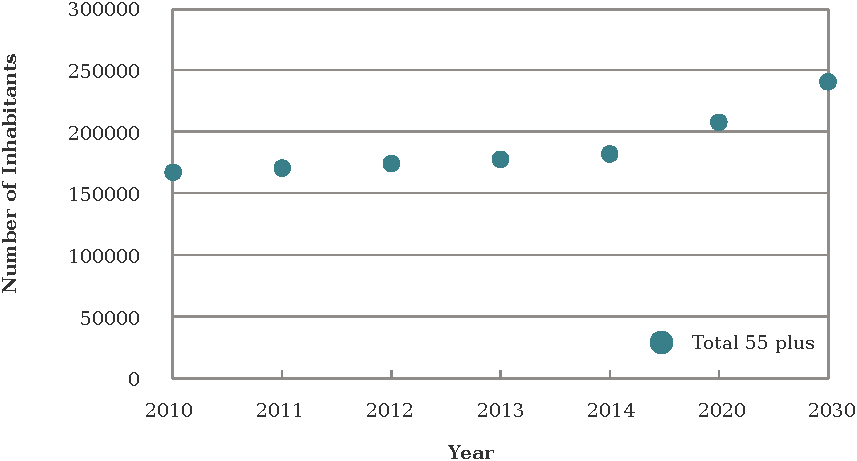
\includegraphics[width=\textwidth]{img/I1_number_elderly.pdf}
\centering
\caption[Total 55 plus inhabitants Amsterdam.]{
Total 55 plus inhabitants Amsterdam. On the 1st of January 2010-2014 \& Prognosis (2013) for 2020 and 2030. (Hylkema et al. 2014)} 
\label{demo}
\end{figure} 

Since 2015 the Dutch municipalities are responsible for the care of elderly, the assistance and support. The growing share of elderly is expected to demand higher funds regarding health care, social care and retirements wages but fewer funds are available for decentralized governments to spend on health care. These developments challenge to seek solutions to balance cost and services. Synergizing policy solutions between different policy areas at a decentralized level may help with the solution.~\cite{Hylkema2014} 

The new trend in elderly care is letting elderly live longer independently~\cite{MENSenSTRAAT2014, VandeRidder2008} also called active ageing~\cite{Annear2014}. The Amsterdam municipality aims its elderly strategy in the StructuurVisie for 2040 to let older inhabitants live independently, as long as possible, to reduce health care costs. Growing old in the own house, is welcomed by a lot of older inhabitants of Amsterdam.~\cite{Bossink2011}

\subsection{Elderly pedestrians}
Living independently means being mobile for personal care and have access to the public space for grocery shopping, social contacts and physical activity. In urban areas, elderly depend on walking for their everyday life and it is a key aspect of daily life to stay independent.~\cite{OECD2001}. Walking as form of transport happens more in urban areas then in rural(figure~\ref{walktrip}).
In many countries 30 to 50\% of older people's journeys outside are made as a pedestrian~\cite{Stahl2013}. In the Netherlands about 23\% of the trips made by elderly are made by foot. In Amsterdam 31\% of the main trips are made by foot. In general, Dutch elderly depend more on walking then other age groups as seen in figure \ref{percwalk} from a pedestrian study by CROW(explained in section 1.2.1).~\cite{Eijnde2011, Sauter2010, Crow2014}

\begin{figure}[h]
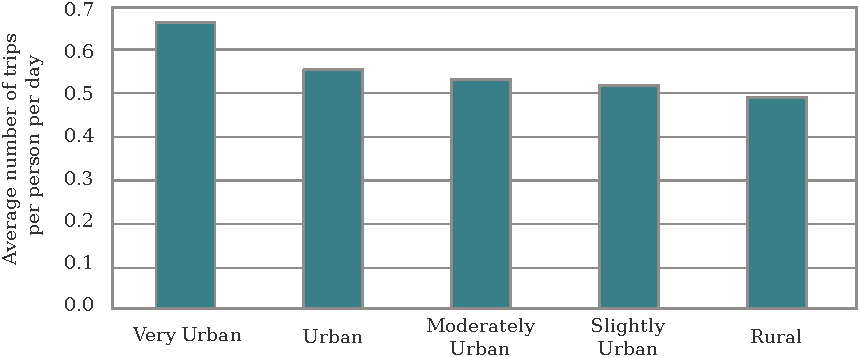
\includegraphics[width=\textwidth]{img/I2_urbanwalks.pdf}
\centering
\caption[Walking trips made in specific environment.]{Walking trips made in specific environment. (Sauter et al. 2010)
\label{walktrip}} 
\end{figure}

The main benefit of walking is the importance for the health of elderly.~\cite{Borst2008} Regular exercise has a positive effect on the fitness and physical health. Also lowering stress and improves the overall well-being. There is a well-established correlation between health benefits and regular physical activity.~\cite{Annear2014} Also, for elderly walking is the favoured form of physical activity.~\cite{Borst2008} See figure~\ref{percwalk}.

\begin{figure}[h]
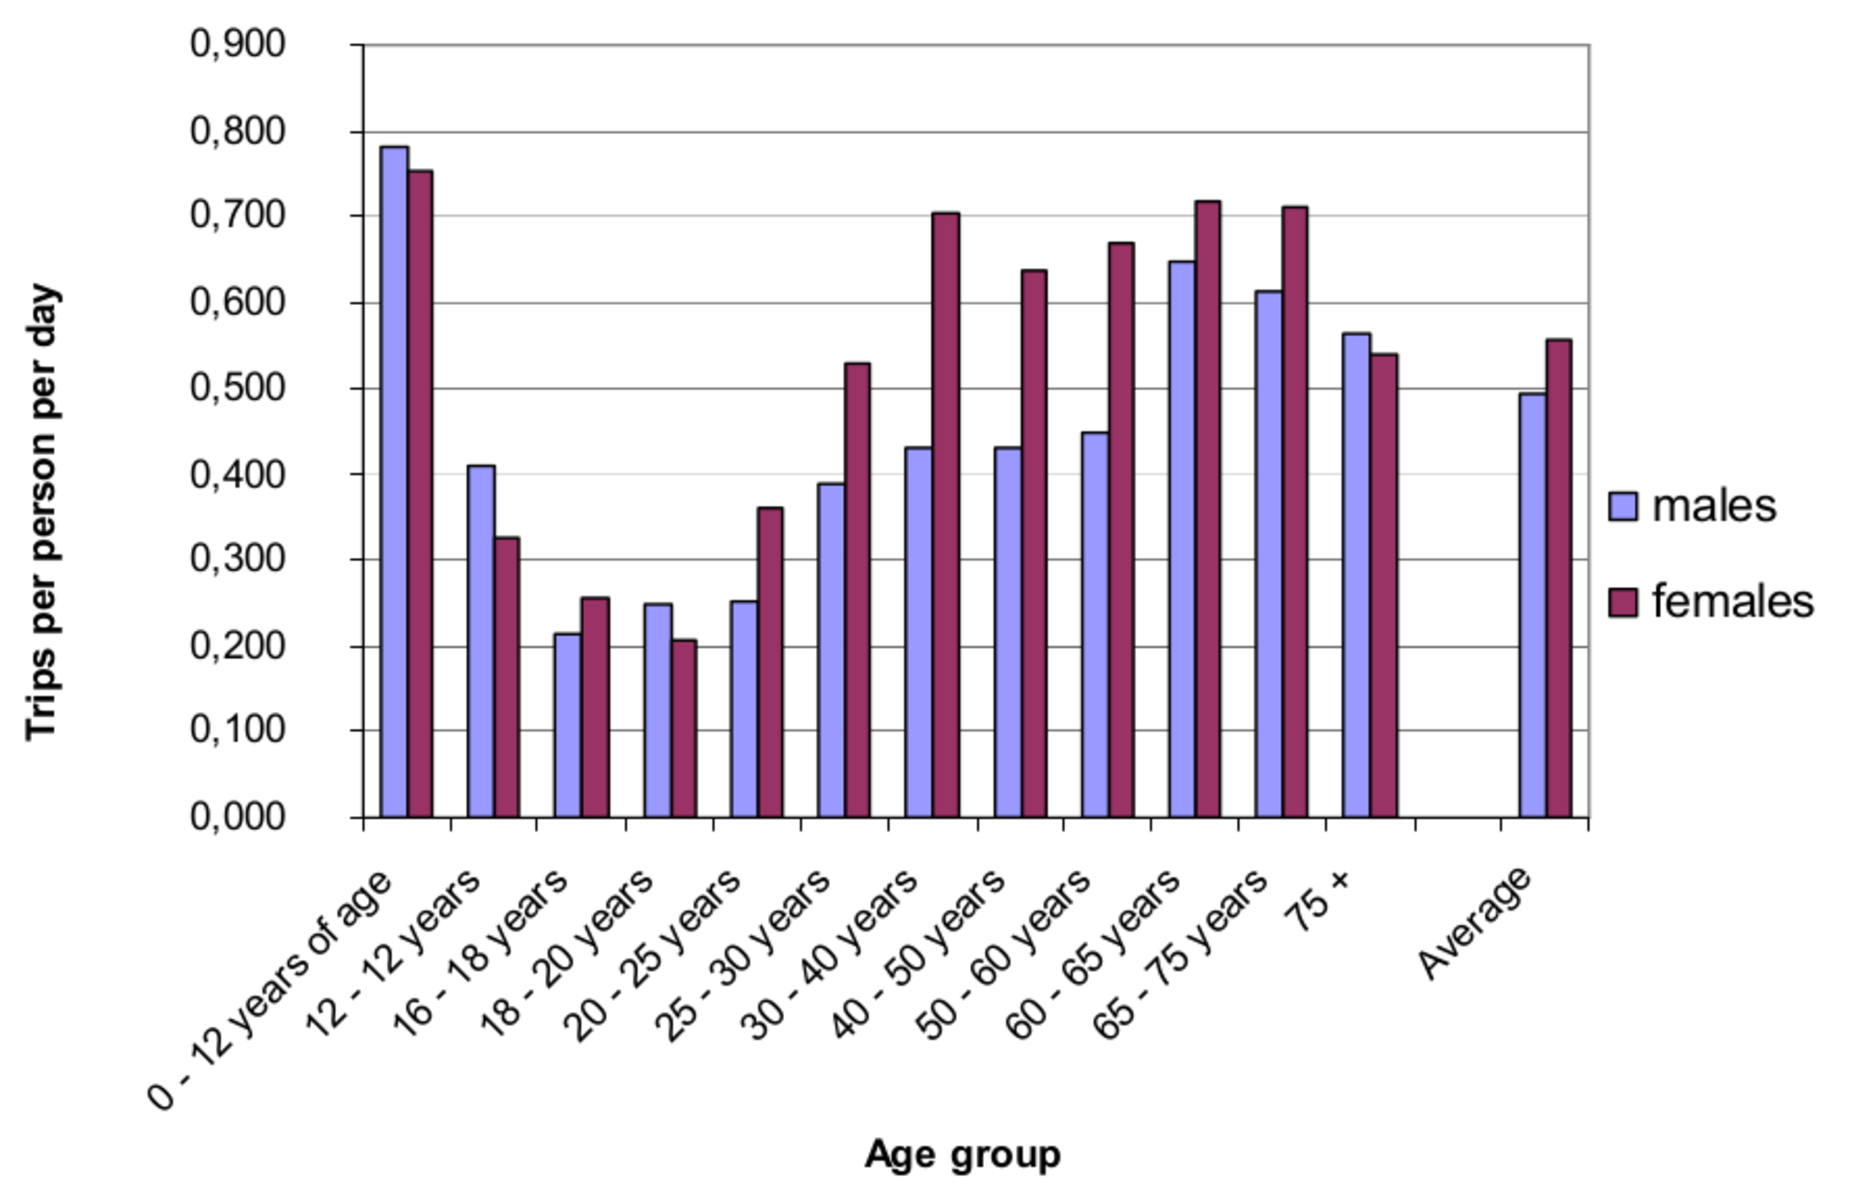
\includegraphics[width=\textwidth]{img/I3_numberOfTripsPerPersonPerDayByAge.pdf}
\centering
\caption[Number of trips per person per day by age group]{
Number of trips per person per day by age group. (NL, 2007 from~\cite{countryReport}) \label{percwalk}}
\end{figure}

In conclusion, outdoor physical activity, particular walking, seems the key role in the maintenance of functional independence at old age.~\cite{Rantakokko2009} By enabling mobility, elderly can keep control of their own life by being able to move outside independently for everyday tasks and social contacts.~\cite{MENSenSTRAAT2014} Walking keeps them fit and healthy and so increases the chance of longer and independent life. Overall, contributing to a better quality of life. 

\subsection{The Rollator}
A lot of elderly use a rollator, or wheeled walker. It helps maintaining mobility and continuing an active lifestyle. It provides stable support and may help avoid falls. Walkers are an important assistant for elderly who face difficulty walking and maintaining balance. The exact amount of rollator users in the Netherlands is unknown. An estimation in 2002 states 160.000 to 300.000 rollator users in the Netherlands~\cite{VeiligheidNL2012} with an average age of 77.7 years according to an article in Trouw.~\cite{Trouw2003} 
For further references we will refer to the wheeled walker as a rollator indicating a hand held walker with four wheels. 


\subsection{Mobility problems}
Getting older means; being less mobile and more fragile.~\cite{VeiligheidNL2012} In general, about 50\% of the pedestrians in the Netherlands have limited mobility abilities and around 10\% of the population has severe difficulties walking and sojourning in the public space.~\cite{Sauter2010} Table~\ref{nrpeople} shows the number of Dutch inhabitants with limited mobility, with the largest group formed by elderly above 65. Also the prediction for 2030 shows an increase in elderly with mobility problems.~\cite{Sauter2010} 

Yearly 18.000 elderly of above 55 need emergency care after a fall on the street. This means that every 30 minutes an elder adult falls so severe that care in the emergency room is needed.~\cite{VeiligheidNL2012} About 2.300 elderly of above 55, need emergency care after a fall with a rollator.~\cite{VeiligheidNL2012} One of the six falls with a rollator is outdoors. (380 falls a year)~\cite{VeiligheidNL2012}

Falls on the street without rollator occur more than falls with a rollator (18.000 to 2.300), but the latter cause more severe injuries. The medical costs for a fall with a rollator are inexplicably higher than a normal fall on the street(table~\ref{costsaccident}). An indication that a fall with a rollator leads to more serious injuries, then a fall with bike or scoot-mobile.~\cite{VeiligheidNL2012}

Fall accidents on the street occur due to behavioural factors (61\%) and environmental factors (58\%). Falls with a rollator can occur because a walker may be difficult to handle, the rollator is unstable or too heavy to handle for the user. A user needs strength and coordination to operate a rollator effectively~\cite{Einbinder2010, Weiss2014}. Environmental influences noted are irregular surface (43\%), obstacles and irregularities (31\%), bad maintenance (16\%) and slippery areas (13\%).~\cite{VeiligheidNL2012} One third of the falls on the street is because an elderly tripped (35\%) over a stone or tile (10\%) or a curb (4\%) and one fifth slipped (20\%) on a slippery surface (12\%).~\cite{VeiligheidNL2012} 

\renewcommand{\arraystretch}{1.5}
% \renewcommand{\tabcolsep}{6pt}

\begin{table}[h]
	\caption[Predicted number of people with limited mobility]{Predicted number of people with limited mobility, Netherlands (Sauter et al. 2010)}
	\label{nrpeople}
	\centering
	\begin{tabular}{|p{63.6pt}|p{44pt}|p{44pt}|p{44pt}|p{44pt}|p{44pt}|p{44pt}|} 
		\hline 
		-& 2005 & 2010 & 2015 & 2020 & 2025 & 2030 \\
		\hline
		Perc of people w limited mobility & 6.1 & 6.3 & 6.7 & 7.0 & 8.2 & 9.4 \\ 
		Number Younger than 65 & 340.000 & 340.000 & 350.000 & 350.000 & 360.000 & 360.000 \\
		Number 65 - 79 & 250.000 & 270.000 & 310.000 & 360.000 & 400.000 & 430.000 \\
		Number 80+ & 410.000 & 430.000 & 460.000 & 490.000 & 660.000 & 830.000 \\
		\hline
		Total number & 990.000 & 1.050.000 & 1.130.000 & 1.200.000 & 1.410.000 & 1.620.000\\
		\hline
	\end{tabular}
\end{table}

\renewcommand{\arraystretch}{1.5}
\renewcommand{\tabcolsep}{0.2cm}
\begin{table}[h]
\caption{Yearly average and total medical costs for 55+, to type of accident. From Letsel Informatie Systeem 2006-2010, VeiligheidNL~\cite{DenHertog2013} \label{costsaccident} }
\centering
\begin{tabular}{|p{236.2pt}|p{70.4pt}|p{70.4pt}|} 
\hline 
& Average costs & Total costs \\
\hline
Private- and traffic accidents on the street & \euro{} 4.500 & \euro{} 220m \\
Fall on the street & \euro{} 4.200 & \euro{} 82m \\
Simplex bicycle accident & \euro{}4.600 & \euro{} 71m \\ 
Rollator & \euro{}12.000 & \euro{} 33m\\ 
Scoot mobile & \euro{} 6.900 & \euro{} 8,9m \\
\hline
\end{tabular}
\end{table}

\subsection{The contribution of the built environment to walkability}
For elderly, who are more vulnerable, environmental attributes can be barriers to an active engagement in urban life. The quality of the immediate environment is a significant determinant of elders well-being, independence and quality of life.~\cite{Vine2012} Because these environmental details are critical for what the older inhabitants can manage in their everyday lives~\cite{Stahl2013, Stahl2008, Clarke2011, Annear2014} creating a walking-friendly environment is important for their independent mobility.~\cite{Sauter2010} The few studies that explore the older inhabitants and pedestrian-ism are arguing that good neighbourhood design can influence physical activity, health and consequently can lead to a longer life time of independence.~\cite{Vine2012, Rantakokko2009, Phillips2013, Beard2009, Rosso2011, Clarke2011}
The environment can have a powerful effect on the amount of walking activity undertaken by older people, thereby influencing their capacity to maintain their well-being and independence~\cite{Vine2012}.

The assessment of a neighbourhood design that supports elderly can be based on walkability. \begin{description}\item[Walkability] is the measure of how friendly the environment is to walking. The extent to which the built environment supports and encourages walking. By being friendly, giving comfort and safety, and provide aesthetic appeal.~\cite{Vine2012, Borst2008}\end{description}
% Vine et al. describes walkability as, the extent to which the built environment supports and encourages walking, by providing pedestrian comfort and safety, with reasonable time and effort and offering visual interest throughout the network. Borst et al. states that walkability is an index of the quality of the neighbourhood. The factors determining it, include, residential density, land-use-mix, street connectivity, aesthetics and safety.

A report from CROW, which is further explained in the next section, about pedestrianism in the Netherlands states that investing in pedestrian policy and making a pedestrian-friendly environment lets the elderly live longer independently.~\cite{Eijnde2011, Crow2014} This means, it requires the environment to provide the best conditions for even the most frail and weak sub-group.

Previous studies have found a relationship between neighbourhood characteristics, physical activity and related health aspects.~\cite{Borst2008} Aspects of the built environment, in particular neighbourhood design, have been found to influence the amount of physical activity undertaken by inhabitants of urban neighbourhoods,~\cite{Borst2008} access to public transport, nearby goods and services, walking for leisure, social interaction and engagement in the community.~\cite{Vine2012} In order to increase the quality of the environment, we need better insight into the influence of the urban design on the walking behaviour of elderly to make it useful for policy and design. 

\section{Problem definition}
\subsection{The forgotten pedestrian in policy}
There is little research carried out on pedestrian satisfaction in the Netherlands. The sparse information about what dissatisfies the pedestrian comes from complaints at local authorities, questionnaires or internet sites. The Pedestrian Quality Needs Project(PQN), identifies what people need for safe mobility in the public space. The project was conducted from November 2006 until November 2010. The main objective was to provide knowledge of pedestrians' quality needs to support walking conditions it the EU. They provide an extensive report on what people require as a pedestrian, and reports stating the current status of pedestrian knowledge in all participating countries.~\cite{Sauter2010} The PQN report of 2010 on walking in the Netherlands states that serious problems and deficits in Dutch pedestrianism are partly or totally hidden from public, scientific and political attention.~\cite{countryReport} They state the following about pedestrian knowledge in the Netherlands: 

\begin{description}
\item[The vicious circle] of no data- no awareness - no priority - no research - no data, needs to be broken.~\cite{Sauter2010, countryReport}
\end{description} 

With specific regard to elderly the PQN report states that large numbers of people already have trouble performing walking and sojourning tasks and because of the ageing of the population these numbers will only increase.~\cite{Sauter2010} Therefore, prevention of falls is important in regard to the safety of pedestrians which is also an age related problem.~\cite{Sauter2010}

The publication about pedestrians in the Netherlands from CROW (2014)~\cite{Crow2014}, states that pedestrians are forgotten in policy and design. CROW is a national knowledge platform for infrastructure, traffic, public transport and public space. A non-profit organisation providing guide-lines for the design, policy and projects with regard to the design of the public space. They state that walking, though one on the main forms of transportation, gets less attention then bicycles, public transport and cars. Pedestrians get more easily forgotten in policy design and maintenance plans. There is a need for a more systematic approach.~\cite{Crow2014} There are two reasons why walking is not part of policy and design plans; first, there is a lack of knowledge about how investments contribute to the tackle of problems. Second, there is no insight how walking can be optimised in policy, design and maintenance plans.~\cite{Crow2014}
With regard to elderly as pedestrians in specific, they state, that a well accessible pedestrian network, and attractive walking routes can contribute to the independence of elderly. Children and elderly are vulnerable in traffic, and elderly pedestrians above 75 have the biggest risk of being victim to traffic accidents with severe endings.~\cite{Crow2014}

MENSenSTRAAT is a network for independent mobility by foot or bike, focussing on the more vulnerable users of the public space. They constructed a pleading call for improving the public space with regard to elderly pedestrians and state that the direct outdoor environment, is crucial for elderly to live independent and stay healthy. Weak sub-groups are often overlooked in the design process and the local governments often forget the importance of street design for the elderly. MENSenSTRAAT states that this needs more attention.~\cite{MENSenSTRAAT2014} 

\subsection{The forgotten pedestrian in research}
Next to the forgotten pedestrian in policy, also little studies can be found on walking behaviour and pedestrians in general~\cite{Vine2012}. A limited number of studies can be found that look specifically at older people's use of the outdoor home environment, how they use it and what problems there are.~\cite{Phillips2013, Stahl2008} Even less studies focus on elderly walking with a rollator outdoors.~\cite{Stahl2008, Stahl2013, Phillips2013} Most studies about elderly, mobility and rollators focus on the interior conditions and accessibility indoors of public buildings, and residences.~\cite{Crow2014, Sauter2010, Verschuur2013} The outdoor environment is significantly important to elderly, but despite this, little research has been conducted on this topic.~\cite{Stahl2008} In addition, little knowledge exists about the factors influencing walking behaviour of elderly. What do elderly perceive as being unpleasant? Moreover, known factors do not always find an integrated place in policy, design and maintenance plans. Let alone, hardly any research can be found that focusses on methods to quantify or map possible problematic factors. 

\subsection{The forgotten pedestrian in data}
Because there is no research on pedestrians there is also no data~\cite{Sauter2010}. The PQN report gives several reasons for this lack of data:
\begin{enumerate}
\item Pedestrians are low on the transport agenda. Lack of sensitivity and political will on collecting data on walking. No counting means no data, no data means no counting.
\item Data that is collected is fragmented and inconsistent. There is a lack of common standards.
\item Indicators and methods for measuring transport are not appropriate for walking.
\item Existing information is not edited for use.
\item Existence of data is not known or hard to access.
\end{enumerate}

Another remark to make is that walking to other forms of transport, multi-modal walking, is almost as extensive as walking from door to door but is often not included in statistics.Therefore, the numbers are often underestimated in the interest of walking when looking at mobility statistics.~\cite{VeiligheidNL2012, Sauter2010} 

As long as the pedestrian is missing in the data, there can be no research and no actions taken to improve policy. While people that have mobility problems, are struck hardest by obstacles in the public space.~\cite{VandeRidder2008} 


\subsection{GIS opportunities}
% Mapping the urban area, to detect problems in order to solve them can be valuable for municipalities and urban planners to improve the situation for elderly and develop focussed interventions.~\cite{Stahl2013} 
% Because the physical aspects of the environment influence walking,~\cite{Leslie2005} 
GIS technologies and databases can provide great potential for studying the environment and neighbourhood characteristics that influences outdoor walkability quality among older people~\cite{Vine2012} and by doing so, fill a bit of the knowledge gap for decentralized governments and urban planners. While the role of geo-data in urban design is recognised nowadays,~\cite{Matthews2003} mapping the environment and the problems with GIS gives more understanding and customized information about the city to its city planners in order to develop new interventions and enhance walkability for rollator users.~\cite{Matthews2003, Svensson2010} GIS is a strong medium to provide urban planners with the data needed to make the urban area friendlier to rollator users and make cost-effective prioritized interventions. It is a rather easy approach to enhance the knowledge about the urban environment, and to locate certain obstacles and flaws that affect accessibility for the impaired citizens.~\cite{Svensson2010} Here we will look at the opportunities that available geo-data in the Netherlands and analysis provides to fill some of the knowledge gaps and make the obstacles for elderly pedestrians more visible. It helps to show that the build environment is often distorted and hostile for the mobile impaired.~\cite{Matthews2003}

\subsection{Lack of detail in (geo) data}
The scarce amount of studies about the elderly pedestrian, stated that more accurate, detailed and up to date data is needed to map walkability indicators for elderly, then the current and accessible geo-data can provide.~\cite{Verschuur2013, Laakso2011} Such detailed data is needed, because every stone counts in regard to frail elderly.~\cite{Matthews2003, Laakso2011} Importance of small details in relation to the larger infrastructure seems needed to map the walking restrictions in the outdoor activity space of elderly with a rollator~\cite{Stahl2008, Stahl2013}. Will GIS be able to map sufficient detail needed for the critical walkability indicators for elderly with a rollator? 

\section{Objective \& Research Questions}
The overall goal of this research is to create awareness of the forgotten pedestrian in policy, research and data. Awareness may trigger possible action at decentralized governments to increase walkability quality and so increase walking activity of elderly people. To keep them fit and healthy, capable to live independently and grow old in their own house and environment. All contributing to less need for healthcare for the growing share of elder population and reduce the cost of elder care.

The specific objective of this research is to analyse and visualize geodata to explore the critical walkability factors for elderly depended on a rollator in the urban outdoor space. The case study is set in Amsterdam, the Netherlands. To achieve this objective, the following research questions will be answered:

\begin{enumerate}
	\item What are the critical walkability factors hindering elderly with a rollator in the outdoor environment?
	\item Which existing geodata can be used to map and analyse these critical walkability factors?
 	\item What geodata can be collected with a smart walker to map and analyse these critical walkability factors? 
	\item How can the available and measured geodata be compared? 
\end{enumerate}

% This research aims at grasping the critical walkability factors that elderly experience while walking outdoors with a rollator and explore the possibilities of geo-data and GIS analysis to map and visualize them. This may increase walking activity of elderly people by raising more awareness and trigger possible action at decentralized governments. Consequently it can support health, the capability to live independently and grow old in their own house and environment. All contributes to less need for healthcare and so reducing costs for elder care. The case study is set in Amsterdam, the Netherlands. 

% The objective is, to analyse geodata of critical walkability factors for elderly people depended on a rollator in the urban outdoor space in favour of supporting outdoors walking activity. 

% % So the overall objective of this research is to analyse the critical walkability factors for elderly people depended on a rollator, in the urban outdoor space. T

% To achieve this objective, the following research questions are developed:

% \begin{enumerate}
% 	\item Investigate the critical factors for walkability in the urban outdoor environment for elderly depended on a rollator.
% 		\begin{enumerate}[a]
% 			\item Literature
% 			\item Experiences of rollator users
% 			\item Local government policy
% 		\end{enumerate}

% 	\item Map and analyse the critical factors by using available geo-data.

% 	\item Map and analyse the critical factors by collected geodata(measuring rollator movements with an accelerometer) and analysis.
	 
% 	\item Compare the available and measured geodata by anomalies in the time series data of speed, slope, and vertical acceleration, using changepoint detection.
% \end{enumerate}


\section{Report Structure}
This report exists of 5 chapters, including this introduction chapter. Figure \ref{reportstruct} illustrates the structure of this report. Chapter 2 describes some background concepts and projects related to this one, which are the inspiration and reference to support this study. Chapter 3 sketches the research area and continues to provide information, per research question, on data, preprocessing and methodology. The final chapter presents the conclusion, the discussion and gives recommendations for future work. Each chapter in this report opens with a short outline of its content.

\begin{figure}[hbp]
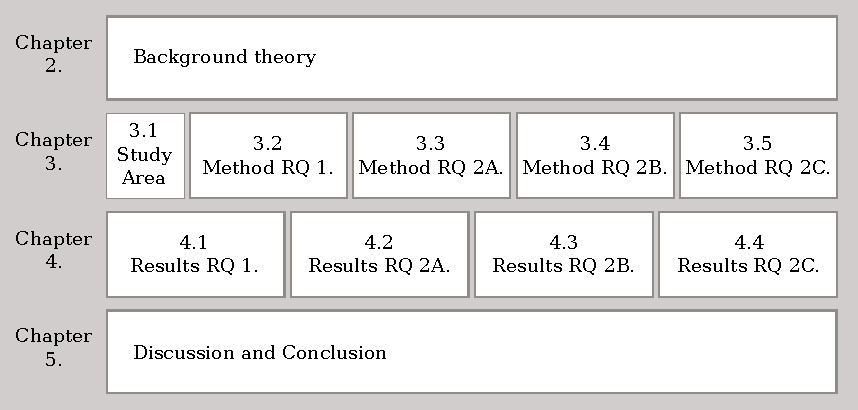
\includegraphics[width=\textwidth]{img/I4_ReportStructure.pdf}
\centering
\caption{Report Structure}\label{reportstruct}
\end{figure}
 
	\chapter[Background theory and concepts]{Background theory and concepts}
In sections \ref{pedestrians} and \ref{walking} some concepts used in this research will be clarified to have unambiguous use of terms. Section \ref{puccini} will tell more about the Puccini method which is used for the design of the public space in Amsterdam. 
This chapter will be finished with summaries of related literature (section \ref{literature}) which helped forming this research and provide reference and support for the data and methods used.

\section[Pedestrians]{Pedestrians}\label{pedestrians}
\begin{description}\item[A pedestrian] is a person, by foot, with or without helping aids, that moves in the public space. The person is not a driver but a road user. Also persons with a wheelchair, rollator, roller-blades, skateboard or children's bicycle, as well as persons walking with a bike, scooter or motorbike in the hand are pedestrian according to the Wegenverkeerswet voetganger.~\cite{Crow2014}
\item[Mobility] is the freedom to choose to travel and sojourn in the public space, being able to make the trip, regardless its distance. Pedestrian mobility differs from other modes of transport, for it almost part of all other trips.~\cite{Sauter2010}
\item[Sojourning] is an important indicator for quality of public space, it includes activities as; recreational walking, waiting and hanging out in the public space.~\cite{Sauter2010} \end{description}

The Netherlands is climatic and geomorphological very favourable for walking.~\cite{Sauter2010} In cities almost all streets have two sided side-walks.~\cite{Sauter2010} Though, cycling is perceived much more important in the Netherlands as seen in the pecking order in traffic: public transport, car traffic, scooter, bicycle, pedestrian. In some regions of the Netherlands the soil is rather soft and peaty, in these circumstances the pavement has to be renewed every few years, to prevent sinking.

\subsection{Walking behaviour}\label{walking}
The rate of walking for a person is determined by many factors, environmental influences, personal influences or behaviour and biological influences. Here we focus on the environmental influences, in specific, walkability of the environment. Walkability is one of the many important determinants that influence the walking behaviour of elderly~\cite{Vine2012}. Here we try to sketch an overall overview of these determinants, according to the behaviour scheme of Bartolomew, ~\cite{Bartholmew2011} to show where walkability is positioned, next to terms like accessibility and mobility. 

The scheme in figure~\ref{behaviour} represents a small part of the personal and environmental determinants that influence the criteria for walking behaviour of elderly. It is incomplete as this is not a behaviour study, but gives a good insight in what is and is not included into the term walkability. 
First of all, the personal determinants like personal health, previous experiences and perceived self/efficiency are not part of this study. Though, what not to forget is, that these can be greatly influenced by the environmental characteristics. 

Walkability is part of the environmental determinants, terms used in dedicated studies are accessibility, walkability, safety and activity space.~\cite{Vine2012} Accessibility is the ability to access needed facilities and enable persons with disabilities to gain access through for example elevators, audio signals, walkway contours etc.
As stated in the previous section, mobility is the freedom to travel in the public space. Here we assume that all elderly have the freedom to go outside, make use of the public space and access the facilities they need.

The quality of these routes, the friendliness and the safety are gathered in the walkability determinant. So while a person in walking and accessing the public space, how user friendly and how much effort does it cost to cover these routes?

\begin{figure}[h]
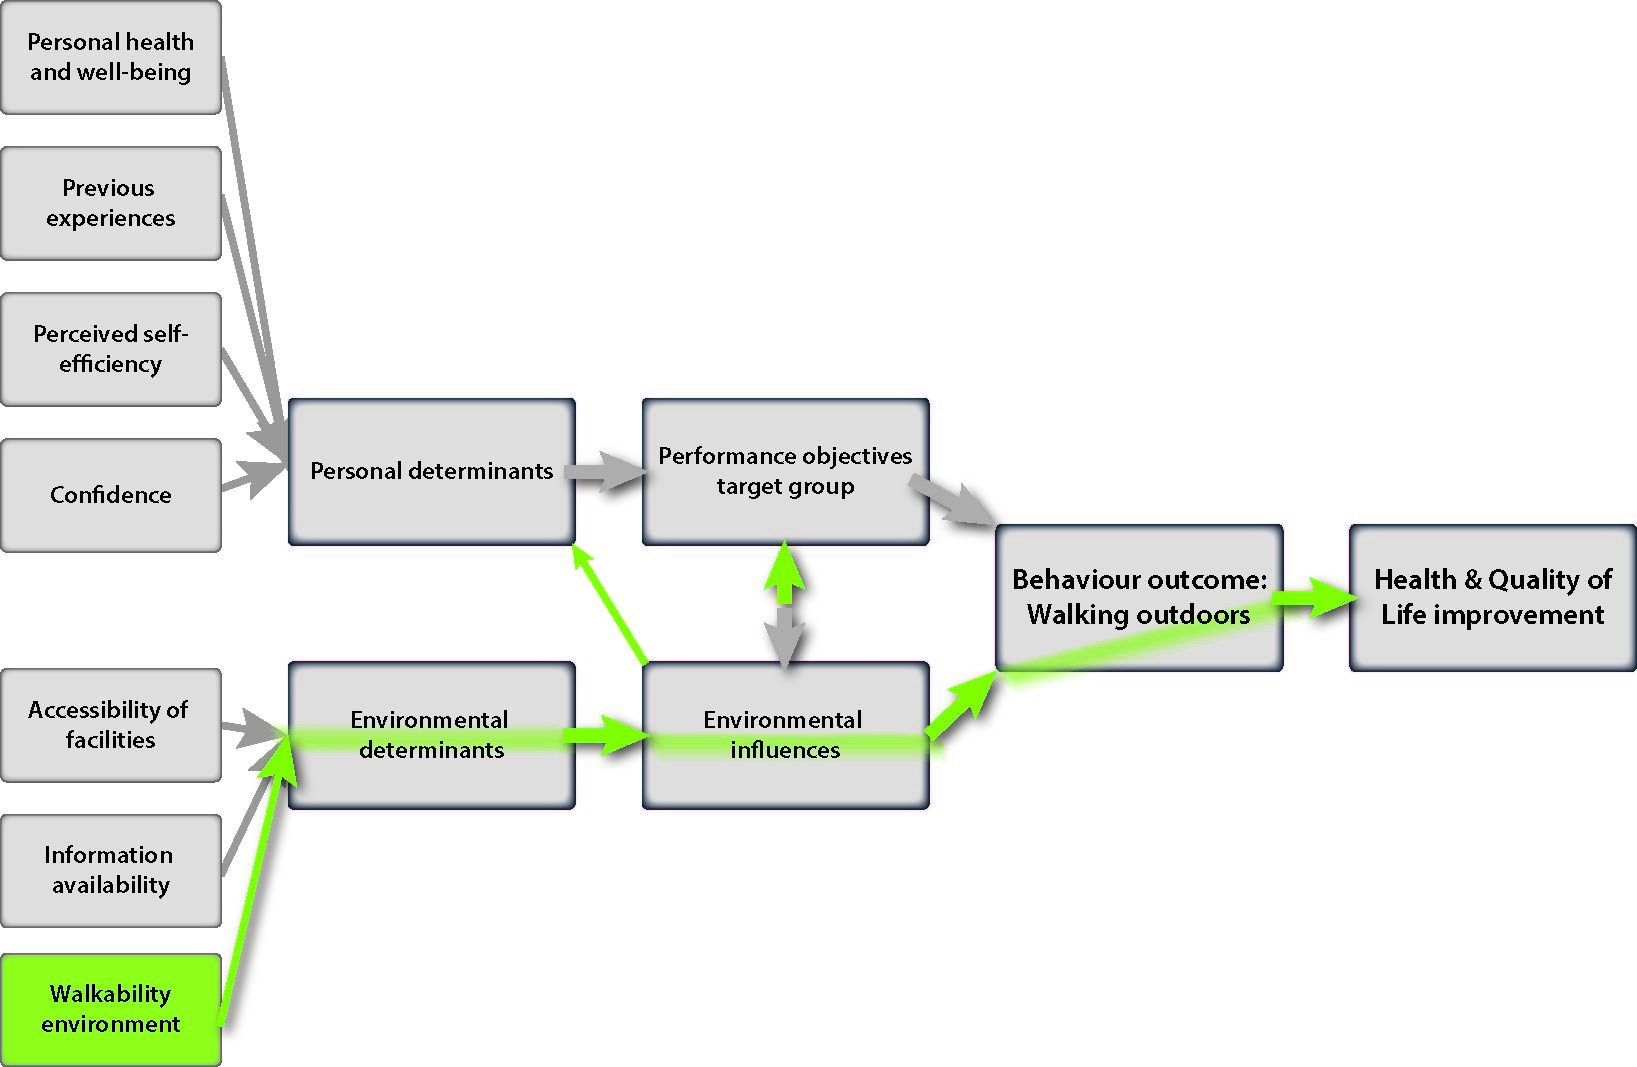
\includegraphics[width=\textwidth]{img/B_Behaviour_Scheme.jpg}
\centering
\caption[Walking Behaviour Scheme]{Walking Behaviour Scheme (Source: Boeijen, based on Bartholomew 2011)
\label{behaviour}}
\end{figure}

The individual path selection criteria of Golledge can be placed next to  this scheme to show how they influence the actual choice for walking. All the personal and environmental determinants together, make an individual decide to go by foot or not to a certain destination. Then when choosing the route and having experiences on these routes influence the choice for the next time the user wants to walk that route and which path will be followed.~\cite{Golledge2002} The individual path selection criteria by Golledge knows 3 phases: 

\begin{enumerate}
\item Choosing destinations 
\item Making a route 
\item Implementing and feedback. Confirmation or change?
\end{enumerate}  ~\cite{Golledge2002}

The first two phases are influenced by the many determinants, while the last phase provides new knowledge and experience again influencing the next time a user wants to walk outside. Increasing or decreasing the influence of the previous determinants. 


\section{Walkability factors}
From several literature studies dedicated to pedestrian-ism, elderly pedestrians, mobile impaired pedestrians, rollator users, walkability studies and walking behaviour, a list of possible walkability criteria for elderly with a rollator is created. The criteria are influenced by a wide variety of factors of the urban environment. They can be tangible and physical or intangible and more related to personal perception and feelings. ~\cite{Verschuur2014} Some criteria focused more on the broad environment of living, while others more on personal detail in the direct environment. 
Already, several other studies made an overview of walkability criteria for elderly or the mobile impaired. For example ~\cite{Verschuur2014} provides a list of parameters affecting route attractiveness and the studies in which its found. Also ~\cite{Duncan2011} provides a whole list of walkability indicators they use for calculating a walk score. Rosenberg ~\cite{Rosenberg2013} provides a summary of barriers and facilitators in the built environment. Wennberg studies a whole list of usability factors and their statistical significance, divided into categories, physical barriers, orientation and warnings, bus stops and shops, orderliness and benches and stairs. ~\cite{Wennberg2009} All these lists and other studies are used to create an own overview in order to filter out the most important walkability criteria for elderly with a rollator. This list can be found in Annex \ref{Acriteria}

For making all the criteria more orderly, they are first subdivided into tree levels of where they could occur. 

\begin{enumerate}
\item Pavement level
\item Street level
\item Environmental level
\end{enumerate}
Though, this didn't seem sufficient, some weather related and temporal issues that occur, could not be placed in this subdivision as they can occur over all these tree levels. Also crossings form a own special nice in the levels for it is not part of the pavement or the street. Therefore these are added to the tree levels mentioned above.
\begin{enumerate}
\item Weather or temporal level
\item Crossings
\end{enumerate}

Also the factors could be assigned to different categories, some had to do with accessibility and other with the quality of the environment. Five categories can be distinguished. These are inspired by ~\cite{Ballester} and ~\cite{Rosenberg2013}.

\begin{enumerate}

\item Accessibility
\item Quality 
\item Obstructions or barriers
\item Route attractiveness 
\item The feeling of safety
\end{enumerate}

Accessibility is about the access and presence of the pavements, if there is a pavement available and destinations can be reached. Some examples of factors are: the availability of public transport nodes,  availability of bridges, availability of ramps to the pavement a.o. 
The quality is about when a pavement or stair is present, what the quality is. This could include things as a non slippery pavements, the slope of bridges and the slope of the pavement. 
Obstruction contains tangible objects that are in the way, temporary or stationary.  Like protruding portals and facades, blocking commercial signs or green maintenances so branches are not hanging over the pavement.
Route attractiveness is more about the feeling one has towards the routes, the attractiveness can go down with the presence of dog droppings on the pavement, litter and garbage on the streets. While it can go up with the availability of resting benches, public toilets, green and trees along the route. 
The feeling of safety includes factors as enough time to cross the street, good overview while crossing a street, vehicle-pedestrian interaction, speed limits, presence of street lights, the amount of criminality and many others. 


\section{Puccini Method}\label{puccini}
The Puccini Method is the Amsterdam tradition for the design of the public space and formulates design principles. Public space includes all non-build-up space, open and accessible to people. The Puccini Method contains all points of policy, to the detailed design, technical details and material lists. It contains four modules, red for streets, green for vegetation, blue for water and water banks, and last, purple for street furniture, street lights and public transport stops. 
The Puccini method is the handbook for the municipality to maintain and design the public space. It is not a policy design book.~\cite{puccini2014}

The Puccini method contains 6 convictions:~\cite{puccini2014}
\begin{enumerate}
\item 	\begin{description}
		\item[Choose, not share] 
		The streets are used more intensive and pressure increases. Often the usage pressure is higher then the available physical area. Therefore the available space has to be assigned to one use, not shared. 
		\end{description}
\item \begin{description}
		\item[Simplicity and obviousness] 
		The pbulic space should be user-friendly, sustainable, strong in simplicity, timeless and obvious. With simple material and simple design, reaching for good quality.
		\end{description}
\item \begin{description}
		\item[Craft and skill as a basis] Craft expertise is the basis. Not only designing inside, but going out on the streets with work experience is the key. 
		\end{description}
\item \begin{description}
		\item[Crucial eye for detail] Detail for material use, time, financial resources and facing problems that have to be solved. 
		\end{description}
\item \begin{description}
		\item[A good plan is maintainable] After the realization of a street or square it still has to be maintained. The plan has to take the maintenance into account for the future. 
		\end{description}
\item \begin{description}
		\item[Cooperation] A lot of specialised disciplines are concerned. Throughout the whole process it is important to communicate until the end product is realized. 
		\end{description}
\end{enumerate}

Amsterdam is a cultural historic city, with many urban designs from different time periods. The historical city centre, the 19th century canal-belt, the 20-40ties en the postwar city.  The urban design has to suit the cultural historic character of the city. For every urban style zones there are material lists and standard design details.~\cite{puccini2014} A map of Amsterdam indicating where each urban time zone is located can be found in annex \ref{pucciniMap}.
	
\section{Related literature}\label{literature}
Form the few studies that do focus on elderly pedestrians some perceived as helpful for this study will be discussed in this section.
The most important researcher aiming at the elderly as a pedestrian outdoors is Agnete St\"al. The rollator is a Swedish invention, and St\"al is a Swedish researcher focussing a lot on elderly pedestrians with rollators, about their accessibility and safety in the public space and how interventions in the public space impact the elderly pedestrian.   

Literature that discusses the possible methodologies to make walkability quantifiable are often found under the term Smart Walker. The studies from Wang and Weiss  et al. focus more on the technical aspect of measuring rollator movements. 

The only study combining the pedestrians perception with measuring the helping aid is a study by Matthews at al. Though, here it is more focussed on wheelchair users, it can easily be translated to rollator users. 

\subsection{Critical walking factors for elderly with a Rollator}
Stahl is one of the few that looks at the elders perception of the built environment and how specific interventions can help rollator walks be perceived more attractive.~\cite{Stahl2008, Stahl2013}

The measurements most mentioned are:
\begin{enumerate}
\item Separation of pedestrians/cyclists
\item Lower speed limits
\item Better maintenance
\item Wider side walks
\item Decrease curb levels
\item More even surfaces on pavements
\end{enumerate}~\cite{Stahl2008}


\subsection{The Smart Walker}

There are a few researches on making a rollator more smart by using sensors; the Smart Walker. Most of these studies focus on fall protection, early warning systems or indoor navigation. There are functions such as sensor assistance, health monitoring, navigation help or cognitive assistance, obstacle avoidance and fall detection.~\cite{Wang2015} 

Most studies using an accelerometer as a sensor, calculate gait parameters such as; step length, gait cycle, step width and gait variability.~\cite{Wang2015} 

Often these studies are done in laboratory settings, using high quality sensors and sensors attached to the body.
This research aims at obstacle detection, with the help from detecting the movement of the rollator. On this, no specific literature could be found.

\subsection{Using an accelerometer for rollator monitoring}

Weiss et al. (2014) uses a smart walker to detect walking behaviour change in real time with an accelerometer mounted on the rollator.~\cite{Weiss2014} No sensor on the user is needed, but the walking behaviour is detected based on the motion transfer by the user on the walker. The goal is to identify five different classes: no movement, movement, slow, normal and fast. They confirm that walking behaviour changes can be detected by using a 3-axis accelerometer sensor on the walker.


\begin{figure}[h]
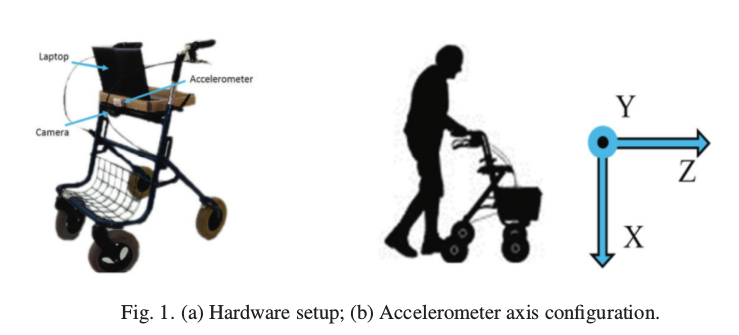
\includegraphics[width=0.75\textwidth]{img/B_Weiss.png}
\centering
\caption[Rollator with accelerometer axis configuration]{Rollator with accelerometer axis configuration. From Weiss et al.~\cite{Weiss2014} \label{rolaxis}}
\end{figure}

Wang et al. (2015) uses a standard 4-wheel rollator with a defined walking frame, where the accelerometer is positioned in the middle point between the two rear wheels. By doing this the exact distances to the wheels are know and from this the position change of the walker can be determined. By using a high cost motion capture system, the calculated trajectory's and the gait or step detection, are validated. Wang was able to calculate the displacement of the walker during every step with an accuracy of approx 1 cm.~\cite{Wang2015} By comparing a group of young adults with group of elderly people, Wang found the the walking accuracy of the elderly is lower but that step length, step period and walking speed between the two groups has no obvious difference. The classical gait indicators are not sufficient or sensitive enough to evaluate the fall risk of elderly.~\cite{Wang2015}
 
\begin{figure}[h]
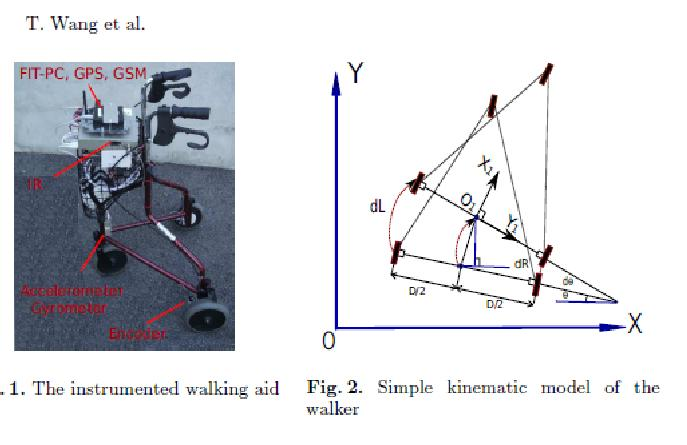
\includegraphics[width=0.5\textwidth]{img/B_Wang.jpg}
\centering
\caption[Rollator set-up]{Rollator research set-up. From Wang et al.~\cite{Wang2015} \label{rolsetup}}
\end{figure}


Both Wang and Weiss made use of a non-intrusive measurement method. Were no devices were placed on the participants but only on the rollator. 


\subsection{Outdoor quality for Wheelchair users}
Obviously, a wheeled walker and wheelchairs have a lot in common. Therefore, also literature studies aimed specific at wheelchairs can provide useful insights for rollator research. 

Matthews et al. 2003 uses a GIS based system to show that the built environment is often distorted and forms a hostile space for wheelchair users.~\cite{Matthews2003}

Small test were conducted measuring surface hindrance for wheelchair users, aiming at surface type and quality for mobility. Six common urban surfaces were tested: concrete, paving, tarmac, brick, grass and gravel. A wheelchair with occupant was pushed down a small ramp the distance rolled provides an measure for rolling resistance. 

\subsection{Elderly perception of the outdoor environment}
Ideas from Hogertz, 2010 ~\cite{hogertz2010} 
	\chapter[Data and Methods]{Data and Methods}

This chapter starts with a small section on the research area. \ref{area}
Then, per research question a section is dedicated, describing its data, pre-preprocessing steps and the analysis. The critical walkability factors will be explored in section \ref{rq1} through literature studies and interviews. Also a short sub-section on the average walking speed of elderly is present. 
Section \ref{rq2a} shows the data collection and pre-processing steps for the analysis of existing geo-data. The GBKA an the AHN are used.

In section \ref{rq2b} the data collection and pre-processing steps for the collection of our own geo data, with GPS devices and an accelerometer. Eventually, the steps for analysing this data is explained in the last part of this section.

The methods for combining the existing geo-data with the own collected data is explained in section \ref{rq2c}. With a Change Point detection algorithm, changes in the time series of the rollator walks are found, and plotted on the map to compare it to other data sources. 

\section{Study area}\label{area}
This project in conducted for the project MeetRollator in the scope of the recently founded Amsterdam Institute For Advanced Metropolitan Solutions (AMS). The study area of AMS in Amsterdam, see left figure ~\ref{kaart} for the location. The Amsterdam Municipality contributed with data that covers the centre area of Amsterdam, indicated with the red square in the right figure ~\ref{kaart}. 

The literature study, interviews, AHN study will be mostly focussed on this area. The more general measurements were taken in Wageningen due to a more conventional location and travelling circumstances for the conducting researcher. See figure ~\ref{tracks} from chapter 3.5. 

There is no exact information on the amount of elderly using a rollator in Amsterdam or where they live. There for the CBS statistics of 2013 were used to detect the neighbourhoods were the most elderly above 70 live. In figure ~\ref{kaart} can be seen that in the centre the most elderly live in the Jordaan. In the whole of Amsterdam the most elderly can be found in the South West and North.  

\begin{figure}[ht]
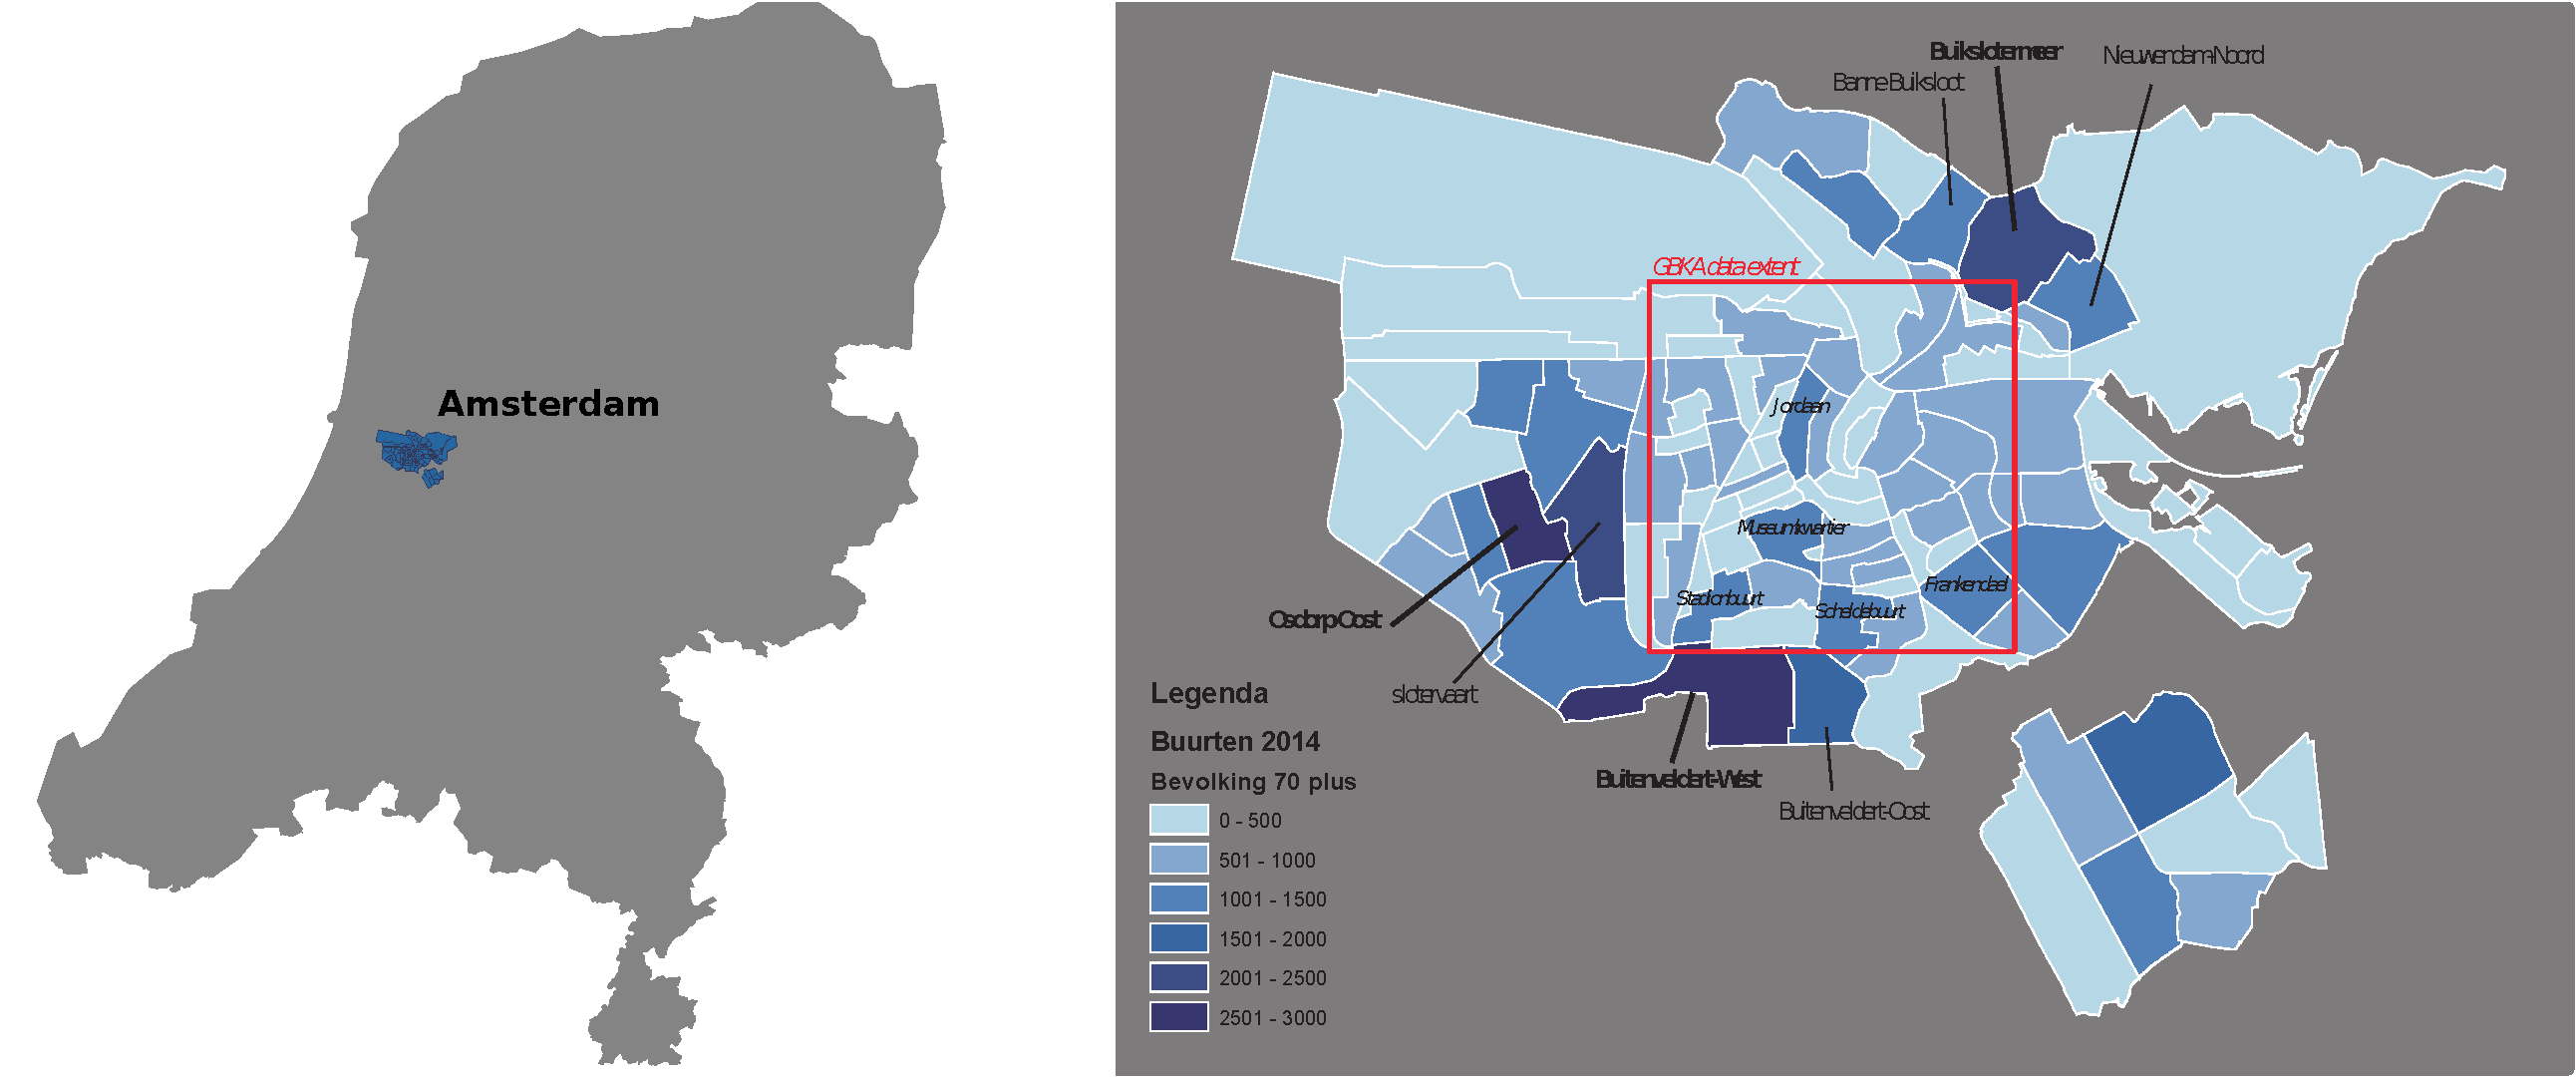
\includegraphics[width=\textwidth]{img/SA_StudyArea.pdf}
\centering
\caption{Study area Amsterdam, The Netherlands\label{kaart}}
\end{figure} 
	\section{Method RQ 1 - Finding the critical factors for walkability}
\subsection{Literature study}
From literature research, all possible problems that elderly with a rollator can encounter were gathered. Together with the extend of the problem importance. This to form the first main idea of what the possible critical factors could consist of and the eventual list of findings will be used to support and design the interviews with the elderly and finding requirements in the policy and design policies.
The literature study was conducted from October 2014 until January 2015. 

\subsection{Interviews}
In the initial idea was an interview that would consist of 3 parts; first a general part, about age, health and the use of the rollator. The second part is a list of possible problems the participant could encounter. The third part would be drawing on a map, where the participant walks and where certain problems occurred. See overview ~\ref{interview}. Though after developing and experimenting the final form and the method of conducting changed quickly. 

\begin{figure}[h]
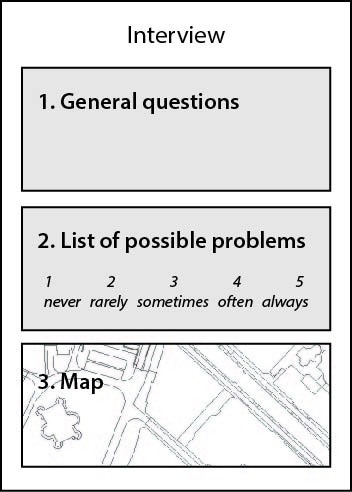
\includegraphics[width=0.25\textwidth]{img/M_interview-01.jpg}
\centering
\caption{The 3 parts of the interview \label{interview}}
\end{figure}

The questionnaire as shown in Annex \ref{Aquest}, consisting of several pages was developed. The questionnaire was tested, with the researchers grandparents. This concluded that the questionnaire is not a good form for obtaining information form elderly. The reaction of the participants was, that things were unclear and not all questions were answered.  Also the amount of text scared the elderly, feeling uncomfortable with their abilities of reading and writing. Therefore, the form of the interview quickly changed to an informal chat, were the researcher used a check-list, making sure all questions were asked while chatting in random order.
\newline
The second part, containing a list of possible problems the elderly could encounter was constructed after the literature research. 5 categories are constructed:

\begin{itemize}
\item Quality of the pavement
\item Obstacles
\item Overall business
\item Safety feeling
\item Environmental characteristics
\end{itemize}

The total list can be found in annex~\ref{Aelderly}. For the elderly did not feel like reading too much, also this part of the questionnaire was conducted oral. Every possible problem on the list, were read out loud to the elderly and asked to rate from 1 to 5, 1 is they never encounter the problem to 5; they always encounter the problem. The conducting researcher circled the number from 1 till 5 according to the story of the participant. 

The third part, drawing or pointing out problems on a map was quickly cancelled, as the elderly had difficulties reading the maps. They did, though, name streets and locations but the conducting researcher was too unfamiliar with the surroundings to translate this quickly onto the map. 

Several elderly care houses were contacted as well as the neighbourhood care of Amsterdam centre. While sounding enthusiastic from the first point, it was hard to arrange appointments with elderly. 

The total amount of participants for personal interviews were only 2. 

Next to this, also participants on the Rollator Loop were interviewed. Around 10 people were shortly interviewed about the general problems they encounter while walking outdoors. But not the complete list. 

\subsection{Rollator Loop - Average walking speed}
We visited the yearly event, the Rollator loop in Amsterdam on the $9^th$ of September 2015. Here we conducted interviews, measured several walks and gained overall information about the walking performances of that day. 

Little information can be found on the internet about the general walking speed of elderly with a rollator. Because the opportunity was there to find out more about the average walking speed of elderly with a rollator, this was conducted as well. MySports, a company for time tracking during sport events, measured the walking time of every participant.~\cite{mysports} The outcome of the Rollatorloop 2015 and 2014 were used to do a small side study on walking speed per distance and gender. 
	\section{Method RQ 2 - Collection and analysis of available geodata}\label{rq2a}
Data was available on walking speed, topology of Amsterdam and a height map of the Netherlands. The average walking speed was conducted as input for choices in research question 3 and 4. The topology provided a basic map of the available pedestrian area and the height map gave insight in sloping pavements. 

\subsection{Rollator Loop - Average walking speed}
We visited the yearly event, the Rollator loop in Amsterdam on the $9^th$ of September 2015. Here we conducted interviews, measured several walks and gained overall information about the walking performances of that day. 

Little information can be found on the internet about the general walking speed of elderly with a rollator. Because the opportunity was there to find out more about the average walking speed of elderly with a rollator, this was conducted as well. MySports, a company for time tracking during sport events, measured the walking time of every participant.~\cite{mysports} The outcome of the Rollatorloop 2015 and 2014 were used to do a small side study on walking speed per distance and gender. 

\subsection{Data Collection and Pre-processing - Topology }
The municipality of Amsterdam, provided the GBKA (grootschalige basis kaart Amsterdam). The GBKA is the precursor of the BGT (basisregistratie grootschalige topografie) which will be used after 1 Jan 2016: the basic registration of large scale topography. The GBKA is obtained, maintained and provided by the municipality. It contains information about transport, water, buildings, street furniture, land use and public space.~\cite{gbka} The GBKA is delivered in file format ESRI Shape files and is projected in RDnew. 

Next to this also the website amsterdamopendata.nl is consulted for extra data.~\cite{opendata} The data downloaded form amsterdamopendata are CSV files containing the $X$ and $Y$ coordinates in RDnew and WGS84. The CSV files are opened with Qgis and transformed to Shape file to work with the rest of the data. 

\subsection{Analysis - Determining pedestrian area with GBKA}

The detailed GIS study will be done on the area Jordaan in Amsterdam. The Jordaan is part of the Historic Centre belt form the Puccini method. (Gordel Historische kernen) This means most pedestrian pavements and streets are made out of baked red bricks. \cite{puccini2014}
The GBKA contains polygon features for road sections. Though, these do not contain a label, indicating which purpose of use it has. See \cite{gbka}. The first step will be to see if it is possible to derive the pedestrian area from available data. The Puccini method contains 6 classes for road destination \cite{puccini2014}, see the list below. Though this distinction is not used in the geo data available at the municipality.

\begin{enumerate}
\item Pedestrian
\item Bicycle
\item Public transport
\item Trees and street furniture
\item Cars (moving)
\item Cars (Parked)
\end{enumerate}

For analysis, this research we are only interested in the pedestrian area, so the distinction between areas to walk on safely, and areas not walked on safely is made. The classes from Puccini are simplified to 3 classes, were mixed space is not taken into consideration.:
\begin{enumerate}
\item Transport: Cars, bikes, public transport. 
\item Pedestrian area : Including square, stairs, parking places. 
\item Unpaved: trees, parks, bank, garden.
\end{enumerate}

First, all the road sections of all levels are merged with the bridge features and clipped to the Jordaan neighbourhood. A new column is created, class, to assign 1,2 or 3 to according to the purpose of use. 
Figure \ref{classRoad} shows the decision tree of steps taken to assign the three classes to the road sections. The classification process starts from the top to the bottom, in every step assigning the selected group the class and continuing with the features which do not have a class assigned yet. The first steps are done by selecting criteria on the available attributes of the road sections. After this other shape-files from the GBKA are used to derive pedestrian area and the tool selection by location is used. For example, street furniture is often placed on the pedestrian area and not on roads for moving cars. In the end, all remaining sections are assigned class 1 transport. All data is from the GBKA except the parking lots which are downloaded from www.amsterdamopendata.nl. 

\begin{figure}[ht]
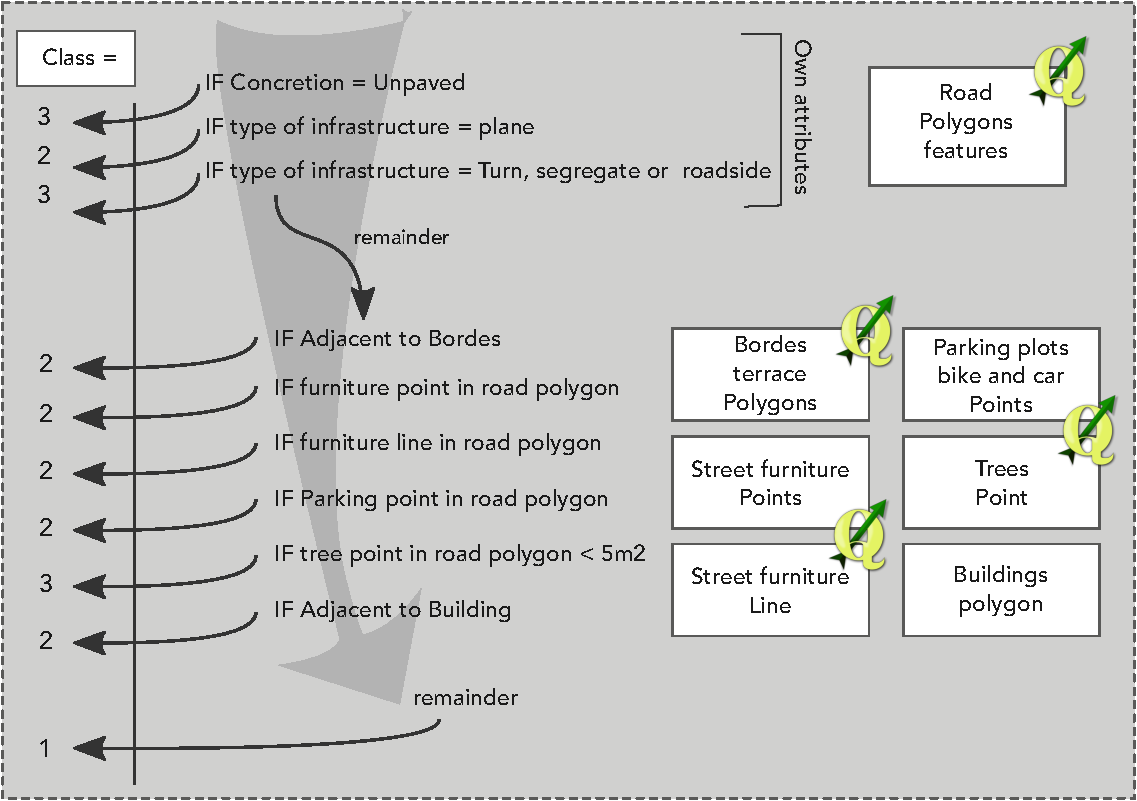
\includegraphics[width=\textwidth]{img/M_Pedestrianareaclassification.pdf}
\centering
\caption{ Classification steps road sections\label{classRoad}}
\end{figure}


\subsection{Data Collection and Pre-processing - AHN }
The AHN2 tiles covering the research area were downloaded from www.nationaalgeoregister.nl. The AHN is measured with laser altimetry or LIDAR. Laser beams shot from an air plane and localized with GPS. It is measured over several time periods and merged in the end to get a detailed measurement of the height. With a measured point density of 6 to 10 point per $m^2$~\cite{VanDerZon2013}. The eventual end product delivered is corrected to ground level, so vegetation, buildings and other object do not appear.~\cite{VanDerZon2013} These filtered areas are given no-data values. The raster data has a resolution of $0.5m^2$ and a precision of systematic and stochastic error of max $5cm$. The projection is the Dutch projected coordinate system RD new.~\cite{VanDerZon2013} Because the AHN2 is already delivered in RD new and corrected for ground level, no or little pre-processing is needed. Apart from downloading the correct tiles and merging these together for the appropriate area. 

\subsection{Analysis - Mapping sloping surfaces with AHN data}
The Policy of Amsterdam states that pedestrian areas with slopes more than 4\% is perceived negative.~\cite{leidraad2011}
The slope is derived from the AHN2. Also per road section, the average slope is calculated. The pedestrian classification with the GBKA are used to compare road sections for transport versus pedestrian area. 

\subsubsection{First derivative - Slope}
The first derivative or slope provides the degree of slope per pixel. This can be calculated with the following formula on cell to cell basis. 

\textbf{Degree of slope:}
\begin{equation}
\tan \theta = \frac{rise}{run}
\end{equation}
~\cite{ahnformula}

\textbf{So slope in degrees:}
\begin{equation}
\theta = \tanh \frac{\sqrt{\frac{dz}{dx}^2 + \frac{dz}{dy}^2 }*180 }{\pi}
\end{equation}
Source: ESRI 
http://webhelp.esri.com/arcgisdesktop/9.2/index.cfm?TopicName=How\%20Slope\%20works~\cite{ahnformula}


% \subsubsection{Second derivative - Curvature}
% Curvature is the second derivative of the surface, or the slope of the slope. Positive curvature is upward convex and negatives curvature is upward concave, at the cell. A value of 0 is a flat cell. The curvature of a surface is calculated on a cell-by-cell basis. For each cell, a fourth-order polynomial is calculated of the form:

% \begin{figure}[ht]
% 	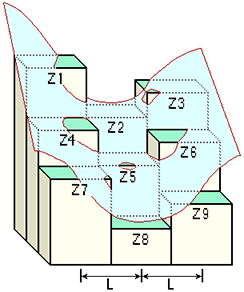
\includegraphics[width=0.25\textwidth]{img/M_curvature.png}
% 	\centering
% 	\caption{Curvature explained}
% 	\label{curvature}
% \end{figure}


% \begin{equation}
% Z = A_{x}^2 y^2 + B_{x}^2 y + C_{xy}^2 + D_{x}^2 + E_{y}^2 + F_{xy} + G_{x} + H_{y} + I
% \end{equation}
% Source ESRI:
% http:\slash\slash webhelp.esri.com \slash arcgisdesktop/ \slash9.2 \slashindex.cfm?TopicName=How\%20Curvature\%20works~\cite{ahnformula2}
% \slash
	\section{Method RQ 2B - Collection geodata of rollator movements and analysis}
The data collection and pre-processing per sensor used in this research will be explained in the next sections per sensor. The different sensors make use of different time zones or geographic systems, therefore some general pre-processing steps had to be conducted to standardize all the files in order to compare them in the end. 

\subsection{Data Collection - GPS }
Several sensors were used for measuring GPS, varying in its details and specifications. The reason several ways to measure location were used is because not all the devices were available all the time. 

\begin{description} 
\item[Garmin Summit]
For the rollator loop the Garmin Summit was used with the following specifications:
\begin{itemize}
\item Time zone: UTM
\item Projected Coordinate System: WGS84
\end{itemize}
\end{description}

\begin{description}
\item[GPS Geotracker ]
On the smart phone the application GPS Geotracker was used. Version: 3.0.3 from 23 July 2015 Author: Ilya Bogdanovisch. This resulted in the following specifications:
\begin{itemize}
\item Time zone: UTM
\item Projected Coordinate System: WGS84
\end{itemize}
\end{description}

\begin{description}
\item[Leica GNSS RTK]
For more precise location measurements the Leica system was attached to the Measurement Rollator. Though, only one Leica system was available and it was to heavy to attach to an elderly's rollator. The following specifications:
\begin{itemize}
\item Time zone: UTM
\item Projected Coordinate System: WGS84
\end{itemize}
\end{description}

The Leica is much more precise then the Garmin or the GPS tracker on the smart phone. But when the Leica was not available, the other two methods still gave a good reference as were the route was. 

\subsection{Data Pre-processing - GPS }
Figure \ref{gpspp} shows all pre-processing steps that are applied to all location datasets. First the files are imported  into Arc-map, creating point features. From from GPX or KLM file. When necessary, they were transformed from WGS1984 to RD new. The time attribute was edited all data contained the format YYYY-mm-dd HH:MM:SS.OOO and was transformed to time zone CET. The Track Analyst tool was used for computing difference in time, speed and course between every GPS point. The settings used are: 
\begin{itemize}
 \item First to second point
 \item Meters, Seconds, Meter per seconds and Degrees
\end{itemize}
Eventually, the dataset were manually edited to delete the start and end points, if necessary. To exclude the waiting time before the actual walking, and the waiting at the end to turn the devices off. 

\begin{figure}[hb]
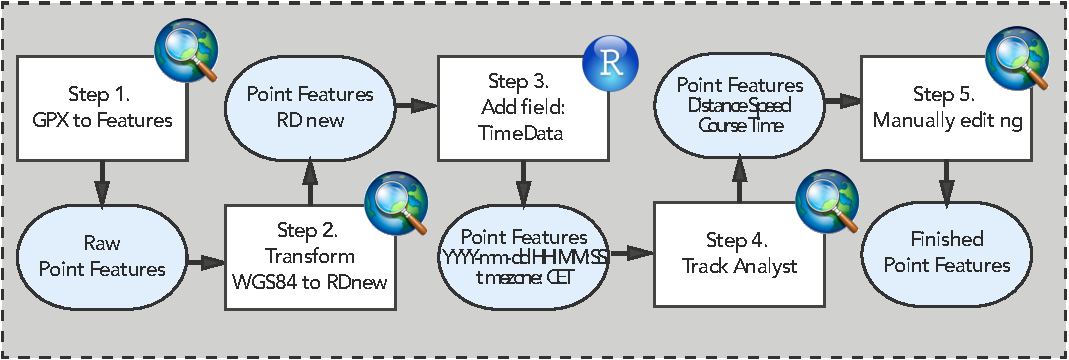
\includegraphics[width=\textwidth]{img/M_preprocessingGPS.pdf}
\centering
\caption{GPS pre-processing flowchart}
\label{gpspp}
\end{figure}

\subsection{Data Collection - Accelerometer}
We used a Samsung Galaxy Core GT-I8260 smart phone which was available at the conducting faculty. With the application; Accelerometer Physics toolbox accelerometer to extract the 3-axis acceleration data on the X, Y and Z axis and the total acceleration called g-force. Physics Toolbox Accelerometer proved to be the best option for extracting the data, for it is easy to use, can store the data in a csv file, with current clock time, time stamp and saves it on the local storage of the phone. It does not require a constant internet connection, and was free for use. Also no knowledge on any pre-programming to read the sensors was required. Some of the other application alternatives considered are: Accelerometer Monitor from Mobile Tools, Accelerometer Monitor from Keuwlsoft Tools, and the AcMeter. Their specifications and reasons why not used, can be found in Annex \ref{Aapps}. 

During all measurements, the smart phone will always be placed horizontally on the Rollator. This means the $z$-axis is pointing down, and will correlate most with movements up and down. The x-axis will be pointing sideways and the y-axis front and back. Acceleration of walking speed will be seen in the $y$-axis. While turns will be seen in the $x$-axis. See figure ~\ref{setup}.
\begin{figure}[t]
\includegraphics[width=\textwidth]{img/M_RollatorSetup.pdf}
\centering
\caption{ Graphical representation of the direction of the axis of the accelerometer on the rollator. \label{setup}}
\end{figure}


\subsubsection{Application version change}
Several versions of the application were used, as the developer updated the app meanwhile. \footnote{Information provided by Chrystian Vieyra, developer of the Physics Toolbox Applications. In e-mail conversation 26-10-15. }
In September 2015 version 1.2.9 was active. On September 9th the version available was 1.3.6. Though, the smart phones used, were not always attached to the internet, and so version 1.29. was used in the beginning. This resulted into failed experiments for there was no wake lock, which keeps the device awake even if the screen turns off while the record button has been pressed. So the app was put to sleep during the measurements. Test rides on a bike were conducted but the gaps of missing data seemed to happen when large bumps occurred in the road and the conducting researcher kept the screen awake more often by touching the smart-phone more often. 

Later measurements were taken with version 1.3.6 and 1.3.7, which did continue the app measuring when the screen was in sleep mode. The only difference between version 1.3.6 and 1.3.7 is a spelling mistake and the graphic layout of the record button.


\subsection{Data Pre-processing - Accelerometer}
The accelerometer dataset contains the following specifications:
\begin{itemize}
\item Time zone: CET. Same as the smart phone settings. 
\item CSV time stamp: clock time in milliseconds
\item No location
\end{itemize}

The measurements resulted in dataset with per feature :
\begin{equation} 
	F_(i) = [ Time stamp, A_{x}, A_{y}, A_{z}, A_{m}] 
\end{equation}
With $A_{x}$ as the $x-axis$ acceleration
$A_{y}$ as the $y-axis$ acceleration
$A_{z}$ as the $z-axis$ acceleration and
$A_{m}$ as the total acceleration.

The total acceleration or g-force is supplied by the application: It is the total acceleration vector of the 3 axis combined. When tested, the calculated $A_{m}$ is equal to the g-force provided by the application. It will be referred to as $A_{m}$ or total acceleration, for G-force can be a confusing concept. It can be calculated by:

\begin{equation}
A_{m} = \sqrt {{A_{x}}^{2} + {A_{y}}^{2} + {A_{z}}^ {2}}
\end{equation} For each time series $A_{i}$ , with $i = {x, y, z}$ 

With cross correlation between the several features, we can detect which feature best represents the walk characteristics. $A_{m}$ is a representative parameter which includes the gait acceleration (Y-axis), the vertical acceleration (Z-axis) and the lateral acceleration (X-axis). ~\cite{Weiss2014} By doing a cross correlation with the Z-axis and the X and Y axis a similarity between the lateral acceleration, mostly caused by the surface, and the gait acceleration is detected. The cross correlation of the $x$ and $z$ axis is expressed by:

\begin{equation}
Corr_{z,x} = \sum z(n)x(n-1)  %blablabla wat doe ik hiermee? 
\end{equation}

Accelerometer output ranged between the normalized range of -2 to 2. Assumed is that the value of 1 means equal to 1 times the gravitational force: 9.81 $m/s^2$ and the value of 0 means no force pulling, so the sensor is flat. The developer stated, that these normalized values differ per type of smart phone.\footnote{Information provided by Chrystian Vieyra, developer of the Physics Toolbox Applications. In e-mail conversation 26-10-15. }

The application contained several settings, which were not described in the application nor on-line. Therefore some sample test were conducted to gain some basic information about the application values and settings. The application had four record interval settings, Normal, UI, Game and Fast. By placing the phone for a while on the table with the different settings the following information was found about the sample frequency of these settings: 

\renewcommand{\arraystretch}{1.5}

\begin{table}[h]
\caption{Sample frequency of the different settings.}
\label{samfreq}
\centering
\begin{tabular}{|p{91pt}|p{91pt}|p{91pt}|p{91pt}|} 
\hline 
 Setting & Points per sec (exact) & Points per sec (approx.) & Periodicity (1/(points per sec))\\
\hline
NORMAL & 4.6 & 5 &  0.2 \\
UI & 11.9 & 10 & 0.1 \\
GAME & 49.6 & 50 &  0.02 \\
FAST & 99.4 & 100 &  0.01 \\
\hline
\end{tabular}
\end{table}

This means that with an average walking speed of 1.3$m/s$ the distance between the measured points will be, 26$cm$ for NORMAL sample frequency, 13$cm$ for UI, 2.6$cm$ for GAME and 1.3$cm$ for FAST sample frequency. 
For further calculations the setting NORMAL is used. This because an interval of 26 cm seams sufficient and the data set will be not too large in size to handle. 

\subsubsection{Sensor errors}
Because the accelerometer sensor is not calibrated and the quality is unknown, it can contain random errors (caused by the accuracy limit of the measuring instrument) or systemic error (caused by incorrect calibration of the measuring instrument). 
By placing the smart phone flat on a table, laying still for several hours, an indication can be given of the sensors offset. This means the z-axis is pointing down and also contains one time the gravitational force pulling it down. Resulting in numbers around 1. The x and y axis are pointing to the side and front/back. Being flat and resulting in numbers around 0.

The following sensor errors were found with setting NORMAL for every axis:

\renewcommand{\arraystretch}{1.5}
\renewcommand{\tabcolsep}{0.2cm}
\begin{table}[h]
\centering
\caption{Average error per axis. Sample frequency 5 per sec (NORMAL)}
\label{averageerror}
\begin{tabular}{|p{56.6pt}|p{56.6pt}|p{56.6pt}|p{56.6pt}|p{56.6pt}|p{56.6pt}|} 
\hline
\multicolumn{2}{|c|}{SAM 3} & \multicolumn{2}{|c|}{SAM 4} & \multicolumn{2}{|c|}{SAM 5} \\
\hline
\multicolumn{2}{|c|}{Average error from 0} & \multicolumn{2}{|c|}{Average error from 0} & \multicolumn{2}{|c|}{Average error from 0} \\ 
\hline
$\xi_{A_x}$ & -0.04 &$\xi_{A_x}$ & -0.05 &$\xi_{A_x}$ & -0.03 \\
$\xi_{A_y}$ & 0.03 & $\xi_{A_y}$ & 0.06 & $\xi_{A_y}$ & 0.05 \\
$\xi_{A_z}$ & 1.01 & $\xi_{A_z}$ & 1.02 & $\xi_{A_z}$ & 1.03 \\
$\xi_{A_m}$ & 1.02 & $\xi_{A_m}$ & 1.02 & $\xi_{A_m}$ & 1.03 \\
\hline
\end{tabular}
\end{table}

These average errors $\xi_{A_x}$ , $\xi_{A_y}$, $\xi_{A_z}$ and $\xi_{A_m}$ are extracted from all measured Accelerometer time series per smart phone. 

\subsection{Assigning location to accelerometer data with GPS}\label{locationassigning}
For reference, the accelerometer data can be linked to the location by using the time-stamp of the accelerometer and the GPS points. With the time stamp, the first GPS point before and the first GPS point after that time is taken. Because the time difference between the first GPS point and the unknown accelerometer point is known and the speed $(s)$ between the GPS points, the distance$(d)$ and so location$(x,y)$ of the unknown accelerometer point is calculated. 

\begin{figure}[H]
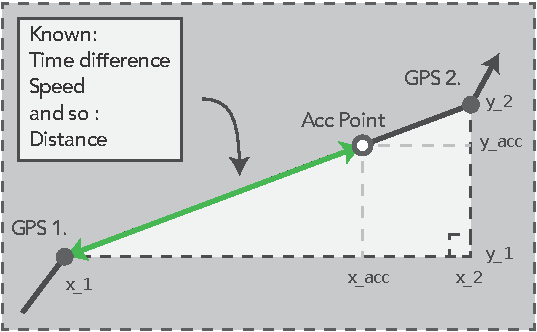
\includegraphics[width=\textwidth]{img/M_location_calc.pdf}
\centering
\caption{Graphical explanation of change point location calculations \label{cpcalc}}
\end{figure}

With coordinates ($x_{1}, y_{1}$) and  ($x_{2}, y_{2}$) in RDnew as the known first and second GPS point, respectively. 

The distance between $(x_{1}, y_{1})$ and $(x_{2}, y_{2})$ is calculated by:
\begin{equation}
d_{1,2} = \sqrt (y_{1}-y_{2})^2 + (x_{1}-x_{2})^2 
\end{equation}

Then, the distance between GPS point 1 $(x_{1}, y_{1})$ and the un-located accelerometer point $(x_{Acc}, y_{Acc})$ is calculated with:
\begin{equation}
d_{1,Acc} = s * time difference((x_{1}, y_{1}) - (x_{Acc}, y_{Acc}))
\end{equation}

The unknown $x$ coordinate of the accelerometer point is calculated with:
\begin{equation}
x_{Acc} = x_{1} +  \frac{d_{1,cp}}{d_{1,2}} * (x_{2} - x_{1})
\end{equation}

And the unknown $y$ coordinate of the accelerometer point is calculated with:
\begin{equation}
y_{Acc} = y_{1} +  \frac{d_{1,cp}}{d_{1,2}} * (y_{2} - y_{1})
\end{equation}

Now we can add the location specific data to the change points, the speed($S$) extracted from the track GPS points and the AHN values, height and slope. Resulting in a feature per observation of:

\begin{multline} 
	F_(i) = [ Time stamp, A_{x}, A_{y}, A_{z}, A_{m}, s, height, slope] 
\end{multline}

\subsection{Data Collection - Movie material}
Most walks were recorded on film, for reference aid. This was done with either a go-pro, flip camera or with the smart phone camera. Pointed at the direct surface in front of the rollator. The images are not used for calculations, solely for reference backup. 

\subsection{Analysis - Mapping irregular surfaces with an Accelerometer}
Several test were conducted with the Measurement Rollator on different surfaces. To see if the vibrations of the rollator are more fierce on surfaces with a more irregular surfaces. Indicating more surface hindrance and so more energy is needed for the rollator user. The assumption is, that the vibrations caused by surface hindrance can be measured through the variance of the z-axis acceleration. We used the Accelerometer (Physics Toolbox version 1.3.7) and the Garmin to record GPS. The goal was to walk with an average walking speed of $4.7 km/h (3.2 – 6.2 km/h)$. This is the walking speed found from literature and own research. Though, while walking it felt quite fast. So the walking speed was kept around 4 km/h as best as possible. The researcher walked herself with the rollator over different surfaces. Each a distance of around $20m$. All the pavement surfaces structures shown in image ~\ref{surfaceimg} were tested. Asphalt or tarmac, brick paving, tiles, gravel, grass and a smooth concrete surface inside was measured. 

\begin{figure}[p]
\includegraphics[width=\textwidth]{img/M_All_surfaces.pdf}
\centering
\caption{Image of every measured surface \label{surfaceimg}}
\end{figure}

\begin{figure}[p]
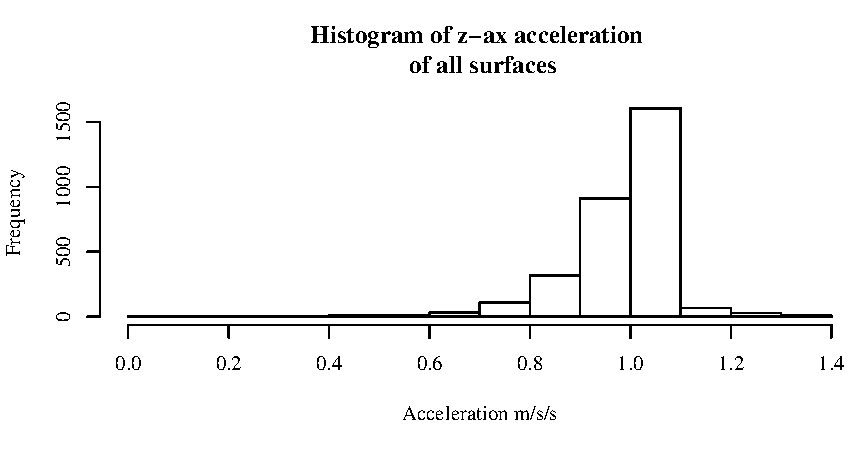
\includegraphics[width=\textwidth]{img/M_Histogram_all_surf.pdf}
\centering
\caption{Histogram of all surfaces $z$-axis acceleration \label{hist}}
\end{figure}



\subsubsection{Statistics}
By providing the descriptive statistics of the accelerometer output as a normal distribution, the differences in the vibrations on different surfaces can be explained. The data is approaching a normal distribution as can be seen in the example histogram of all the surfaces combined.(~\ref{hist}) Vibration goes into both directions so the mean will not show a surface specific outcome and will not differ much between the different surfaces. The means calculated only gave values around the 1. See table~\ref{surfacehindrance} in the results. The variability shows better how rough the surface is. Therefore the variability is used, or the standard deviation together with the 5-number summary to create box plots. Including, the minimum, maximum, median and first and third quantile. To show a better understanding of the effect of the surface on the vibrations on the rollator. The formula for the mean variance and standard deviation:

\textbf{Mean:}  
\begin{equation}
Mean A_{z} = \frac{\sum_{k=1}^n A_{z}}{n}
\end{equation}

\textbf{Variance:}
\begin{equation}
\sigma^2 = \frac{\sum_{k=1}^n (A_{z}- mean(A_{z}))^2}{n-1}
\end{equation}

\textbf{Standard deviation:}
\begin{equation}
\sigma = \sqrt \frac{\sum_{k=1}^n (A_{z}- mean(A_{z}))^2}{n-1}
\end{equation}

\subsubsection{Comparison with Matthews et al. (2003)}
In Matthews et al. (2003)~\cite{Matthews2003} a reference score for hindrance of specific surfaces is provided. Shown in table~\ref{hindrance}.
Small test were conducted measuring surface hindrance for wheelchair users, aiming at surface type and quality for mobility. Six common urban surfaces were tested: concrete, paving, tarmac, brick, grass and gravel. A wheelchair with occupant was pushed down a small ramp the distance rolled provides an measure for rolling resistance. ~\cite{Matthews2003}
These values will be used as a reference, to see if the measured vibrations of the Accelerometer correlate. Because the reference numbers are relative, also the measured outcome is recalculated to a relative factor. Taking the most smooth surface as factor 1 and calculating the rest of the surfaces from this. See results in figure~\ref{comparefig} for a comparison of the values of Matthews and the calculated factors. 
 % figure comparison factors measured and given 4.3

\begin{table}[hb]
\caption[Relative hindrance scores of surfaces]{Relative hindrance scores of surfaces, low scores represent levels of least hindrance ~\cite{Matthews2003} \label{hindrance}}
\centering
\begin{tabular}{|l|l|l|l|l|l|}
	\hline
	Concrete & Paving & Tarmac & Brick & Grass & Gravel\\
	\hline
	1 & 1.2 & 1.3 & 1.6 & 6 & 8 \\
	\hline
\end{tabular}
\end{table}
	\section{Method RQ 4s - Mapping abnormal or change events with changepoint detection using Accelerometer, GPS and AHN2 data}\label{rq2c}

Assuming that in the optimal circumstances, someone will walk with a specific speed in a monotonous way and the pavement has a regular surface, the measured acceleration in the z-axis will show a monotonous pattern. An \emph{abnormal} peak in the continuous data will indicate a problem or obstacle in the pavement surface. Next to this, a sudden change in the walking speed of the person, could indicate a disturbance of the walking route. Together, a sudden drop in speed, plus a peak in the z-axis acceleration, could indicate big bumb or obstacle which causes a change in the walking behaviour of the pedestrian. For example, tackling a curb obstacle with the rollator. 

By looking at the changes or anomalies in the time series data of speed, slope and z-axis acceleration measured during a walk and linking them to location trough GPS measurements, the physical obstacles or hindrances can be located. The changes or anomalies in time-serie data can be determined by the change-point package of R containing specialized change-point finding algorithms for detecting multiple change-points within data and a variety of test statistics.~\cite{changepoint2015, killick2014} A changepoint is the estimation of the point at which the statistical properties(mean or variance) of a sequence of observations changes.

\subsection{The changepoint package}
%the changepoint package and possible methods
The ChangePoint package of Killick et al. 2014 contains functions to detect multiple changes in the mean or the variance of large datasets. First we will explain the concept of change-points and the segment in between. Then, the methods offered by the package will be explained and the possibility to choose different statistical models for penalty fitting. The exact approach of identifying multiple change-points, formulas, methods and references can be found in the report of the changepoint package by Killick et al. 2014~\cite{killick2014}

%changepoints and segments
Having an ordered sequence of data $y_{1:n} = (y_{1}, .... , y_{n})$, a change-point is said to occur within this set when there exists a time, $τ ∈ {1, . . . , n − 1}$, such that the statistical properties of segment ${y_{1}, .... , y_{τ}}$ and segment ${y_{τ+1}, .... , y_{n}}$ are different in some way. Consequently the $m$ change-points will split the data into $m + 1$ segments, with the $i^th$ segment containing data $y_{(τ_{i−1} +1):τ_{i}}$ . Each segment will be summarized by a set of parameters.~\cite{killick2014} Possible is to use the two sides: the change-points $CP_{1:m} = (CP_{1}, .... , CP_{m})$ themselves and the segments $y_{(CP_{i−1} +1):CP_{i}}$ between the change-points. Each, with its own set of parameters. 
The average variance or mean of the segment indicates the homogeneous characteristics of the dataset, between the change-points. 

%possible methods
The Changepoint package implements three multiple change-point algorithms; Binary Segmentation(BS), Segment Neighbourhoods(SN) and the Pruned Exact Linear Time(PELT). Binary Segmentation is an approximate algorithm and most widely used search method. Segment Neighbourhoods has a long computation time but is more exact. PELT is computationally fast and exact. The number of change-points increases linearly as the data set increases. 
In addition the package provides a variety of test statistics for the penalty type settings, for example: BIC, AIC or Hanan-Quinn. 
The penalty settings are used to prevent the model for over fitting and increases the number of parameters in the model to almost always improve the goodness of fit. The default is using no model and taking all measurements into account. When using Asymptotic penalty, the theoretical type I error (0.05) is used. Also a manual penalty can be set, this can be a numeric value or text giving the formula to use. One of the available variables is $n=$length of original data.~\cite{killick2014}

All the different changepoint detection methods had to be tested to see which model approaches the most plausible result and approaches the truth the best. This was shortly done for all individual dataset. Also the best possible penalty settings are considered when there was over or under fitting. We found big difference in characteristics of the dataset for speed, slope and acceleration. Most often the penalty was set manually to $1.5 * log(n)$ to ignore extreme measurements. 

% When over or under-fitting occurs, we adjusted the penalty. Especially in the speed and slope datasets, over-fitting was a problem. Extreme peaks or graduated steps in the speed are due to measurement errors in the GPS. If a model fits too well, these are taken as truth, the penalty settings can even out those extreme measurements. 
% ### Because of overfitting the model of speed a penatlyt type of BIC AIC or Hanan-Quinn can be chosen to solve the problem of overfitting.
% ## a penalty term for the number of parameters in the model; the penalty term is larger in BIC than in AIC.
% ##he penalty discourages overfitting (increasing the number of parameters in the model almost always improves the goodness of the fit).
% ## we use an adjusted penalty to overcome the problem of overfitting. The GPS contains abonormal peaks due to measurement errors. If a model is generated that fits too well, these are taken as truth. Using a penalty these extreme measurments are not taken into the analysis. These are plausibly artifacts of the data rather
% ## than true changes in the underlying process. In an effort to remove these seemingly spurious changepoints we can increase the penalty to 
% ## The result seem more plausible. 

\subsection{Routes measured}
For testing if the change-point method is usable for detecting obstacles while walking, several test were walked, during the RollatorLoop 2015.
We used the Garmin Summit for the participants and the Leica system on the Meetrollator. 3 smart phones with the Accelerometer (Physics Toolbox version 1.2.9) were used. Here all the accelerometer measurements failed because or the wrong application version. See Annex \ref{Afailed} for the measured tracks and the accelerometer output. Eventually, the measurement with the Leica system could be used for analysing speed and slope. But the accelerometer was left out here. Also, half way the route, the Leica system stopped measuring. See figure \ref{leicatracks} for the route.
So, secondly a bike ride was monitored for testing the application settings again, with the Accelerometer (Physics Toolbox version 1.3.7) and the GPS Geotracker Application to record GPS. When this seemed to work, also a walk with the measurement rollator was conducted by the researcher herself. Using the Accelerometer (Physics Toolbox version 1.3.7) and the Garmin Summit. Both tracks are shown in figure \ref{tracks}.

\begin{figure}[hb]
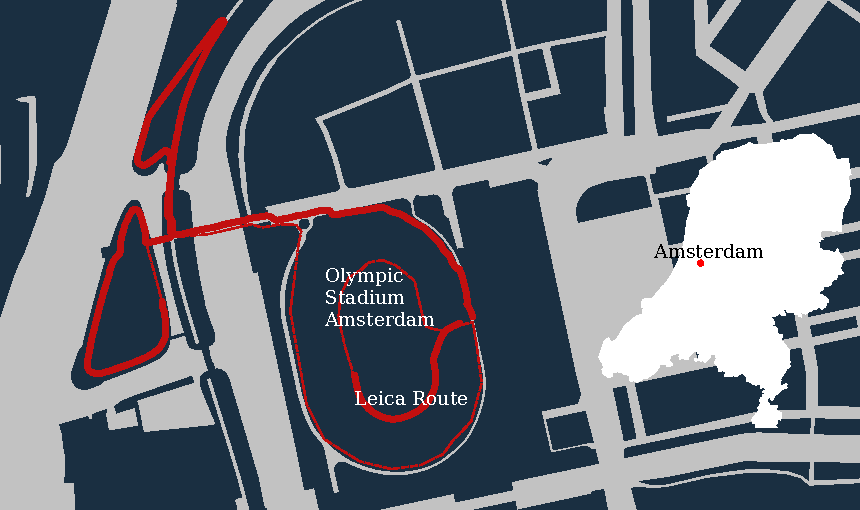
\includegraphics[width=\textwidth]{img/M_overviewRouteLeica.pdf}
\centering
\caption{ Map of Leica route in Amsterdam\label{leicatracks}}
\end{figure}

The datasets of the accelerometer are combined with the location dataset of the GPS measurements. The location assigning is done with the same method as described in the previous section \ref{locationassigning}. The location specific data was added to the dataset: the speed($S$) extracted from the GPS points and the AHN2 values, height and slope. Resulting in a feature per observation of:

\begin{equation} 
	F_{(t)} = [ A_{x}, A_{y}, A_{z}, A_{m}, s, height, slope] 
\end{equation}

The dataset per route was approached as a time-series dataset to applying the changepoint method. Each route and data range on the route had its own specific settings to get the best model of fit. Eventually this resulted in a changepoint feature for every $m^{th}$ changepoint observation:

\begin{equation}
CP_{m} = [ breakpoint index, mean, variance, time, x,y]
\end{equation}
This is applicable to the acceleration, speed, slope and height. The change-points are detected with the variance setting for the acceleration and mean for change-points detection for speed, height and slope: 

$CP_{mean(s)}, CP_{Var(A_{z})}, CP_{Var(A_{m})}$ and $CP_{mean Height}, CP_{mean slope}$ 

With all change-points having location coordinates($x,y$) in RD new and a time stamp. When plotting all changepoints on the map patterns in the route can be visually detected.

\begin{figure}[ht]
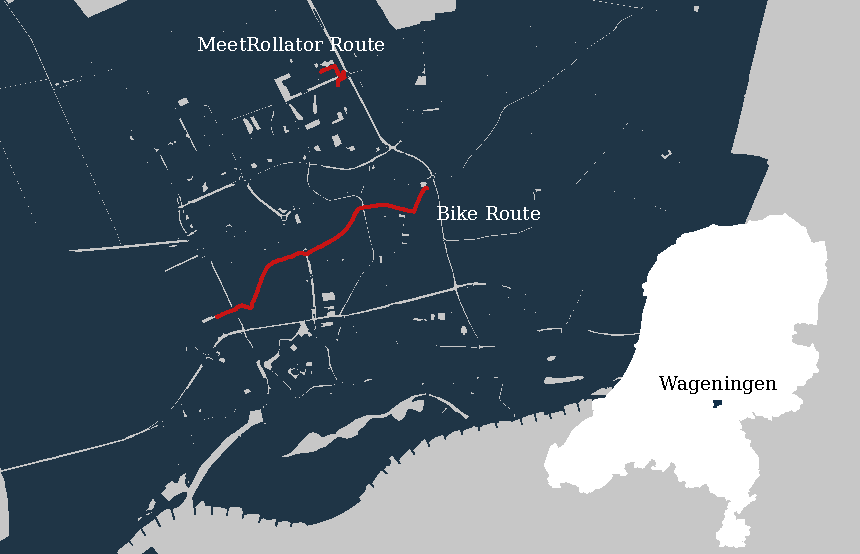
\includegraphics[width=\textwidth]{img/M_overviewRoute.pdf}
\centering
\caption{ Map of tracks measured in Wageningen\label{tracks}}
\end{figure}


	


\section{Mapping irregular surfaces with an Accelerometer}
\begin{description}
\item[Hypotheses 1] : Vibrations of the Rollator increase while walking on surfaces with more hindrance. 
\item[Hypothesis 2] : The vibrations caused by the hindrance can be measured with the variance in the z-axis acceleration. 
\end{description}

Several test were conducted with the Measurement Rollator on different surfaces. Used the Accelerometer (Physics Toolbox version 1.3.7) and the Garmin to record GPS. The goal was to walk with an average walking speed of 4.7 km/h (3.2 – 6.2 km/h). This is the walking speed found from literature and own research. Though, while walking it felt quite fast. So the walking speed was kept around 4 km/h as best as possible. The researcher walked herself with the rollator over different surfaces. Each a distance of around 20 m. 

\subsubsection{Set-up}
The smart phone will always be placed horizontally on the Rollator. This means the z-axis is pointing down, and will correlate most with movements up and down. The x-axis will be pointing sideways and the y-axis front and back. Acceleration of walking speed will be seen in the y-axis. While turns will be seen in the x-axis. See figure ~\ref{setup} and ~\ref{setup2}

\begin{figure}[h]
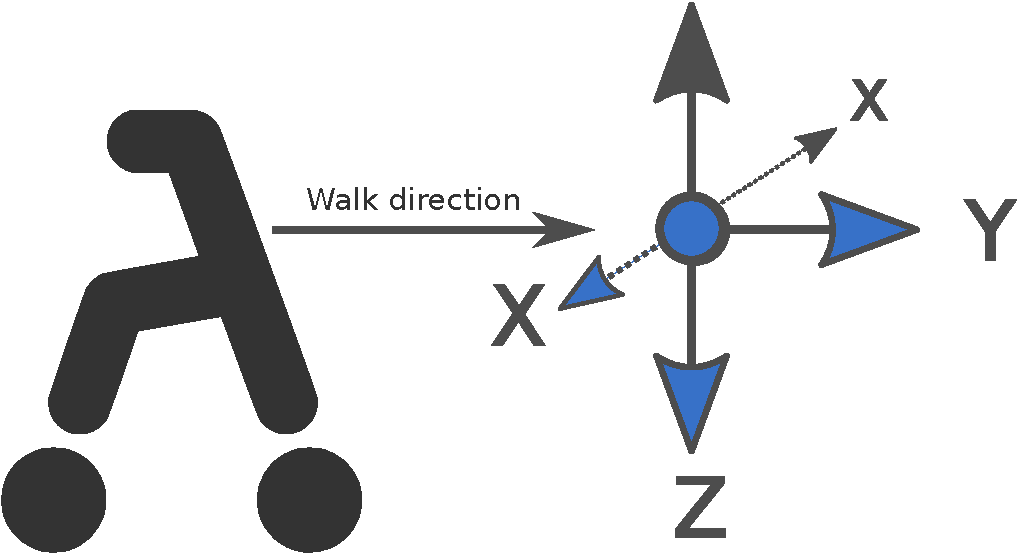
\includegraphics[width=0.5\textwidth]{img/M_rollator_setup.pdf}
\centering
\caption{ Graphical representation of the direction of the axis of the accelerometer on the rollator. \label{setup}}
\end{figure}

\begin{figure}[h]
\includegraphics[width=0.5\textwidth]{img/M_setup}
\centering
\caption{ Set-up of smart phone attached to the measurement Rollator. \label{setup2}}
\end{figure}

All the pavement surfaces structures shown in image ~\ref{surfaceimg} were tested. Asphalt or tarmac, brick paving, tiles, gravel and grass. Also a smooth concrete surface inside was measured. 

\begin{figure}[h]
\includegraphics[width=0.7\textwidth]{img/M_all_surfaces}
\centering
\caption{Image of every measured surface \label{surfaceimg}}
\end{figure}
\clearpage

\subsection{Statistics}
By providing the descriptive statistics of the accelerometer output as a normal distribution, the differences in the vibrations on different surfaces can be explained. The data is approaching a normal distribution as can be seen in the example histogram or tarmac.(~\ref{hist})
\begin{figure}[!h]
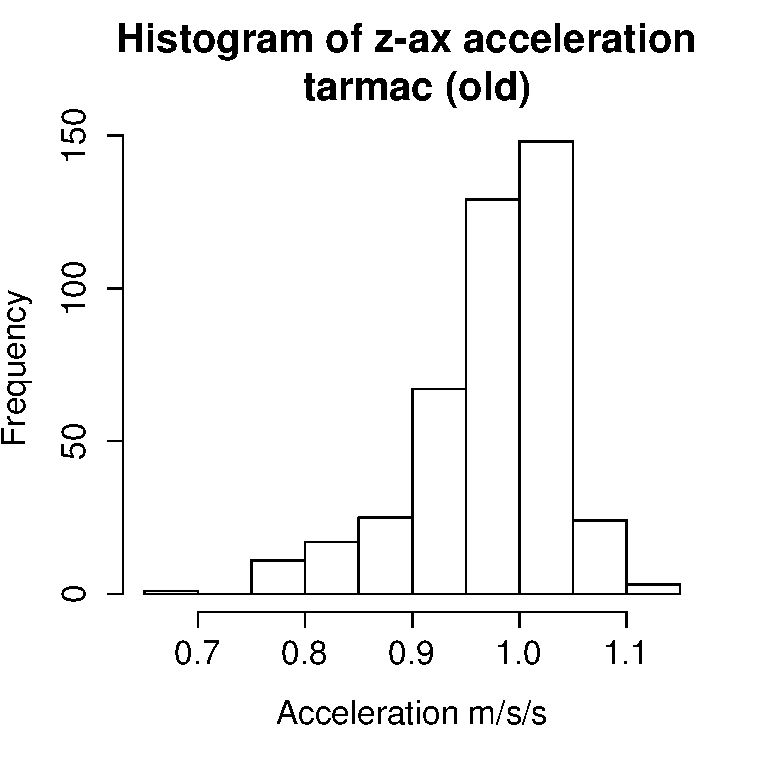
\includegraphics[width=0.5\textwidth]{img/M_hist_tarmac_old.pdf}
\centering
\caption{Histogram of tarmac surface z-ax acceleration \label{hist}}
\end{figure}

Vibration goes into both directions so the mean will not show a surface specific outcome and will not differ much between the different surfaces. The means calculated only gave values around the 1. See table~\ref{stathindrance}.
% 4.3 statistic summary surface hindrance in results

The variability shows better how rouch the surface is. Therefore the variability is used, or the standard deviation together with the 5-number summary to create box plots. Including, the minimum, maximum, median and first and third quantile. To show a better understanding of the effect of the surface on the vibrations on the rollator. The formula for the mean variance and standard deviation:

\textbf{Mean:}  
\begin{equation}
Mean A_{z} = \frac{\sum_{k=1}^n A_{z}}{n}
\end{equation}

\textbf{Variance:}
\begin{equation}
\sigma^2 = \frac{\sum_{k=1}^n (A_{z}- mean(A_{z}))^2}{n-1}
\end{equation}

\textbf{Standard deviation:}
\begin{equation}
\sigma = \sqrt \frac{\sum_{k=1}^n (A_{z}- mean(A_{z}))^2}{n-1}
\end{equation}

\subsection{Comparison with Matthews et al. (2003)}
In Matthews et al. (2003)~\cite{Matthews2003} a reference score for hindrance of specific surfaces is provided. Shown in table~\ref{hindrance}. These values will be used as a reference, to see if the measured vibrations of the Accelerometer correlate. Because the reference numbers are relative, also the measured outcome is recalculated to a relative factor. Taking the most smooth surface as factor 1 and calculating the rest of the surfaces from this. See results in figure~\ref{comparefig} for a comparison of the values of Matthews and the calculated factors. 
 % figure comparison factors measured and given 4.3

\begin{table}[h]
\caption[Relative hindrance scores of surfaces]{Relative hindrance scores of surfaces, low scores represent levels of least hindrance ~\cite{Matthews2003} \label{hindrance}}
\centering
\begin{tabular}{|l|l|l|l|l|l|}
	\hline
	Concrete & Paving & Tarmac & Brick & Grass & Gravel\\
	\hline
	1 & 1.2 & 1.3 & 1.6 & 6 & 8 \\
	\hline
\end{tabular}
\end{table}

\section{Mapping abnormal or change events with change point detection using Accelerometer, GPS and AHN2 data}

Assuming that in the optimal circumstances, someone will walk with a specific speed in a monotonous way. Then, an \emph{abnormal} event in continuous data will indicate a problem or obstacle. 

\begin{description}
\item[Hypotheses 1] : Obstacles, curbs or bumps cause a sudden change in the walking behaviour and so can be seen by analysing the accelerometer and GPS time series and filtering out abnormal events in the time series.  
\item[Criteria]: 
\begin{itemize}
\item Sudden drop in speed.
\item Large change in all 3 axis of accelerometer or total acceleration. 
\item Sudden increase or change in slope or curvature. 
\end{itemize}
\end{description}

Going from one kind of surface to another will show a change in the vibrations. Also walking over a bump will show an abnormal peak in the measured acceleration. These changes in the vibrations of the axes can be determined by the change-point package of R containing specialized change-point finding algorithms for detecting multiple change-points within data and a variety of test statistics.~\cite{changepoint2015,  killick2014} 

The package contains functions to detect changes in the mean or the variance of the data. A change point is the estimation of the point at which the statistical properties of a sequence of observations changes. Having an ordered sequence of data $y_{1:n} = (y_{1}, .... , y_{n})$, a change-point is said to occur within this set when there exists a time, $τ ∈ {1, . . . , n − 1}$,such that the statistical properties of segment ${y_{1}, .... , y_{τ}}$ and segment ${y_{τ+1}, .... , y_{n}}$ are different in some way. Consequently the $m$ change-points will split the data into $m + 1$ segments, with the $i$th segment containing data $y_{(τ_{i−1} +1):τ_{i}}$ . Each segment will be summarized by a set of parameters.~\cite{killick2014}

% changing $y$ to $f$ for better distinction between y ax and data range ?



The changepoint package implements three multiple change-point algorithms; Binary Segmentation, Segment Neighbourhoods and the exact linear time, PELT. Binary Segmentation is an approximate algorithm and most widely used search method. Segment Neighbourhoods has a long computation time but is more exact. PELT is computationally fast and exact. The number of change-points increases linearly as the data set increases. The exact approach of identifying multiple change-points, formulas, methods and references can be found in~\cite{killick2014}

	
For this research the 2 sides of the change points are used; the change-points $CP_{1:m} = (CP_{1}, .... , CP_{m})$ themselves and the segments $y_{(CP_{i−1} +1):CP_{i}}$ between the change-points, eacht, with its set of parameters. For the vibrations measured by the accelerometer, the change-points indicate an abnormal event while the segments between the change-points indicate a phase of monotonous movement or monotonous surface. 


For the accelerometer data always has the mean around the same number, the degree of hindrance or occurrence of an obstacle, will show more in the variance of the data. 


The changes are detected using the exact multiple change-point method (PELT or SegNeigh) or approximate (BinSeg) methods. ~\cite{changepoint2015}\newline

For testing if the change-point method is usable for detecting obstacles while walking, a bike ride was monitored and a walk with the measurement rollator. 
Several more test were walked, during the RollatorLoop 2015, but these measurements failed. See Annex \ref{} for the measured tracks and the accelerometer output. 

The tracks measured with the geoTracker application and the Accelerometer application on the smart phone which did succeeded are shown in figure \ref{tracks}. 

\begin{figure}[h]
\includegraphics[width=\textwidth]{img/M_map_routes.pdf}
\centering
\caption{ Map of both tracks used \label{tracks}}
\end{figure}

\subsection{Segments between changepoints}
The average variance of the segment indicates the surface characteristics. If combined with the location, the values indicate characteristics of the walk and walk changes. Even the location specific characteristics can be extracted to the time-series observations.

The feature vector for every $ith$  observation for the 3-axis signal is represented by:

\begin{equation}
F_{xyz}(i) = [ x, y, z, A_{m}, Var(A_{z}), Var(A_{m})]  %% and all other stuff needed. 
\end{equation}

To this we could add the average variance per segment between the change-points:

\begin{equation}
F_{xyz}(seg) = [Var(A_{z}), Var(A_{m})]
\end{equation}

For reference, the change-points are linked to the location by using the time-stamp of the accelerometer and the GPS points. With the time stamp, the first GPS point before and the first GPS point after that time is taken. Because the time difference between the first GPS point and the change point is known and the speed between the GPS points $(s)$, the distance and so location of the change point is calculated. 

\begin{figure}[h]
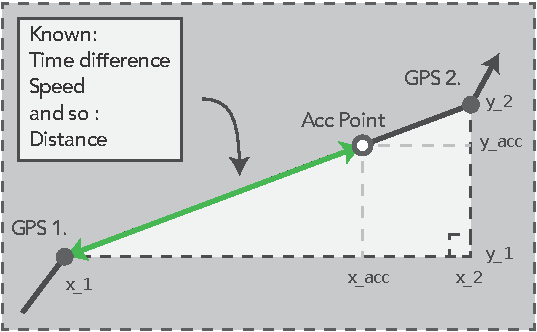
\includegraphics[width=0.75\textwidth]{img/M_location_calc.pdf}
\centering
\caption{Graphical explanation of change point location calculations \label{cpcalc}}
\end{figure}

With coordinates ($x_{1}, y_{1}$) and  ($x_{2}, y_{2}$) in RDnew as the known first and second GPS point, respectively. 

Distance between $(x_{1}, y_{1})(x_{2}, y_{2})$:
\begin{equation}
d_{1,2} = \sqrt (y_{1}-y_{2})^2 + (x_{1}-x_{2})^2 
\end{equation}

Distance between $(x_{1}, y_{1})(x_{cp}, y_{cp})$:
\begin{equation}
d_{1,cp} = s * time difference((x_{1}, y_{1}) - (x_{cp}, y_{cp}))
\end{equation}

New $x$ coordinate:
\begin{equation}
x_{cp} = x_{1} +  \frac{d_{1,cp}}{d_{1,2}} * (x_{2} - x_{1})
\end{equation}

New $y$ coordinate:
\begin{equation}
y_{cp} = y_{1} +  \frac{d_{1,cp}}{d_{1,2}} * (y_{2} - y_{1})
\end{equation}


Now we can also add the location specific data to the accelerometer segments, the speed($S$) extracted from the track GPS points and the AHN values, height, slope and curvature. Resulting in a feature per observation of:


\begin{multline} 
\centering
	\begin{equation*} F_{xyz}(i) = \end{equation*}
	\\
	\begin{equation*}[ A_{x}, A_{y}, A_{z}, A_{m}, Var(A_{z}), Var(A_{m}), \end{equation*}
	\\
	\begin{equation} Var(A_{z seg}), Var(A_{mseg}) , s, height, slope, curvature ] \end{equation}
\end{multline}

And the average values for the segments between the change-points:

\begin{equation} 
F_{xyz}(seg) = [ Var(A_{z}), Var(A_{m}), Var(A_{z seg}), Var(A_{mseg}) , A_s, A_height, A_slope, A_curvature ] 
\end{equation}

With cross correlation between the several features, we can detect which feature best represents the walk characteristics. 

By doing a cross correlation with the Z-axis and the X and Y axis a similarity between the lateral acceleration, mostly caused by the surface, and the gait acceleration is detected. The cross correlation:

\begin{equation}
Corr_{z,x} = \sum z(n)x(n-1)  %blablabla wat doe ik hiermee? 
\end{equation}

\subsection{Comparing change-points}
The change-points detected in the accelerometer data can be compared against change-points that occur in the speed time-series of the height data. 
First the change-points are detected with the variance and mean change-points detection for speed, height, slope and curvature. The time difference or the distance difference indicates how close the change-points are to each other. If the change-points are close it indicates an abnormal event in multiple data sources, which could indicates an obstacle. 

So there are change points in the accelerometer, speed, and AHN data: $CP_{mean(s)}, CP_{Var(s)}, CP_{Var(A_{z})}, CP_{Var(A_{m})}, CP_{Height}, CP_{slope}$ and $CP_{curvature}$. With all change-points having location coordinates($x,y$) in RD new and a time stamp. 

% Distance to the closest point location. RMSE? maybe? RMSE of the distances between the points. 

	\chapter{Conclusion and discussion} 
The first section of this final chapter restates the research questions and presents the main conclusions of this research. Section 5.2 discusses the results outcomes and limitations of the research. Section 5.3 gives several recommendations to improve this research and for possible future research.

\section{Conclusion} %antwoord op vragen geven
The objective of this research was to get the critical walkability factors that elderly experience while walking outdoors with a rollator, and explore the possibilities of geo-data and GIS analysis to visualize them, to raise more awareness and shed more light on the forgotten elderly pedestrian. This to trigger possible action at decentralized governments for increasing walking activity of elderly people. Consequently this may support health, the capability to live independently and grow old in their own house and environment. All may contribute to less need for healthcare and so reducing costs for elder care and improving the overall quality of life. 

In order to analyse and map the critical walkability factors for elderly people depended on a rollator, in the urban outdoor space, the following sub-objectives and research questions were developed:
\begin{enumerate}
\item Find the critical factors for walkability in the urban outdoor environment for elderly depended on a rollator.
\item Map and analyse these critical factors, 
 \begin{enumerate}
 	\item by analysing existing and available geo-data and testing its suitability and detail required
 	\item by collecting geodata (measuring rollator movements with an accelerometer) and analysis
 	\item by comparing these the two data sources (by using the change point method) 
 \end{enumerate}
\end{enumerate}

% restate the research question. nr 1. Critical walkability factors
To find the critical walkability factors or urban outdoor environment for elderly people, with a rollator a literature study was conducted and interviews were held. This showed that there are many criteria mentionable to improve on for the elderly pedestrian. The top 3 of critical walkability factors were, wrongly parked bikes and cars, irregular cobbled surfaces and sloping pavements. The small part of interviews held with rollator users, underline the importance of the quality of the pedestrian area. The most important thing mentioned is, that, when surfaces will be more smooth, and surroundings less exhausting, longer and more comfortable walks will be able. Also confirmed is that the older peoples' perceived needs as pedestrian in the outdoor urban environment are considered important by the older people themselves. This research found walkability factors in line with previous researches and contributes to the knowledge specifically for Amsterdam. From the final list of critical factors assembled by all the findings, one of the main irritations specifically for Amsterdam are wrongly parked bikes and cars. Mainly due to the small pavement areas and parking on the pavements. Many road users, hardly think about the less impaired road users while parking their bike outside, against a lantern pole, and so blocking the pavements for wheelchair or rollator users. Next to this, research into the policy design and interviews with the municipality showed that policy design, does not take pedestrians into account sufficiently. Let alone, the elderly or mobile impaired pedestrian. 


% restate the research question. nr 2. Mapping the Critical walkability factors
In order to map and analyse these critical factors, the first step was to analyse existing geo-data and test the detail required. Only the work Matthews et al. (2003), Modelling Access with GIS in Urban Systems~\cite{Matthews2003}, Svensson (2010)~\cite{Svensson2010} and Duncan et al. (2011) with Walk Score: Estimating Neighbourhood Walkability~\cite{Duncan2011} provide methods for quantifying walkability factors in a GIS system. They use a multi-criteria model with quantitative and qualitative techniques to make visible how the build environment can be hostile for the mobile impaired. 
For this research only a few datasets were used. The GBKA and the AHN2. An attempt was made to collect data on the location of curbs, ramps, what the material of the surface is etc. Though, there is no indication in the available data-sets of Amsterdam whatsoever on where curbs are located, how high they are, and whether there are ramps placed or where the curb is lowered. Besides this, no information could be found about the exact type of material of the surface or maintenance activities. Only an overview map showing material use per neighbourhood is available, see the Puccini map in annex \ref{pucciniMap} 

% The critical factors derived from the available geo-data is sloping surface and the amount of area available for pedestrians. 
The first step was to determine the pedestrian area with the available GBKA and have a look at is general characteristics and quality. A new approach had to be invented, as Matthews et al. did, for no label was attached with which target group the dedicated polygon belongs to. A small pilot study was held for the Jordaan in Amsterdam to see its suitability. The own approach to determine which areas are pedestrian area, showed rather high numbers for pedestrians. Around 53\% of the public space in the test area Jordaan, belonged to pedestrians. A surprising amount as often in Amsterdam, pedestrians pavements are very narrow. This did however, include parking plots and public squares and the calculated area contains a lot of poles, bike racks, traffic signs or any other object placed on the pavement. The approach showed that an automatic approach is hard for classifying the polygons, and many mistakes are made in the data set. 

% The most mentioned critical walkability indicators which are researchable with GIS methods are sloping pavements
Secondly, the AHN2 was used to derive sloping pavements above 4\% slope. A lot of roads, classified for motorized transport showed average values below the 4\% slope, while many pedestrian classified areas, had a slope higher then 4\%. In numbers, the allowable 4\% of slope for pedestrian pavement reduced the optimal pedestrian area to only 8\%. Showing a lot of area being too steep for pedestrian allowable limits. While roads, for motorized transportation have less steep slopes, around 38\% is below the 4\% slope. 

In conclusion, the GBKA showed that in the available geo-data of the municipality, still lacks detail and is insufficient for quick pedestrian analysis as the pedestrians are forgotten. This confirms the statements of the introduction, that pedestrians are forgotten in data. Only the AHN2 promises good usage for pavement analysis as it gives good insight in the sloping pavements and is detailed enough to detect curbs. 

The collection of own data is done by measuring rollator movements whit an accelerometer. 
Works from Weiss et al. 2014 and Wang et al. 2015 gave the inspiration to work with the concept of a Smart Walker. Several test routes were walked during the rollator loop. These, unfortunately failed to measure the accelerometer sensor and were not usable. Other tests, walking the rollator myself and measuring different surfaces, showed that irregular surfaces can be measured with a accelerometer. The different kind of surfaces showed clear distinctions in the amount of vibrations when looking at the variance over the measured track. With grass and stones having the highest variance and vibrations and smooth concrete the lowest. When comparing this to a research done by Matthews et al. (2003) a correlation of 0.72 is found. Indicating the two studies do correlate but not highly. This, because the surfaces of Matthews and this research were probably not the exact same, what was measured differs and measurement methods differ. Matthews measured surface hindrance as the accelerometer measures the vibration effect on the rollator. Though, a correlation exist between vibration of the rollator and surface hindrance. And that surface hindrance can be approached with an accelerometer as well. 

In order to compare both methods, using existing geo data to map walkability factors and comparing and testing them with a Smart Walker, a change point analysis was used. the change point method shows an interesting concept for detecting obstacles during a walking route. Several locations can be indicated where the walking behaviour (speed), the slope of the location, and the accelerometer behaviour fall together as expected, a large obstacle is detected. Also some peaks in the acceleration of the z-axis are located around imperfections in the pavement and are not accompanied by speed changes, indicating a small obstacle. Though, breaks and stops by the participant are also included. Several interesting events in the walking routes are that almost all change points for speed, in the Leica route, can be explained through logical reasoning. 
Also the change points in the z-axis acceleration in the walking route with the MeetRollator seem to be related to the true situation. This however, cannot be stated definitively as here the GPS performed poorly and so the points cannot be accurately compared to the location. Overall, the most change points in the z-axis acceleration occur where obstacles are taken, the route is started or ended. On the larger straight segments of the route, where the pavement stays nearly the same and walking speed is continuous, less change points can be found. The big amount of wrong points in the slope change points, actually originate from the inaccurate location determination and resulted in extracting values form the slope raster at the wrong location. Hopefully, we can add obstacle detection and surface quality monitoring as another possible application to the Smart Walker, next to fall protection, early warning systems, health monitoring, navigation help or cognitive assistance.


\section{Discussion} %bevestiging tov literatuur
 

\subsection{The forgotten pedestrian}
When policy design documents and the contacts from the municipality state that the pedestrian area is often the residual area in design and has the least priority, the arguments from the introduction are confirmed, that indeed, the pedestrian is forgotten in design. Moreover, this applies for the total group of pedestrians, not specifically for the mobility impaired pedestrians, who even require a more well designed public space. 

Also the forgotten pedestrian in data is confirmed. Not only the PQN report states that there is not enough data on pedestrians~\cite{Sauter2010}, also Matthews et al. (2003)~\cite{Matthews2003} encounters the first main problem, that no data is held on pavement centrelines. The basic layer for a GIS model is to know, what is pedestrian area or not. Our own research, confirmed that the GBKA, the most detailed topology dataset of the municipality of Amsterdam, did indeed, contain no label on whether it was a road for cars or a pavement for pedestrians. Through a own set up analysis of general assumptions a approximation to label the polygons was conducted. This, seemed more difficult then expected. Matthews stated that precise pedestrian routes can be mapped manually.~\cite{Matthews2003}


\subsection{Interviews with elderly}

As Stahl et al. 2008 stated, user involvement leads to research of grater relevance to people and the findings more likely to be implemented.~\cite{Stahl2008} Their research is all based on the problems identified by elderly people and therefore of great relevance. Also for this study the involvement of elderly with a rollator was perceived as important. For the conducting researcher to be young and not having any experiences with mobility problems, it was key to hear from first hand. The first intention was to interview at least 20 elderly in Amsterdam, that walk outside regularly with a rollator. Unfortunately, this seemed harder then firstly assumed. Elderly care houses were not keen on cooperating. Calling would often result into a redirection to the location manager and no answer to the e-mails. Some institutions did show some enthusiasm. The Flessenoord and .. were willing to cooperate, but could only provide 3 participants who walked outside with the rollator. One participant was not available in the end. The Buurtzorg Centrum were also enthusiastic. After several calls and e-mails, they never responded with possible contacts for participants. In the end the short interviews at the Rollatorloop gave a bit more insight. Though, these interviews were conducted rather quickly without any control system.

The participants that did answer already showed how strong the influence of the personal preferences has on the perception to its surroundings. One of the participant really likes walking while the other rather stays inside. This strongly influenced their feelings and emotions they had to walking outside. Through this we can say there is a lot of differences in rollator users. Perception of safety is different for every individual. Very personal determinants. 


When going to the Rollatorloop, noticed was that there are a lot of different rollators. This research did not take into account the different type of rollators available. Thought, the type of wheels and structure of frame might really influence the measurements and can result in different data characteristics.

% ?Safety, robbery and perception of safety are hard to classify (hang jeugd)


\subsection{The Accelerometer sensor}
The application, Physics Toolbox Accelerometer, was a good application and easy to use for measure the accelerometer sensor of the phone. However, the first versions of the application made the app stop measuring when the phone went in sleeping mode. The test rides done on the bike could have been done better. Also the exploration of the test data was too quick and roughly done for the researcher was not familiar with these kind of datasets. A better planning of experiments was needed, and a more clear focus in the first stage of the experiments was lacking. The overall time planning was weak. After a more in depth research into the application behaviour and settings and contacting the developer, more controlled knowledge was gathered about the working of the application. Now, after the application version change and the improvement of the application, it is perfect for using it in this kind of research. If more time was available, again elderly could have been contacted to do the same kind of measurements again. With the Leica and a good working accelerometer application. 

The accuracy or errors from the accelerometer are unknown, as the quality of the sensor in the phone is unknown and not researched. Also the exact meaning of the application values are unknown. These could not be tested, as no good reference accelerometer sensor was available. Overall the outcome of the measurements seemed quite credible. Also the tests with putting the accelerometer flat on the table, did not show any weird peaks or deviations. 


\subsection{Influenced experiments}
After the failed measurements, the researcher herself conducted some extra walks. This could give a wrong image on the measured walking behaviour outcome. From Wang et al. we learned that there is no difference in walking gait characteristics between elderly and young people.~\cite{Wang2015} But that elderly are more used to handling a rollator compared to young people, for which a rollator could be an obstacle in moving more easily. Walking with the rollator myself could have influenced the outcomes. 

\subsection{Spatial accuracy, detail is key}
The location measured with the smart phone  or the Garmin summit are not exact enough to detect the location on a few centimetres exact. This resulted in wrong extraction of data values from the AHN2 and the slope raster. The detected change points from this dataset did not represent the true values for the location were the route was walked. Therefore many slope change points cannot be used to form a conclusion. In order to detect exactly where a route was walked, a good location determination is needed. The detail required, is almost on stone level. It has no use when it cannot be determined if someone is walking on the right side of the street or the left. Also on the pavement section, even put holes or curbs are of significant importance. The Leica system can detect the location on a few centimetres accuracy. But is a heavy system which cannot be easily mounted on a rollator without influencing the rollator control and movement. Possibly, causing a dangerous situation for the elderly depending on it. 

\subsection{Changepoint method}
Unknown method, which not used before. Though shows a lot of potential and interesting opportunities to analyse statistical route characteristics. 

The urban environment will never be optimal, so certain change points will indicate not so important happenings. 

deviations in the measurements:
starten met lopen, is een harde duw tegen de rollator? waardoor er een piek in de accelerometer data ontstaat. 


Could not use trend, seasonality and random analysis, for no seasonality in the data. Surface hindrance changes per surface. Obstacles show more as abnormalities. BFASTt method. BFAST, Breaks For Additive Season and Trend, integrates the decomposition of time series into trend, season, and remainder components with methods for detecting and characterizing change within time series. BFAST & BFASTmonitor: http://bfast.r-forge.r-project.org/ 



\section{Recommendations} %hoe nu verder. Wat meer? LIJST
Recommendations to improve this study
\begin{itemize}
\item Conduct more interviews with elderly living in Amsterdam and walking with a rollator outdoors, to get a better understanding of the location specific problems. Though, trough the literature research and the few interviews held, already a good insight is presented. 

\item In order to conduct a goo pedestrian area classification, it would have been better not to include parking plots into the pedestrian area. Comparing the classification methods with manual classification could have said more about the accuracy of the method. But was too time consuming for this research. 

\item Conduct more controlled experiments with elderly themselves. Also comparing routes walked in a controlled environment against routes walked in the real living environment. This can give better insights if this methods works for detecting obstacles along the real walking routes of elderly, when walked by themselves. Instead of a young vital person walking with a rollator. 

\item Use better GPS systems, like the Leica system for location determination. The detail for which the detection of obstacles is needed, has to be very precise. The slightest deviation can give falsehoods in the change point detection for slope. The research of Wang et al.~\cite{Wang2015} uses exact accelerometer to monitor the displacement for every step made. By using this method the route of a person could be exactly determined from the starting point, with an accuracy of about 1 cm and no GPS would be needed. This would also require a standard measure rollator were the exact distances of the sensor to the wheels and frame has to be known.

\item The AHN2 promised good possibilities to detect surface quality and sloping pavements. Even the detection of curbs and ramps could be possible. More research to the application and possibilities of the AHN2 can be interesting.
\end{itemize}
Recommendations for future research:
\begin{itemize}
\item Find a possible way to quantify the relation between surface hindrance and the effort needed for elderly with a rollator to walk on. For example measuring energy use of elderly. Also the perception of elderly to different surface circumstances could be measured. An interesting link could be the report from Hogertz et al. 2010~\cite{Sauter2010}, which tries to measure skin conductivity as a quantitative measure for arousal. 

% \begin{figure}
% \includegraphics{img/D_hogertz}
% \end{figure}

Possible applications of smart phone with accelerometer use, for measuring rollator movements or surface resistance. Translate this to the amount of energy that elderly consume. 

\item Possible applications might be to detect the kind of surface material from the accelerometer signatures. Create a specific signature for a specific surface material. What has to be taken into account is the different set of rollators that exists. Which react differently to surface irregularities.

\item This study could be used to create a low cost, non-intrusive method for identifying the location of obstacles on the route of elderly with a rollator. A more in detail method could be designed, that automatically filters out priority obstacles where the data changes in a specific way. 

\item using the change point method and regarding a route as a time series dataset could be an interesting method to detect walking behaviour, driving behaviour changes. 

\item Detecting wrongly parked bikes and cars. or raise more awareness under citizens about the problems they cause when parking their bikes wrong. I noticed I never thought about the placement of my bike in relation to the rest of the pavement until I started this project. It makes you look with different eyes and makes you more aware of were to park your bike so enough space is left for others to pass through.  

\end{itemize}






\section{Final words}

It is proven that for elderly, who are more vulnerable, environmental attributes can be barriers to an active engagement in urban life. The quality of the immediate environment is a significant determinant of elders well-being, independence and quality of life. Developing ways to quantify their problems and add more data on their walkability quality could lead to more insight and hopefully to interventions on pavement level. In the near future, there will be more elderly who are willing to live independently and grow old in their own home. In order to facilitate this, we have to look forward and adapt the environment now when we are still young. 









 

 
	% \chapter[Discussion and conclusions]{Discussion and conclusions} 
%  restate the research question. nr 1. Critical walkability factors
The critical walkability factors for urban outdoor environment for elderly people, with a rollator, show that there are many things mentionable to improve on, and policy does not take pedestrians into account sufficiently. When policy design documents and the contacts from the municipality state that the pedestrian area is often the residual area in design and has the least priority, the arguments from the introduction are confirmed, that indeed, the pedestrian is forgotten in design. Moreover, till so far this applies for the total group of pedestrians, not, the mobility impaired pedestrians, who more require a well designed public space. 

The small part of interviews held with rollator users, underline the importance of the quality of the pedestrian area. When surfaces will be more smooth, and surroundings less exhausting, longer and more comfortable walks will be able. Keeping the elderly longer fit, enabled and so living longer independent. Though, personal behaviour and preferences strongly influence the feelings and emotions one has to its surroundings. Shown in the two interviews, where one participant really likes walking while the other rather stays inside.

From the final list of critical factors assembled by all the findings, one of the main irritations specifically for Amsterdam are wrongly parked bikes and cars. Mainly due to the small pavement areas and parking on the pavements. Many road users, hardly think about the less impaired road users while parking their bike outside, against a lantern pole, and so blocking the pavements for wheelchair or rollator users. 


%  restate the research question. nr 2. Mapping the Critical walkability factors
% The most mentioned critical walkability indicators which are researchable with GIS methods are sloping pavements

% The critical factors derived from the available geo-data is sloping surface and the amount of area available for pedestrians. 

The GBKA showed that also in the available geo data on the public space, the pedestrians are forgotten, as no label was attached with which target group the dedicated polygon belongs to. Also no information could be found about the exact type of material of the surface or maintenance activities. Only an overview map showing material use per neighbourhood is available, see the Puccini map in appendix ??. 
Besides, there is no indication whatsoever on where curbs are located, how high they are, and whether there are ramps placed or where the curb is lowered. 
This made it all hard to derive a walkability overview with the available geo data and create a map with possible bottlenecks. A own approach to determine which areas are pedestrian area, showed rather high numbers for pedestrians. Around 53\% of the public space in the test area Jordaan, belonged to pedestrians. This did include parking plots and public squares. A surprising amount as often in Amsterdam, pedestrians pavements are very narrow. Though this area did not take into account the placement of poles, bike racks, traffic signs or any other object placed on the pavement. 

When looking at sloping pavements, one of the other criteria found by research objective 1, the allowable 4\% of slope for pedestrian pavement reduced the optimal pedestrian area to only 8\%. Showing a lot of area being too steep for pedestrian allowable limits. While roads, for motorized transportation have less steep slopes, around 38\% is below the 4\% slope. 


%  restate the research question. nr 3. Mapping the Critical walkability factors
Map and analysing the critical factors, by measuring rollator movements whit an accelerometer, showed that irregular surfaces can be measured with a accelerometer. The different kind of surfaces showed clear distinctions in the amount of vibrations when looking at the variance over the measured track. With grass and stones having the highest variance and vibrations and smooth concrete the lowest. When comparing this to a research done by Matthews et al. (2003) a correlation of 0.72 is found. Indicating the two studies do correlate but not highly. This, because the surfaces of Matthews and this research were probably not the exact same, what was measured differs and measurement methods differ. Matthews measured surface hindrance as the accelerometer measures the vibration effect on the rollator. Though, the more vibration the more hindrance exists. That the same kind of material show approximately the same relative hindrance values show that surface hindrance can be approach with an accelerometer as well. Possible applications might be to detect the kind of surface material from the accelerometer signatures. 

%  restate the research question. nr 2. Mapping the Critical walkability factors
Combining the two methods, existing geo data and measurements with an accelerometer, showed new possibilities in detecting change points in the walking routes. 




%2. Relate your findings to the issues you raised in the introduction. Note similarities, differences, common or different trends.  Show how your study either corraborates, extends, refines, or conflicts with previous findings.

% 3. If you have unexpected findings, try to interpret them in terms of method, interpretation, even a restructured hypothesis; in extreme cases, you may have to rewrite your introduction. Be honest about the limitations of your study.

%4. State the major conclusions from your study and present the theoretical and practical implications of your study.


% 5. Discuss the implications of your study for future research and be specific about the next logical steps for future researchers.
Possible  applications of smart phone with accelerometer use, for measuring rollator movements or surface resistance. Translate this to the amount of energy that elderly consume. 









For elderly, who are more vulnerable, environmental attributes can be barriers to an active engagement in urban life. The quality of the immediate environment is a significant determinant of elders well-being, independence and quality of life.

- non intrusive, low cost method. 
- no difference in walking gait characteristics between elderly and young people.~\cite{Wang2015} So not difference from walking with the rollator myself. 




Now, the urban enviroment will never be optimal, so certain change points will indicate not so important happenings. 



Safety, robbery and perception of safety are hard to classify  (hang jeugd)
Perception of safety is different for every individual. Very personal determinants. 
 

Elderly:
Lot of differences in rollator users
Lot of different rollators, this research does not take into account the type of rollator. But the type of wheels and structure of frame might really incluence the measurements. 
	% \chapter[Conclusion]{Conclusion} 

	\bibliography{MyThesisCollection}{}
	\bibliographystyle{plain}
	
	\appendix
	%abstract.tex

\begin{appendix}
\chapter{Appendix}

\section{Table of contents DVD}

The DVD that accompanies this thesis report contains the following information:

Documents
\begin{itemize}
	\item Final thesis report (Latex structure and PDF)
	\item Bibliography, bibtex
\end{itemize}

Presentations
\begin{itemize}
	\item Midterm presentation (PDF)
	\item Final presentation (PDF)
\end{itemize}

Literature and interview
\begin{itemize}
	\item Total list of literature findings 
	\item Questionnaire elderly (PDF)
\end{itemize}

Data
\begin{itemize}
 	\item All measured routes
 	\item All shapefiles 
 	\item QGIS files for all maps used in report
\end{itemize}

Applications and scripts
\begin{itemize}
	\item R-script for  ..
\end{itemize}	



\section{Walkability criteria total overview}\label{Acriteria}
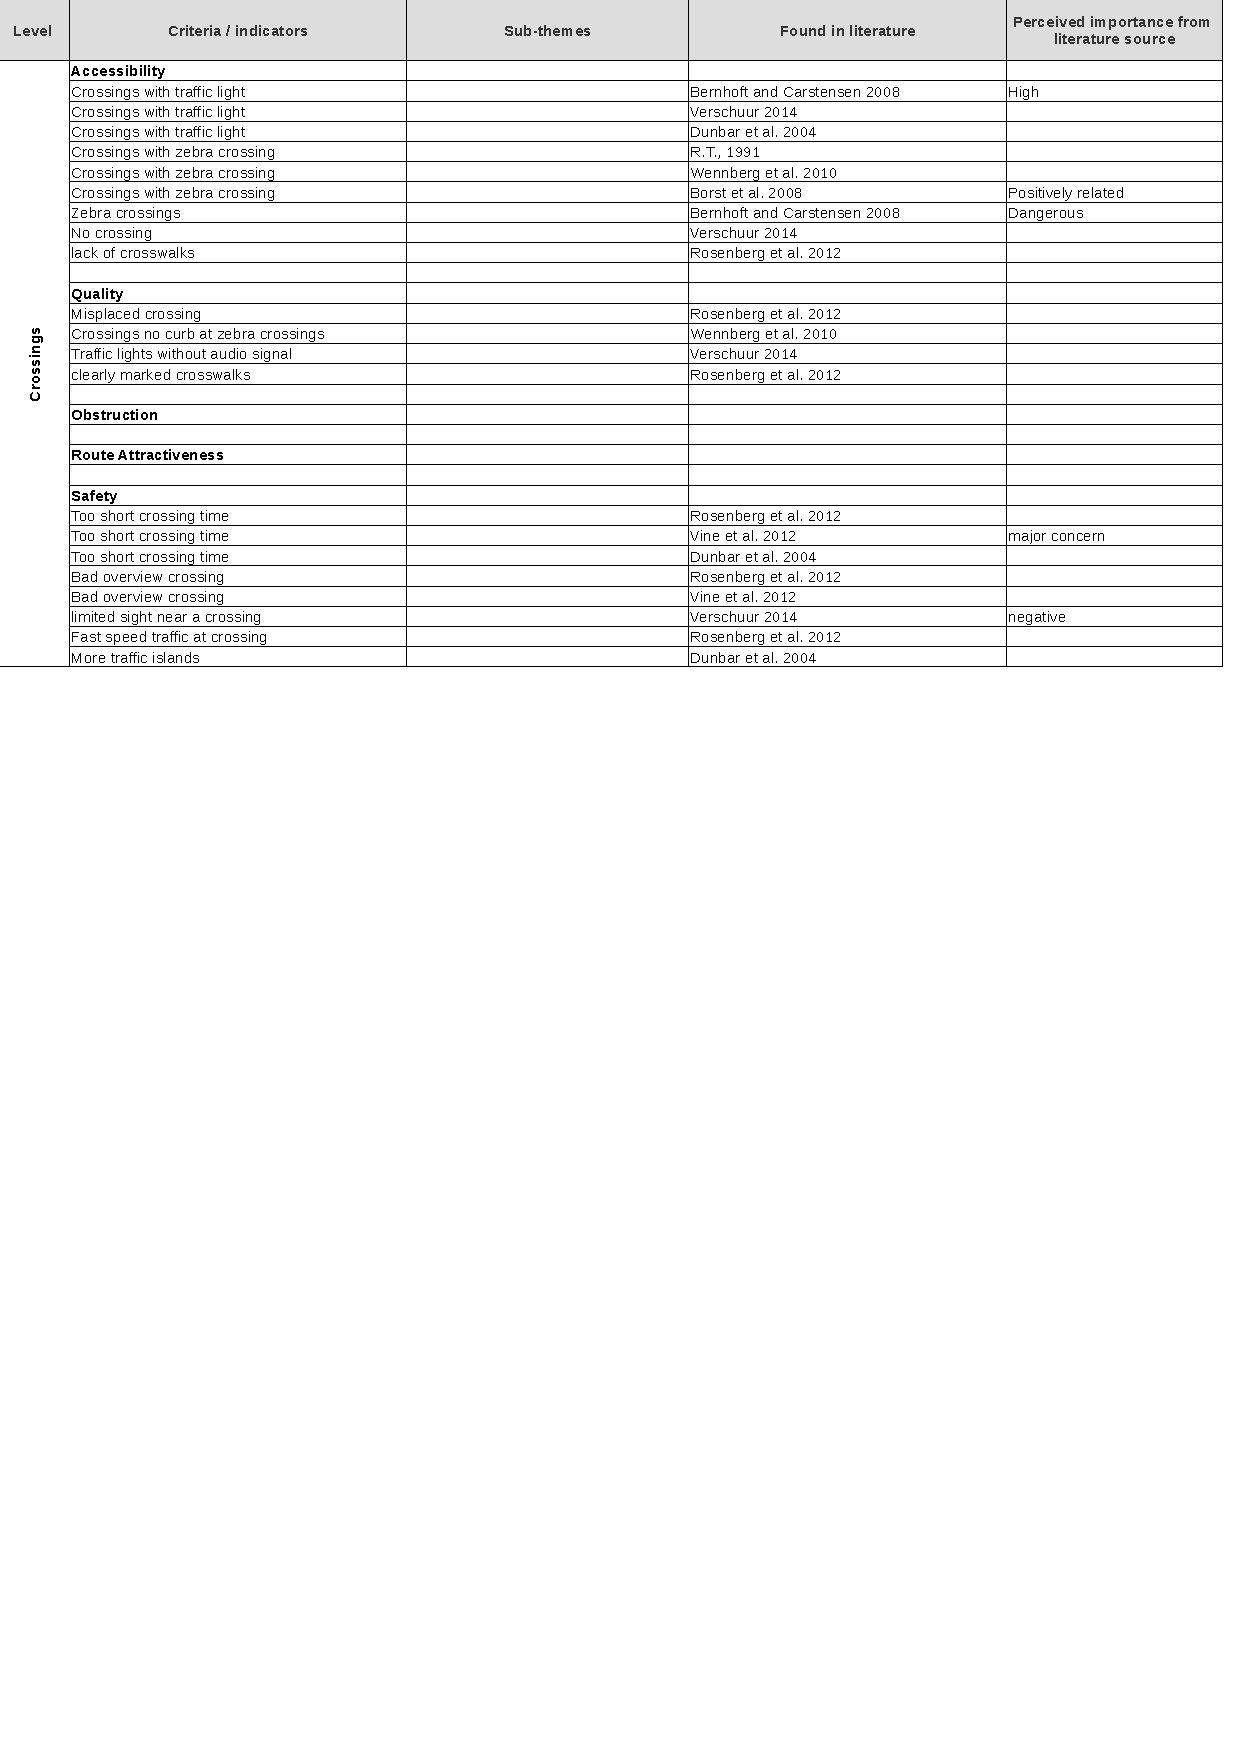
\includepdf[width=\textwidth]{img/annex/A1_crossings_criteria.pdf}
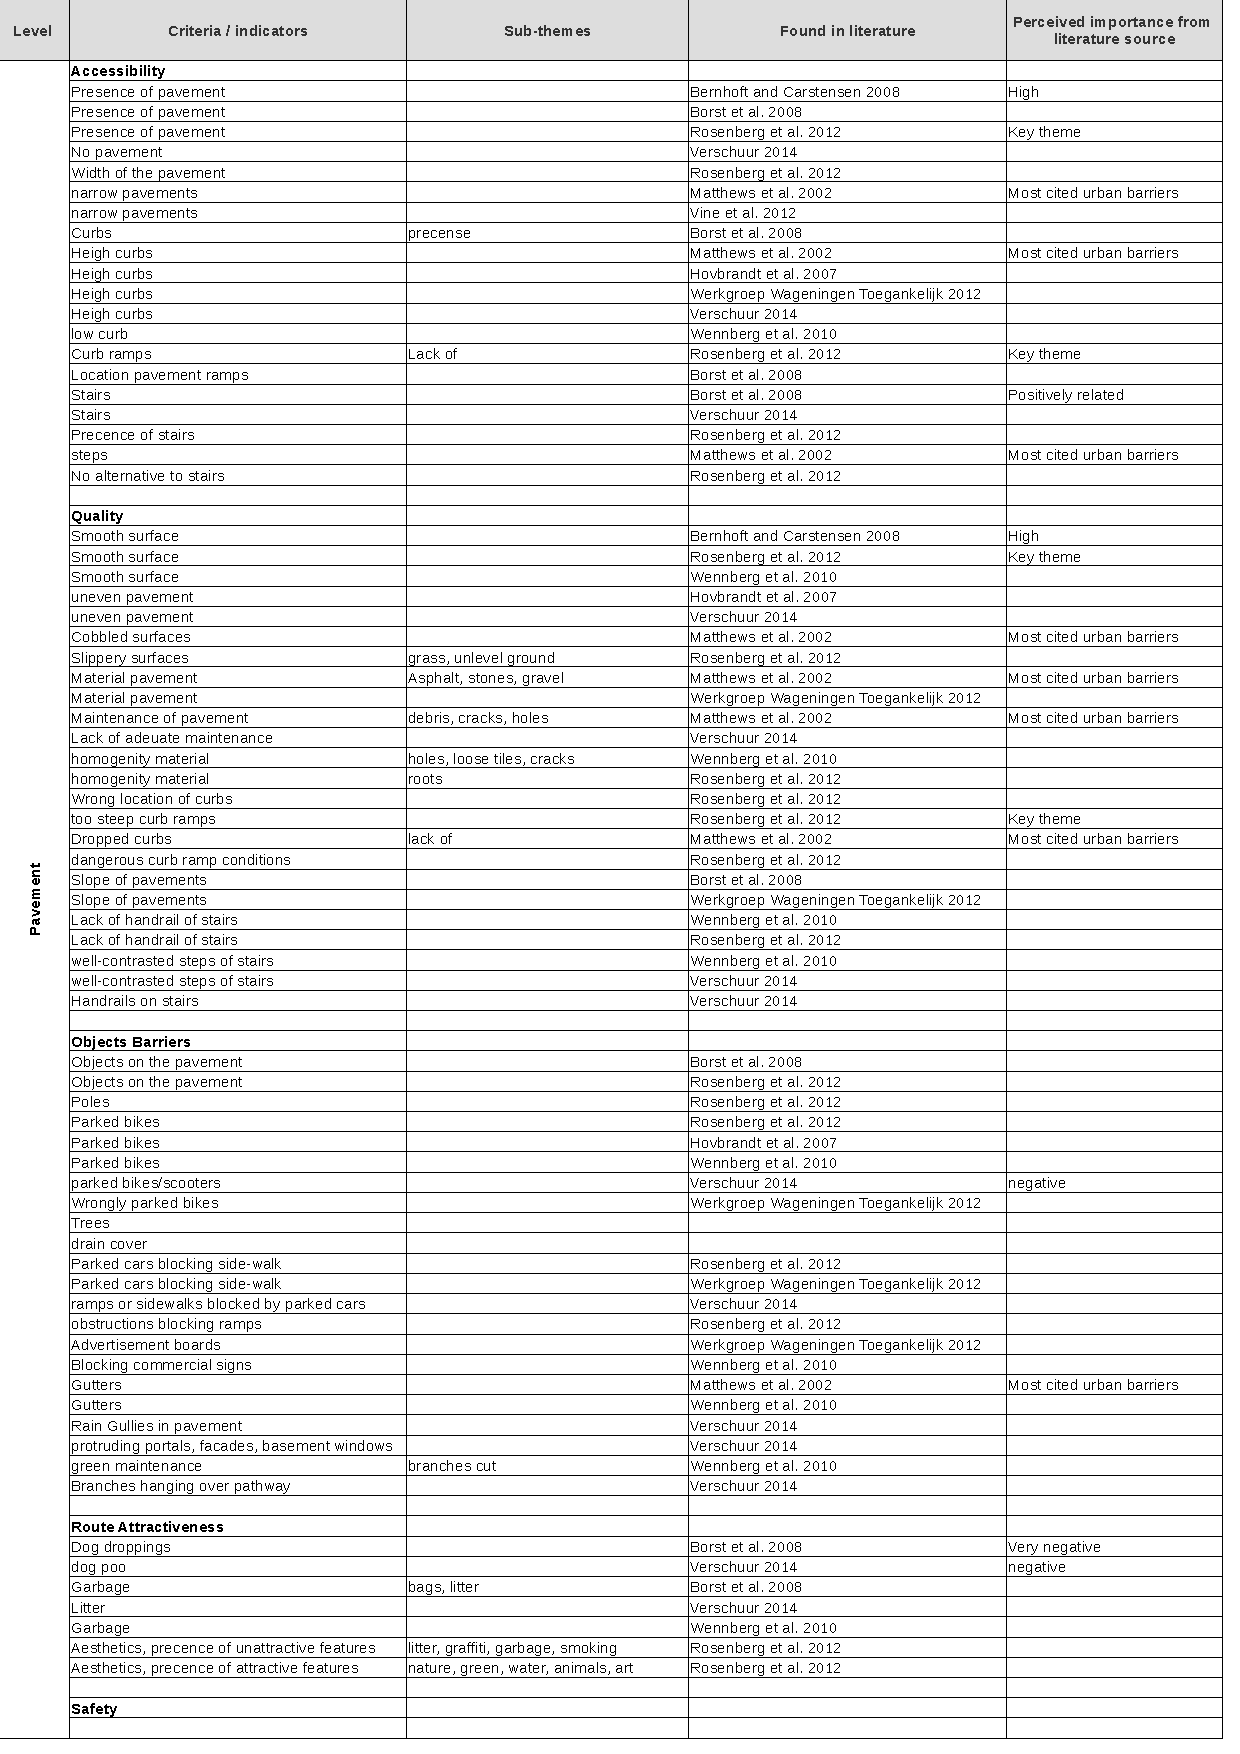
\includepdf[width=\textwidth]{img/annex/A2_pavement_criteria.pdf}
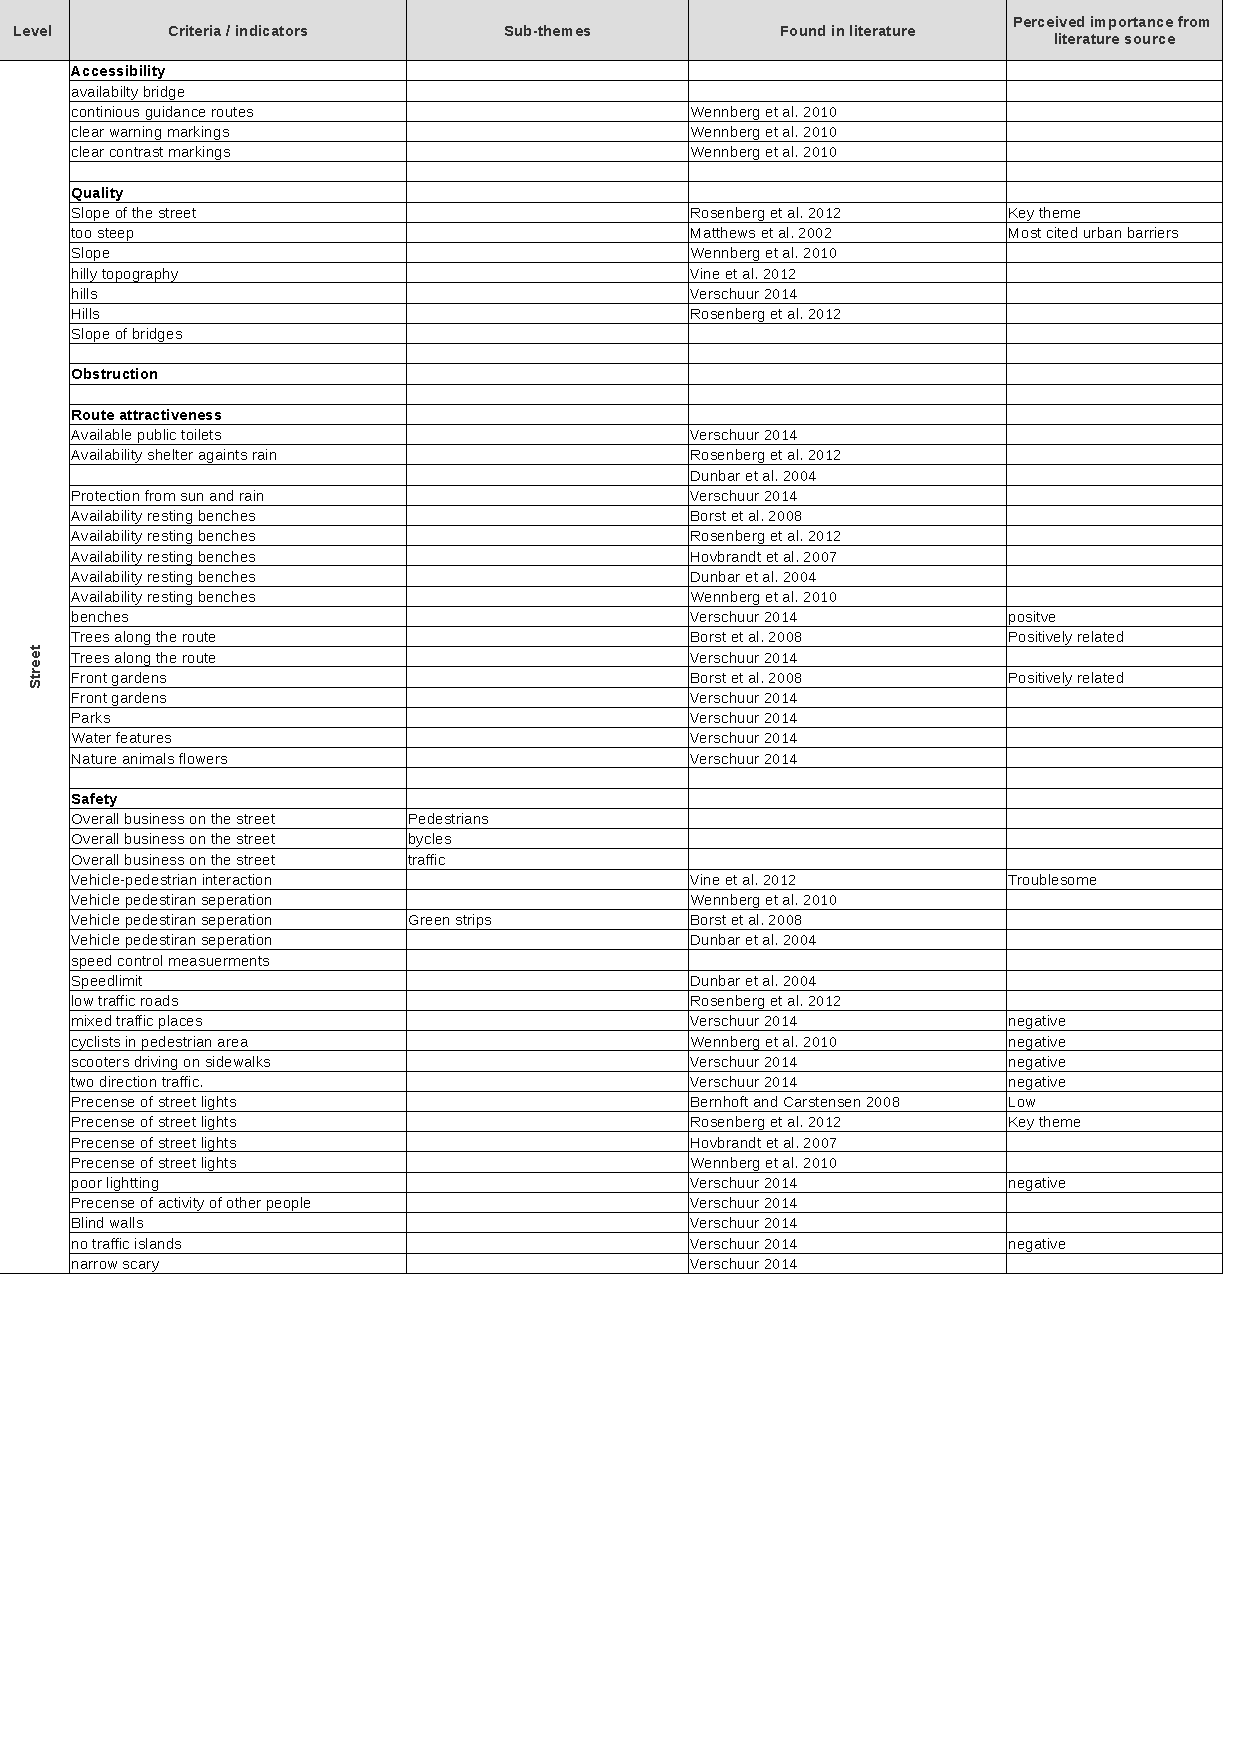
\includepdf[width=\textwidth]{img/annex/A3_street_criteria.pdf}
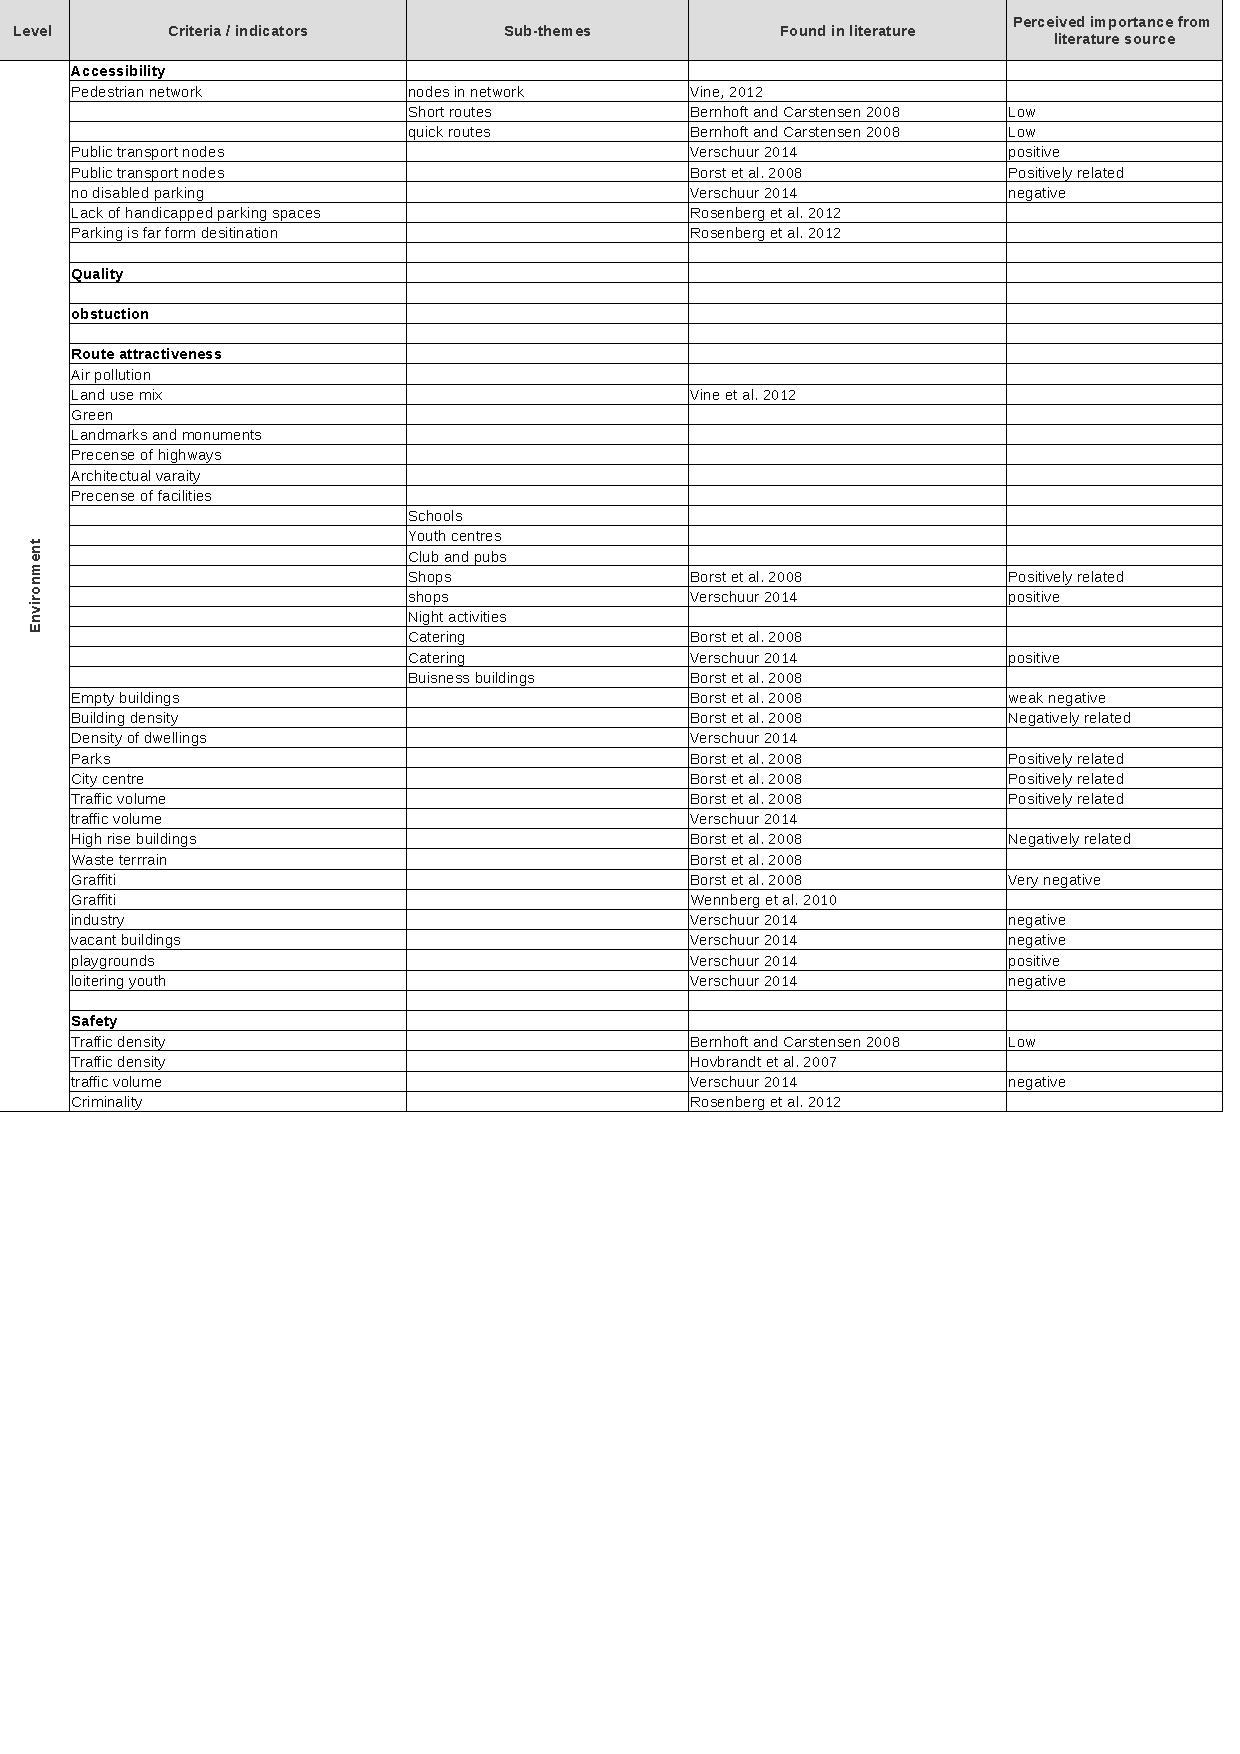
\includepdf[width=\textwidth]{img/annex/A4_environment_criteria.pdf}
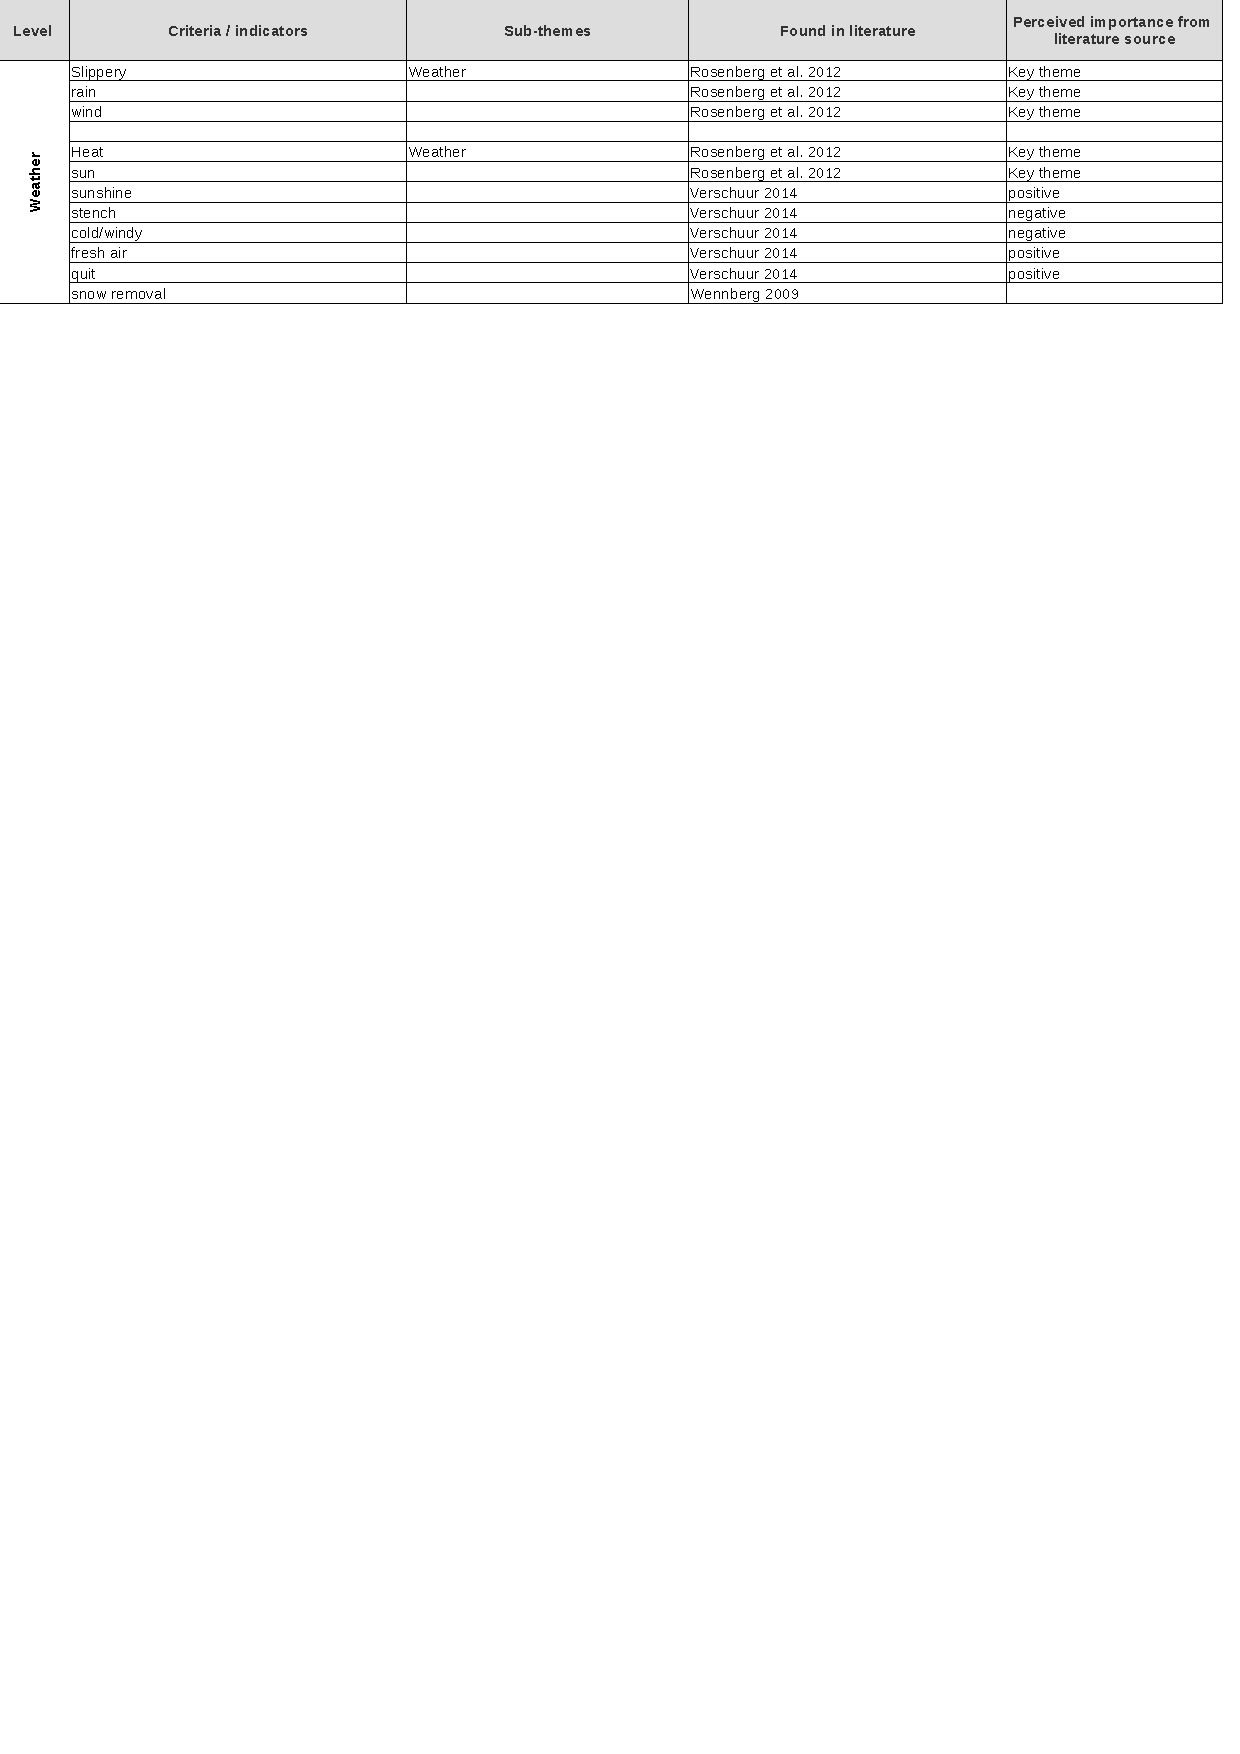
\includepdf[width=\textwidth]{img/annex/A5_weather_criteria.pdf}

\section{Puccini Map Amsterdam}
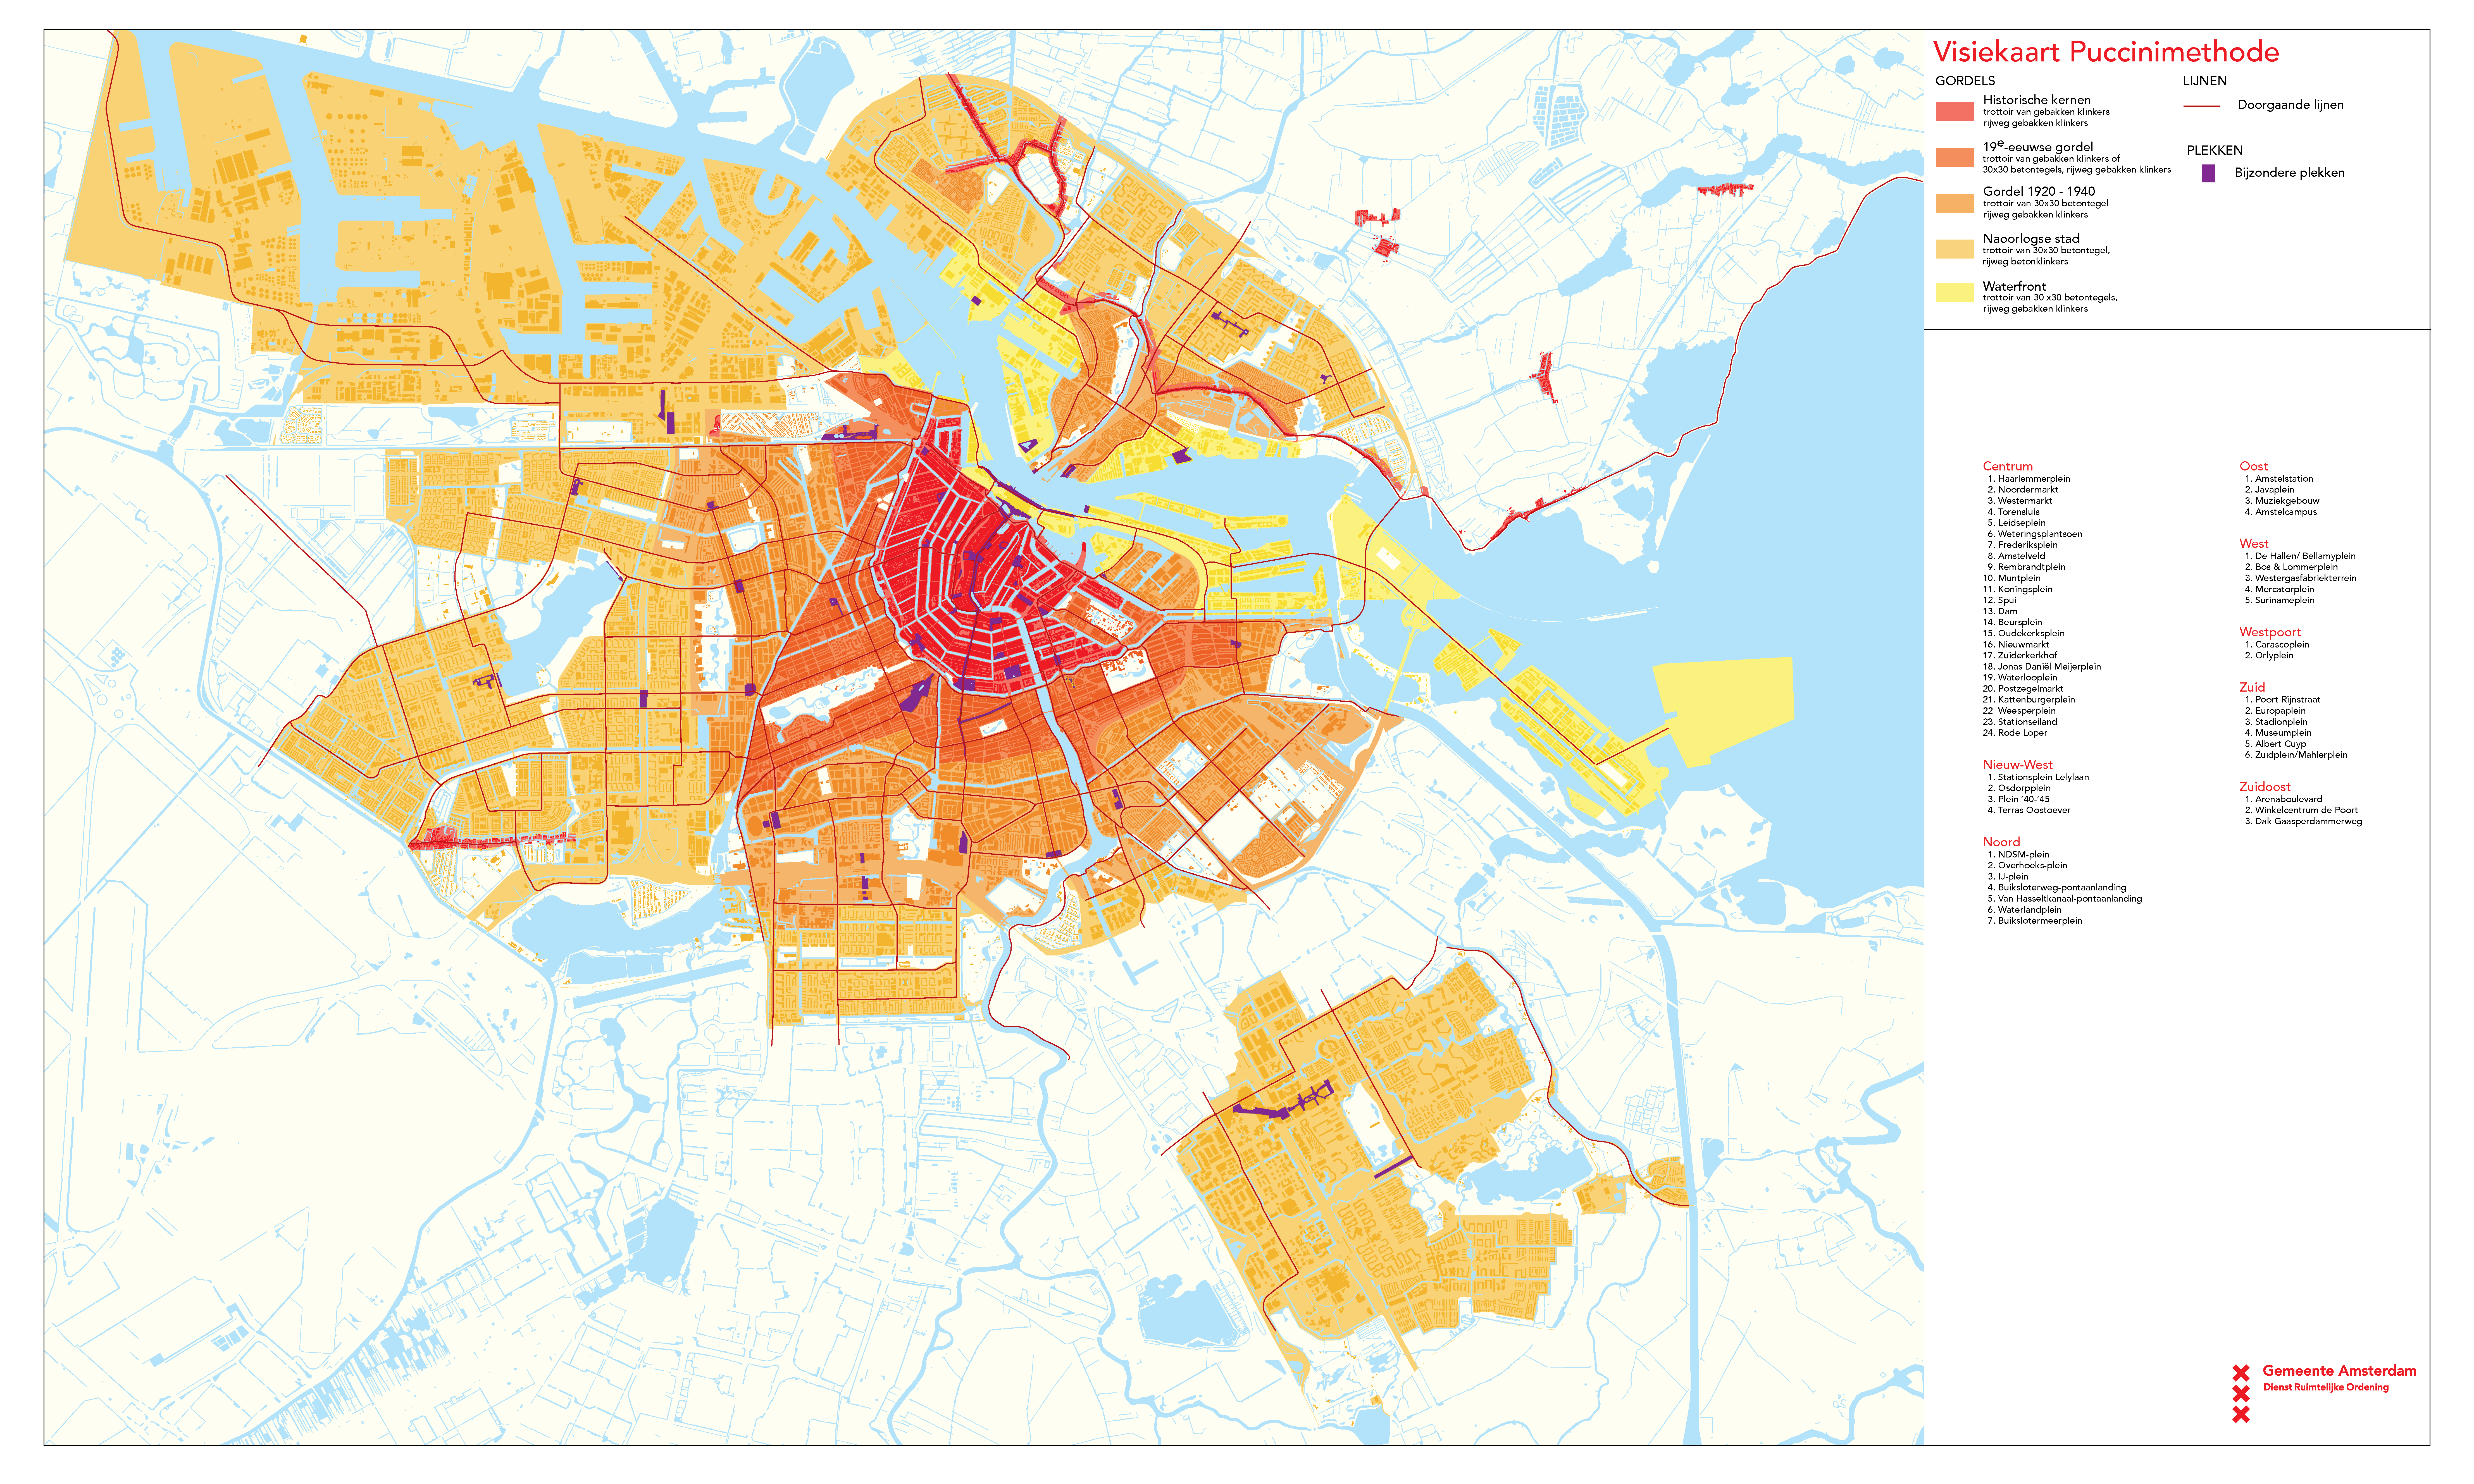
\includepdf[pages=-, scale = 1 , landscape = true ]{img/annex/A_puccini_visiekaart.pdf}\label{pucciniMap}

\clearpage

\section{Questionnaire}\label{Aquest}

\includepdf[pages=-, scale = 1]{img/annex/A_questionaire.pdf}

\clearpage

\section{Accelerometer app alternatives}\label{Aapps}
\textbf{Accelerometer Monitor, Mobile Tools.}
\begin{itemize}
\item Output as .txt file. 
\item Time saved as difference between measurements in milliseconds. No clock-time.
\item $X(m/s^2)$, $Y(m/s^2)$ and $Z(m/s^2)$
\end{itemize}
The Accelerometer Monitor did not give a clock-time bases time stamp, therefore it was hard to link it to the GPS data. Also the .txt output needed some processing before use. 

\textbf{Accelerometer Monitor, keuwlsoft Tools.}
\begin{itemize}
\item Option to safe output on the phone, but only limited amount of readings were done. Then no output was generated any more.
\item Output as .txt file
\item Time as seconds passed. No clock-time
\item $X(m/s^2)$, $Y(m/s^2)$, $Z(m/s^2)$ and $R(m/s^2)$, Theta(deg) and Phi(deg) As given by the application itself. 
\end{itemize}
The Accelerometer Monitor from Keuwlsoft stopped measuring after a random amount of time, so could not be trusted. Also, no clock based time stamp was provided which made it harder to link to the GPS data.

\textbf{AcMeter}
\begin{itemize}
\item No function to save data
\end{itemize}
The AcMeter showed the accelerometer output of the phone on screen, but did not contain a function to save the data. It was not the only application that had only this function, but an example for the many applications that can be found on-line. 

\clearpage

\section{Interviews with elderly list of possible obstacles}\label{Aelderly}
% tabel in annex
% From interviews with elderly list
\begin{enumerate}
	\item = never
	\item = rarely
	\item = sometimes
	\item = often
	\item = always
\end{enumerate}

\begin{table}[ht]
\caption{Average score per possible problem \label{obstacles}}
\begin{tabular}{|l|l|}
	\hline
	 & Average score \\
	\hline
	\multicolumn{2}{|c|}{Quality of the side walk} \\
	\hline
	Bad maintenance of side walks & 4 \\
	Narrow side walks & 1 \\
	too few curb ramps & 3.5 \\
	Sloping side walks & 2.5  \\
	Too steep slopes & 3 \\
	Crossings on bad location & 1 \\
	unclear crossings & 1 \\
	Not enough time for crossing & 2.5 \\
	Mixed use of space & 3 \\
	Bikers on the side walk & 2 \\
	\hline
	\multicolumn{2}{|c|}{Objects} \\
	\hline
	Wrongly parked cars & 4 \\
	Wrongly parked bikes and scooters & 1.5 \\
	Drain covers & 1 \\
	poles on the side walk & 2 \\
	Dog poop & 1 \\
	Not enough resting benches & 1 \\
	Not enough public rest-rooms & 2 \\
	Not enough shelter by rain & 1.5 \\
	protruding portals, facades, basement windows & 3 \\
	\hline
	\multicolumn{2}{|c|}{Overall} \\
	\hline   
	A lot of pedestrians & 3 \\
	A lot of noise & 3 \\
	A lot of traffic & 1.5 \\
	\hline
	\multicolumn{2}{|c|}{Safety} \\
	\hline
	Scary alleys & 1 \\
	Bad lightening by evening/night & 1 \\
	loiterers & 1.5 \\
	Unsafe feeling & 1.5 \\
	\hline
	\multicolumn{2}{|c|}{Environment} \\
	\hline 
	A lack of green & 1 \\
	Bad maintenance & 1 \\
	Ugly buildings & 1.5 \\
	Litter & 1 \\
	Garbage bags & 1.5 \\
	Wind & 1.5 \\
	\hline
\end{tabular}
\end{table}

\clearpage

\section{Failed measurements}\label{Afailed}
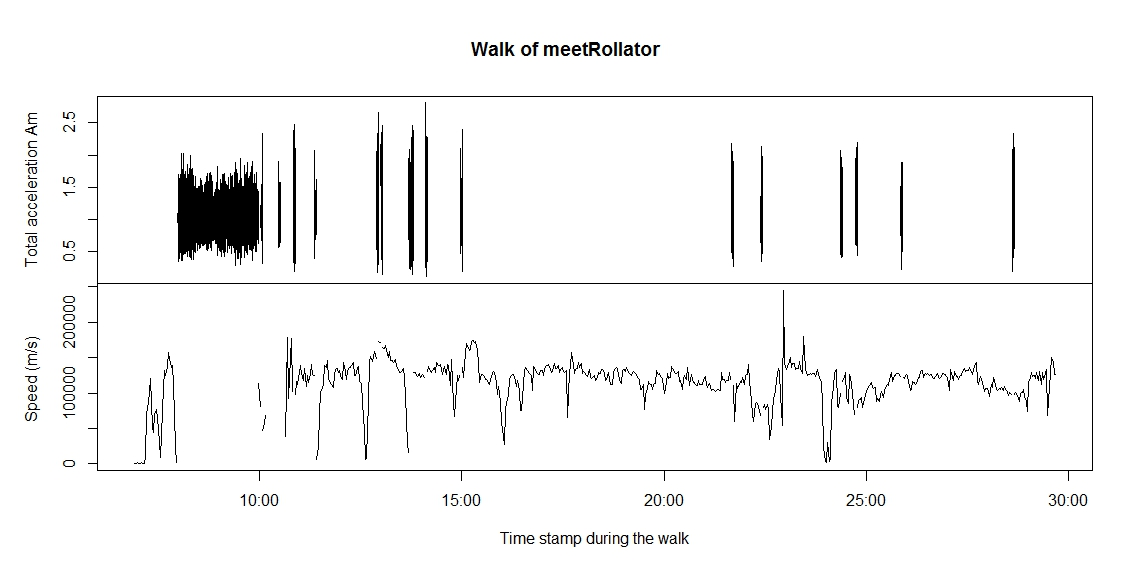
\includegraphics[width=0.85\textwidth]{img/annex/walkmeetrollator.jpeg}
% 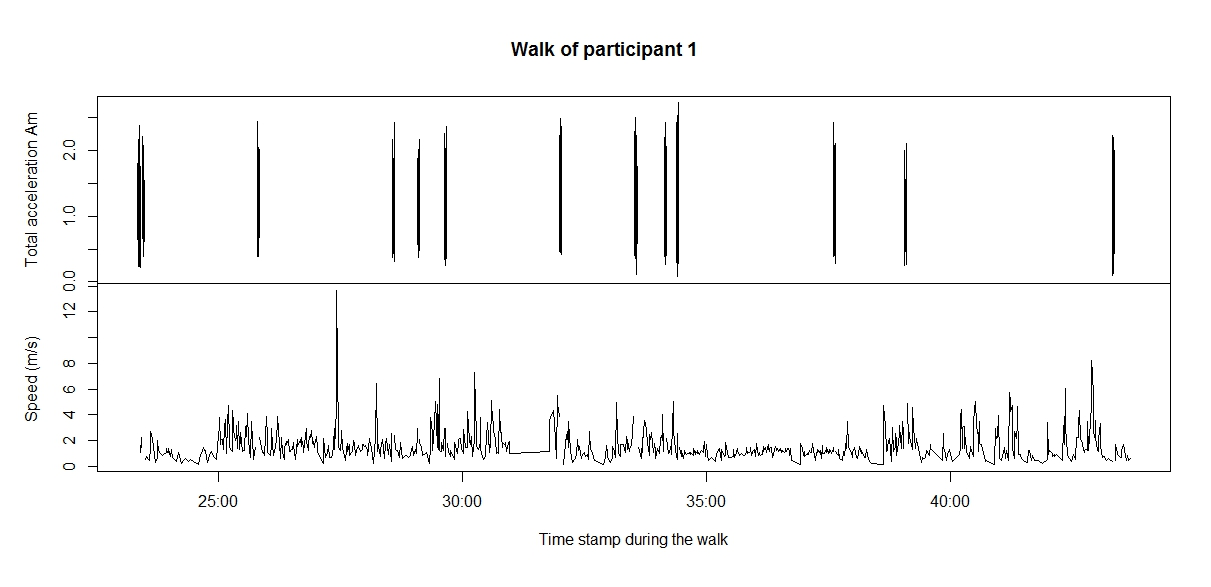
\includegraphics[width=\textwidth]{img/annex/walkpart1}
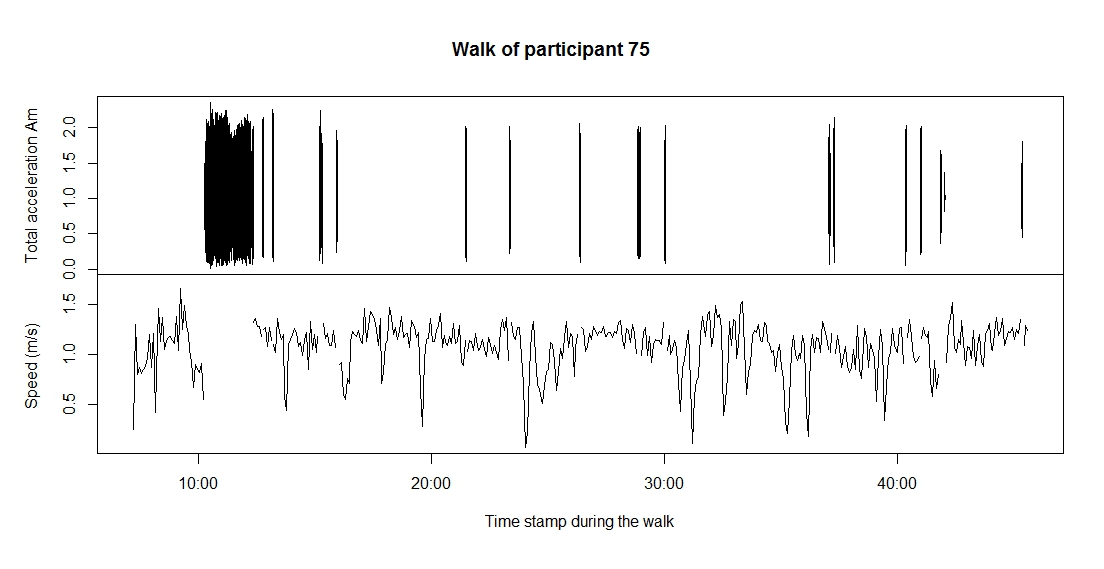
\includegraphics[width=0.85\textwidth]{img/annex/walkpart75.jpeg}
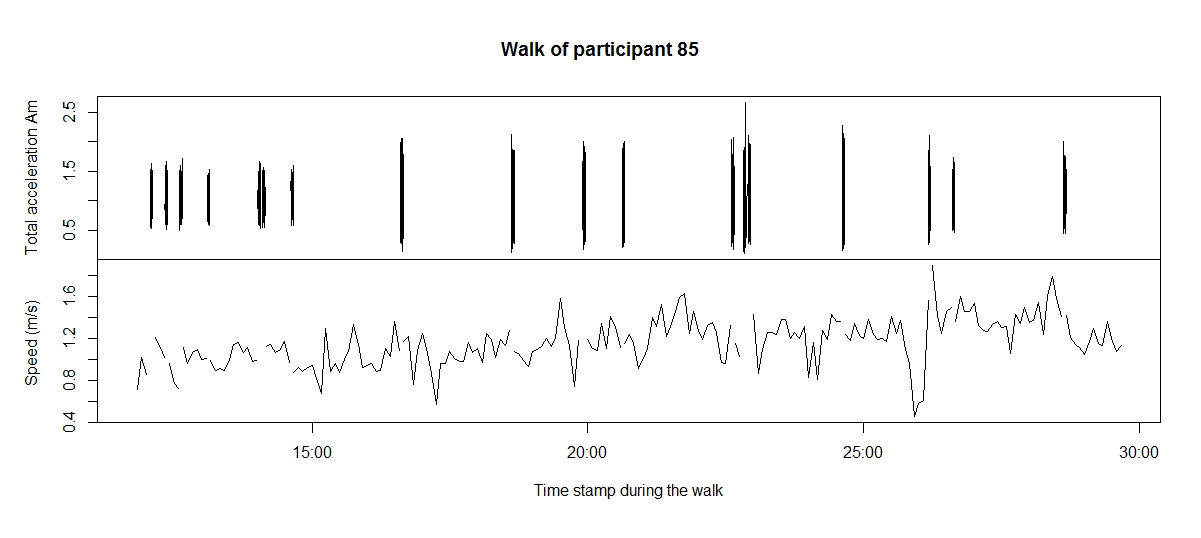
\includegraphics[width=0.85\textwidth]{img/annex/walkpart85.jpeg}
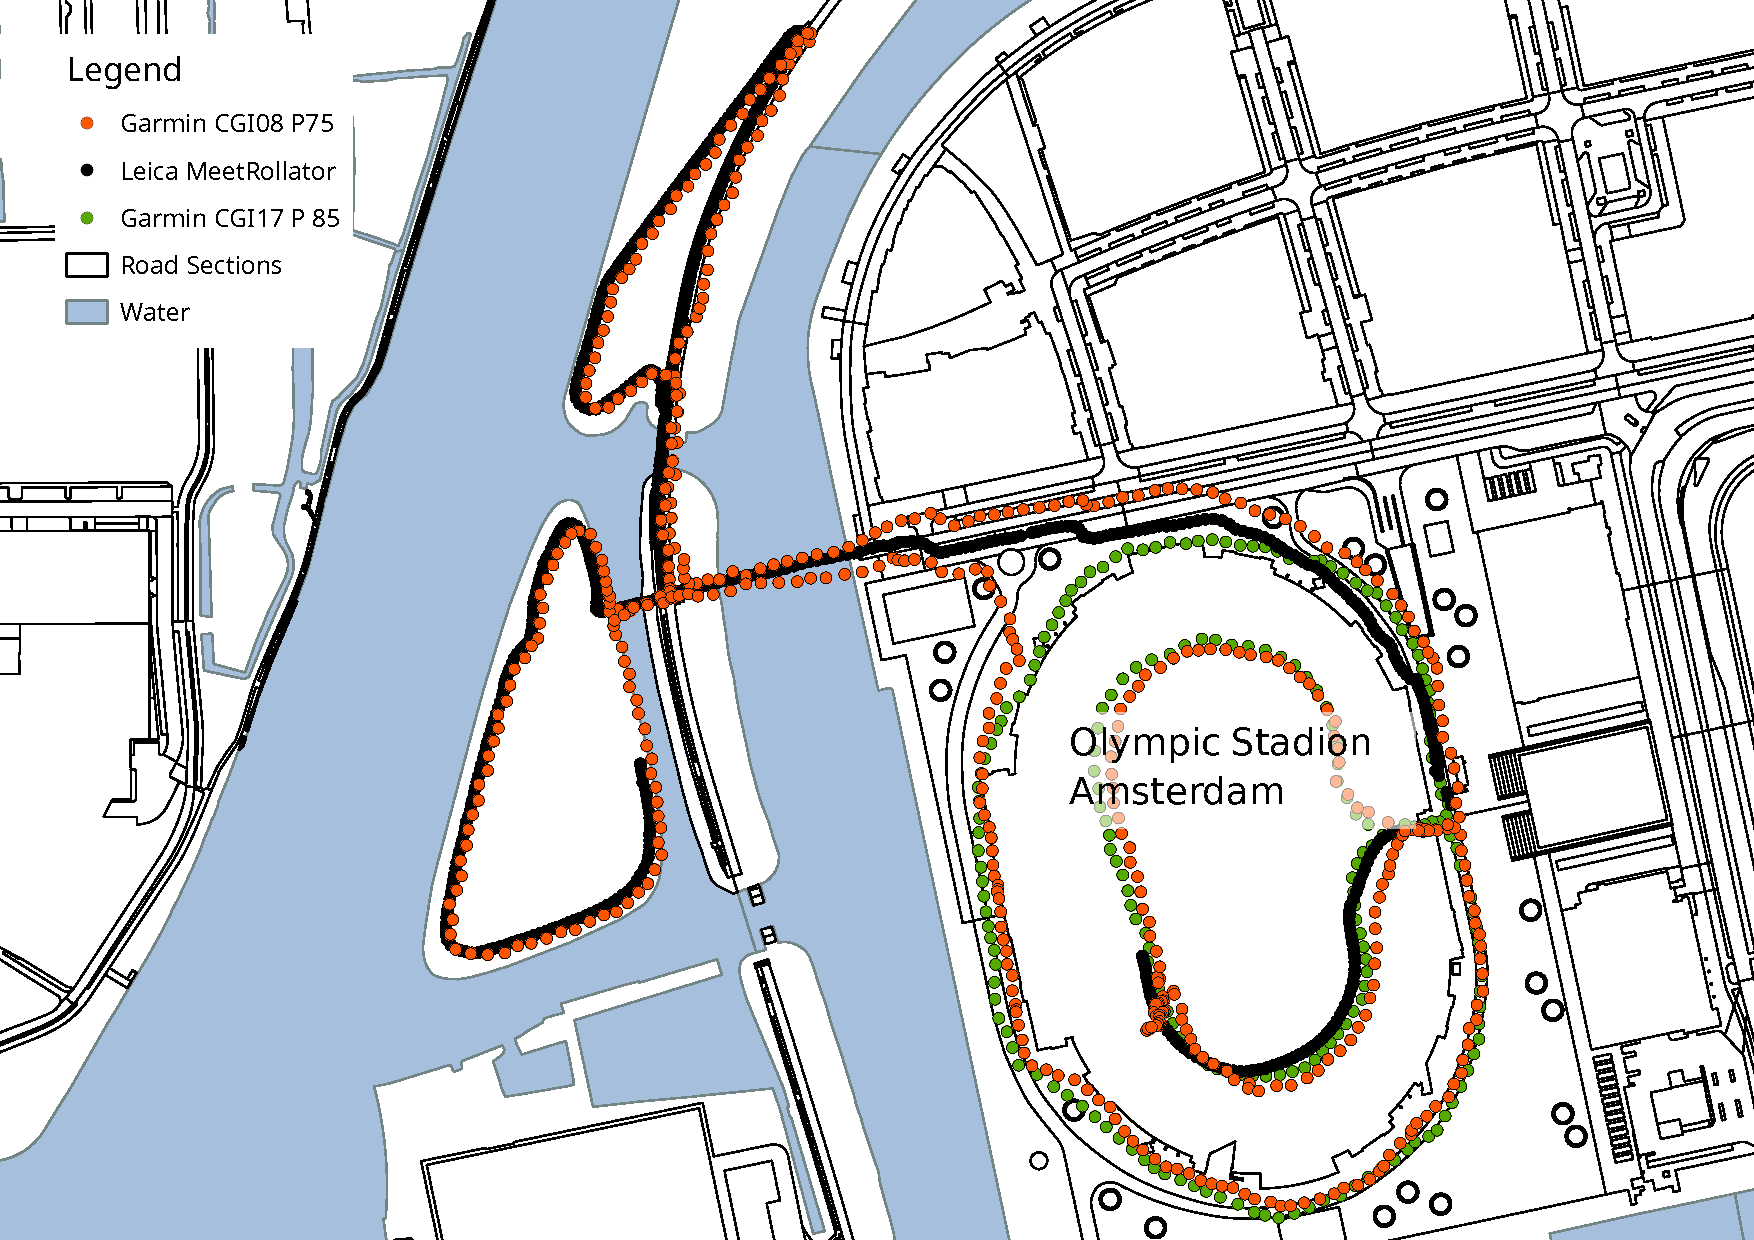
\includegraphics[width=\textwidth]{img/annex/A_failedmeasurementsMap.pdf}

\clearpage

\section{Jordaan road classification total}\ref{Ajordaan}
\includepdf[pages=- , nup=1x1]{img/annex/A_Jordaan_weg_classificatie_resultat.pdf}

\clearpage

\section{Detail of AHN2 of Jordaan}\label{AAHN}
\begin{figure}[h]
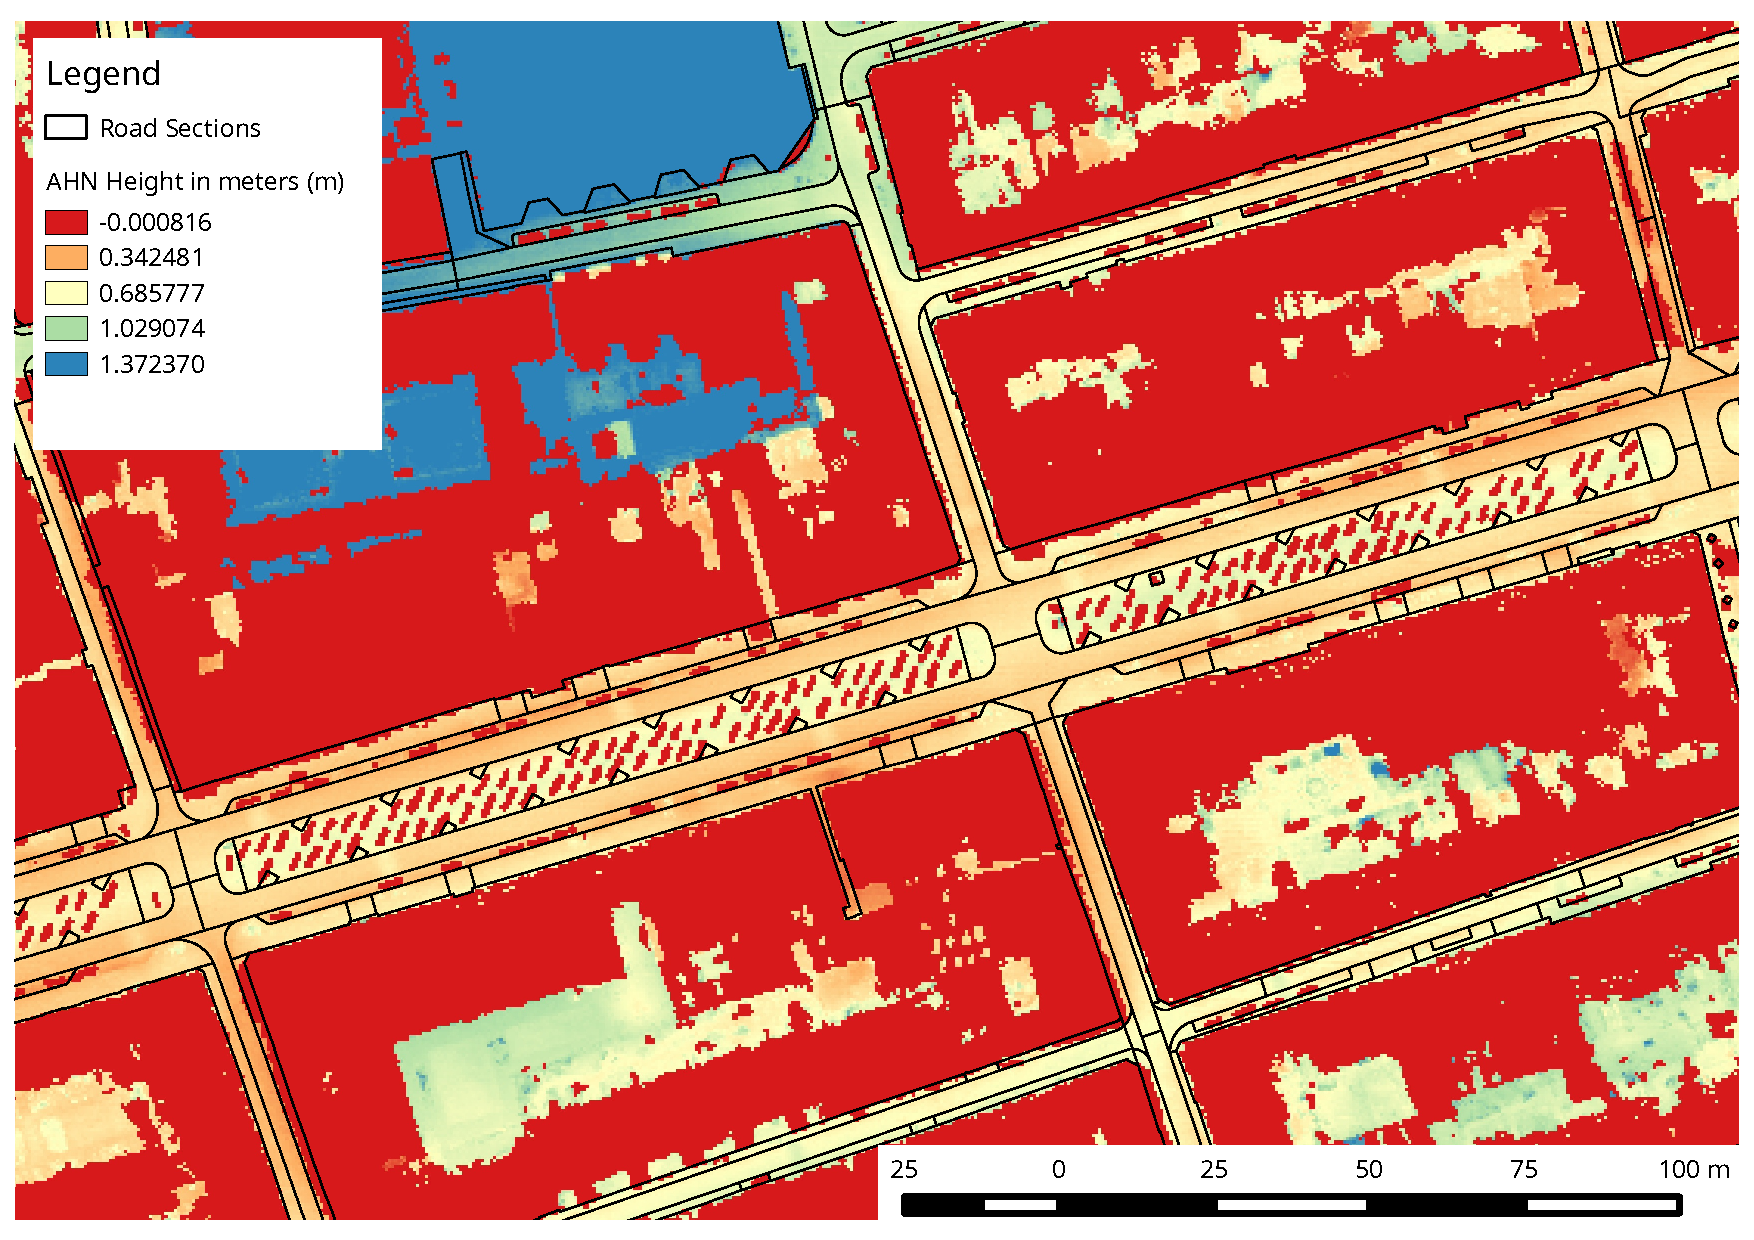
\includegraphics[width=\textwidth]{img/R_AHN_jordaan.pdf}
\centering
\caption{
Detail Jordaan height map\label{jordaanahn}}
\end{figure} 

\clearpage

\section{Change Point methods tests for Speed}\label{Acptest}
\begin{figure}
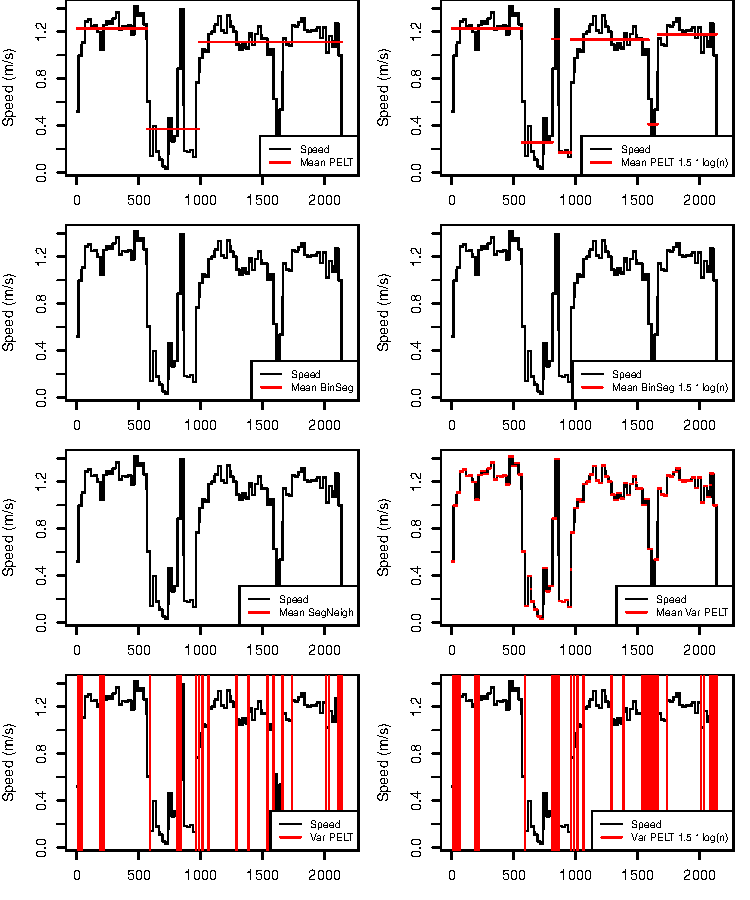
\includegraphics{img/R_comparisonMethodsSpeed2.pdf}
\end{figure}




\end{appendix}


\end{document} %End of thesis.. I wish you were here :'( 
